\documentclass{beamer}

\usetheme{Padova}

\newsavebox{\authbox}
\sbox{\authbox}{ 
	\centering
	\begin{minipage}{0.45\linewidth}
		\centering\normalsize
		\textcolor{white}{Candidato} \par
		\textcolor{white}{Giovanni Bergo}
	\end{minipage}
	\hfill
	\begin{minipage}{0.45\linewidth}
		\centering\normalsize
		\textcolor{white}{Relatore} \par
		\textcolor{white}{Prof. Armir Bujari}
	\end{minipage}
}
\newsavebox{\datebox}
\sbox{\datebox}{
	
	\begin{minipage}{0.45\linewidth}
		\setlength{\parindent}{0.45cm}
		\textcolor{white}{\indent \\
			\hspace*{0.8cm} 25 Settembre 2019}
	\end{minipage}
}
\title{\small{Esame di Laurea in Informatica}}
\subtitle{\textbf{\LARGE{Gestione delle risorse aziendali mediante un sistema ERP in ambito Food and beverage}}}
\author[Giovanni Bergo]{%
	\usebox{\authbox}
}
\institute{\footnotesize{Dipartimento di Matematica ''Tullio Levi Civita''}}
\date{%25 Settembre 2019
\usebox{\datebox}
}


\begin{document}

%\begin{frame}
%\titlepage
%\end{frame}
\maketitle

\begin{frame}{Sommario}
	\tableofcontents
\end{frame}

\section{Introduzione}

\begin{frame}{L'azienda}
	\begin{minipage}[c]{0.45\textwidth}
		
\includegraphics[width=1\linewidth]{figures/logo_synclab}
	\end{minipage}
	\hfill
	\begin{minipage}[c]{0.45\textwidth}
		Settori in cui opera:
		\begin{itemize}
			\item mobile
			\item videosorveglianza
			\item sicurezza delle infrastrutture informatiche aziendali
		\end{itemize}
	\end{minipage}
			
	\vspace{3.0em}
	\large{\uppercase{Software Gestionale}}
	\begin{itemize}
		\item integra tutti i processi di business rilevanti di un'azienda
	
	\end{itemize}
\end{frame}

\section{Progetto}
\begin{frame}{Proposta di stage}
	\begin{alertblock}{Scopo}
		Lo scopo dello stage \`e  quello di realizzare dei moduli Odoo che fanno riferimento a problematiche in ambito \textbf{Food and beverage} che si occupano di monitorare il ciclo di vita degli alimenti e delle bevande.
	\end{alertblock}
	Principali caratteristiche utilizzate:
	\begin{itemize}
		\item Fatturazione degli alimenti;
		\item Gestione inventario;
		\item Gestione risorse umane;
		\item Gestione vendite e acquisti.
	\end{itemize}
\end{frame}

%\begin{frame}{Tool aziendale}
%L'azienda utilizza Odoo perchè offre una suite di prodotti software molto vasta e per la sua semplicità di utilizzo
%\begin{figure}[H]
%	\begin{center} 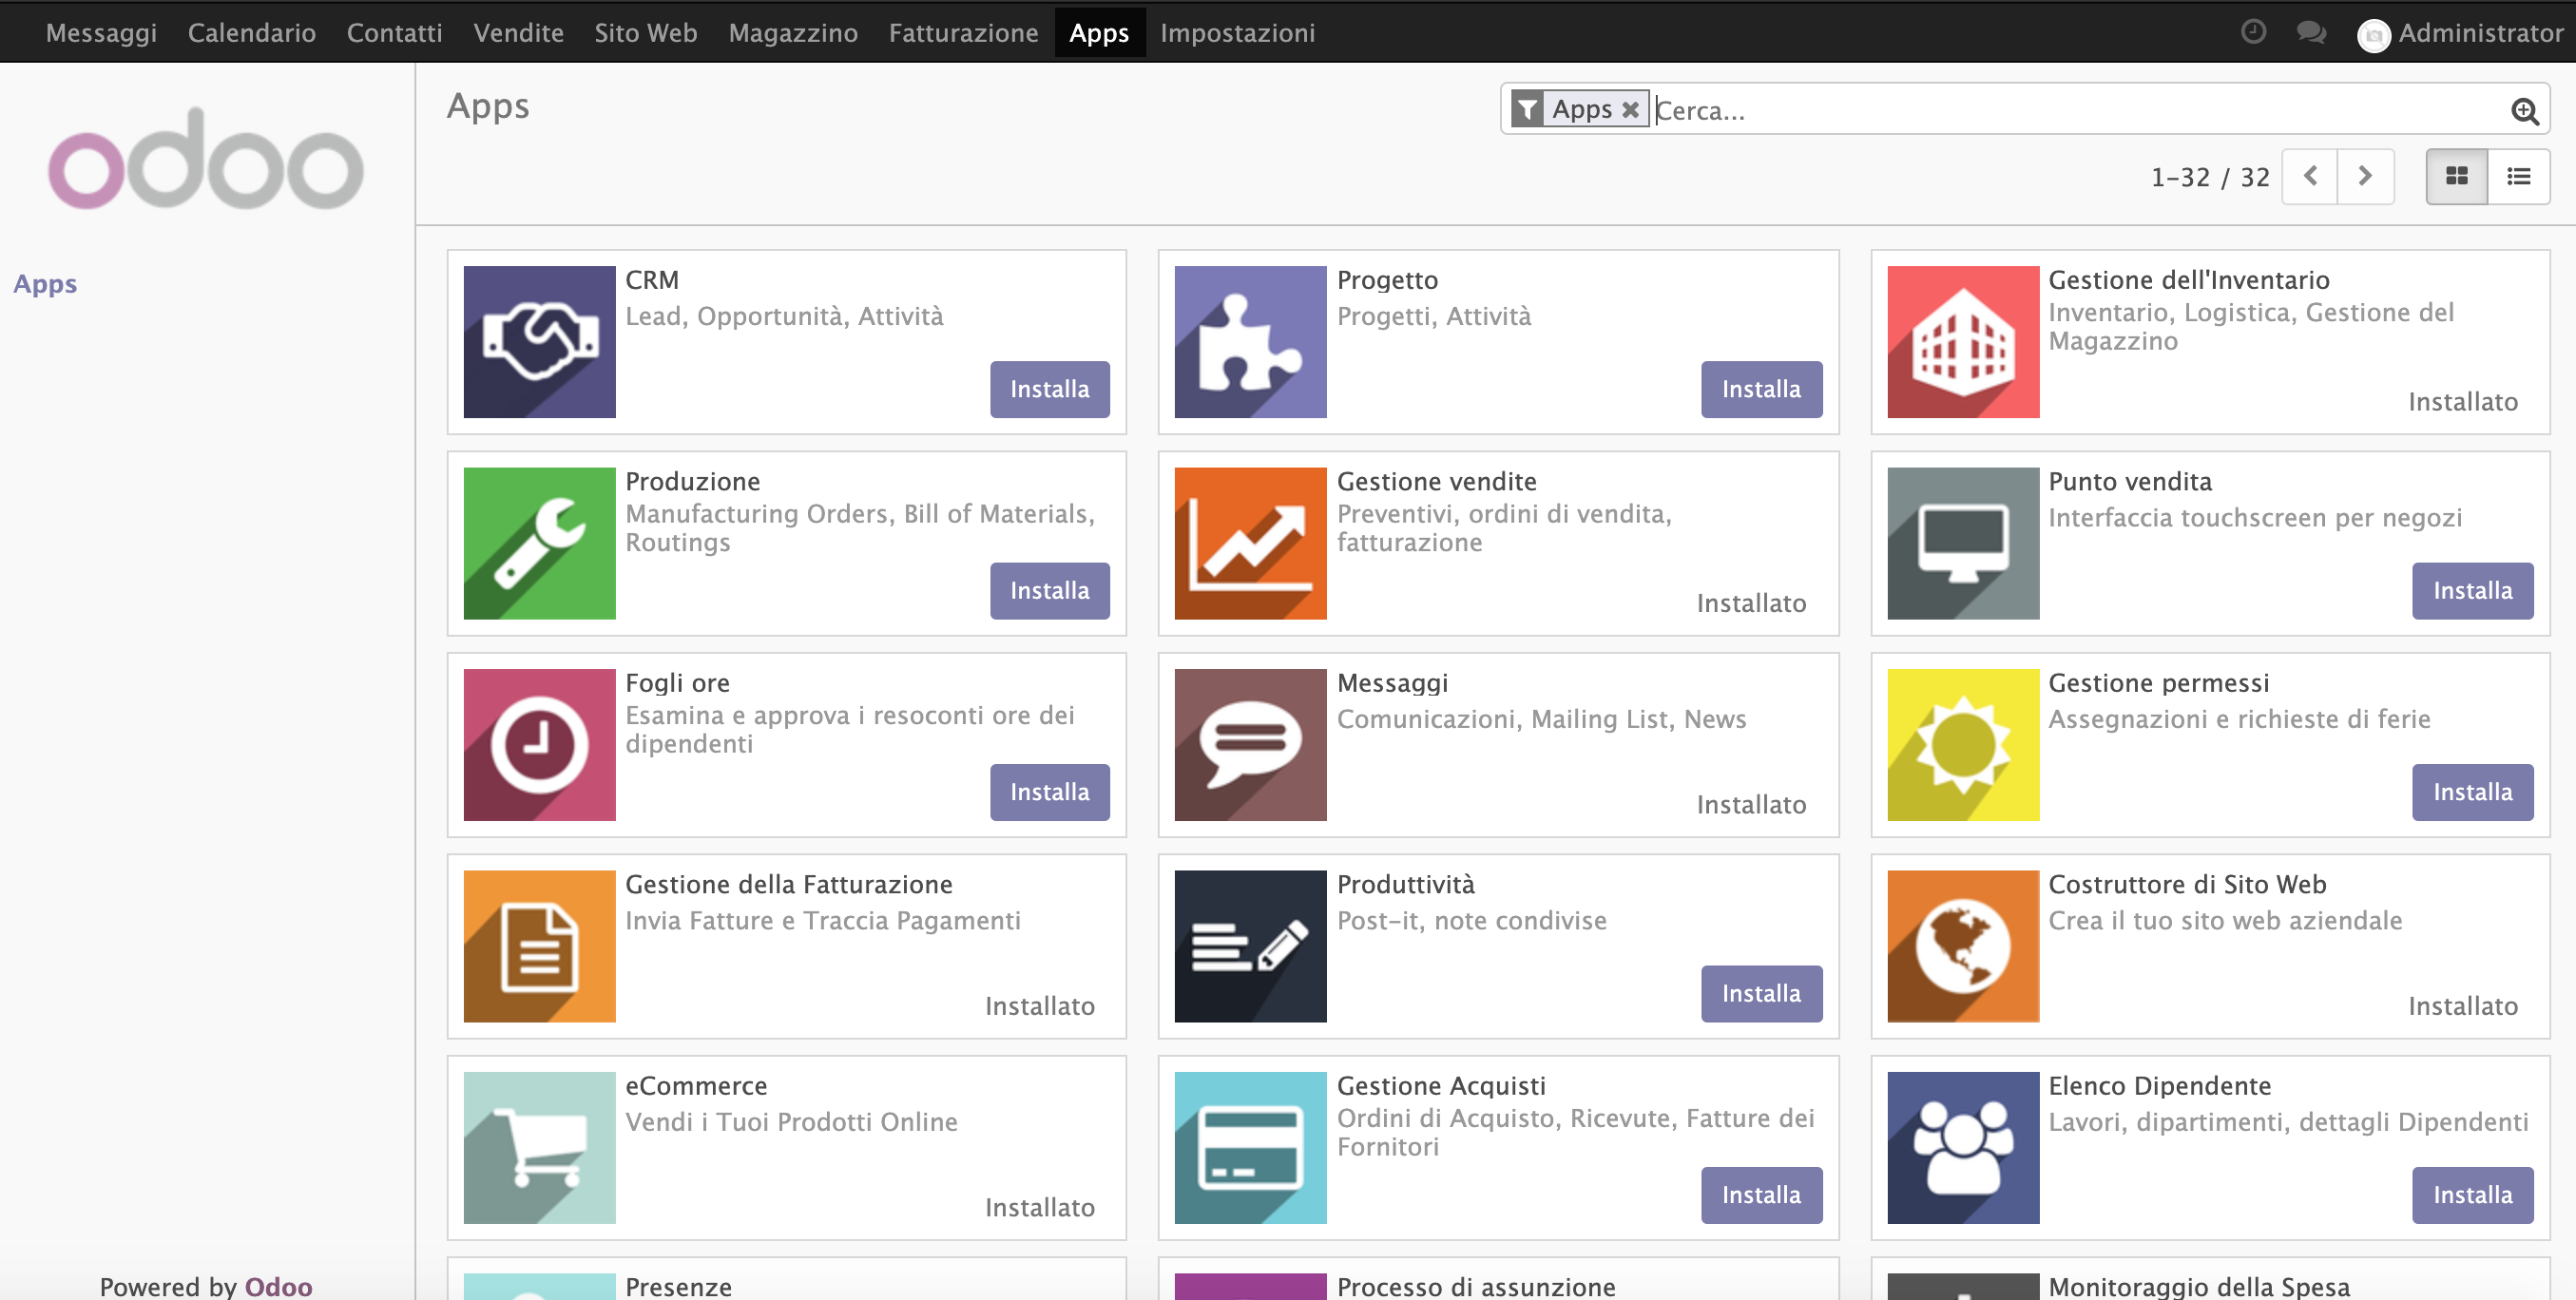
\includegraphics[width=1\linewidth]{figures/odoo}
%	\end{center}
%\end{figure}
%\end{frame}

\section{Tecnologie}
\begin{frame}{Tecnologie}
\vspace*{0.5cm}
\begin{minipage}[c]{0.3\textwidth}
	\begin{figure}
		\centering
		\vspace*{0.5cm}
		
\includegraphics[width=1cm]{figures/orm}
		\caption{API ORM}
		
		
\includegraphics[width=1cm]{figures/python}
		\caption{Python}
		
\includegraphics[width=1cm]{figures/logo_odoo}
		\caption{Odoo}
		
\includegraphics[width=1cm]{figures/Logo_PyCharm}
		\caption{PyCharm}
	\end{figure}
\end{minipage}
\hfill
\begin{minipage}[c]{0.6\textwidth}
	\begin{figure}
		\centering
		
\includegraphics[width=1cm]{figures/openproject}
		\caption{OpenProject}

		
\includegraphics[width=1cm]{figures/Logo_Postgresql}
		\caption{pgAdmin}

		
\includegraphics[width=1cm]{figures/homebrew}
		\caption{Homebrew}

	\end{figure}
\end{minipage}		
\end{frame}

\section{Moduli Odoo}
\begin{frame}{Modulo standard}
\begin{minipage}[c]{1\textwidth}
Un modulo Odoo contiene i seguenti elementi:

\begin{itemize}
	\item \textbf{Classi Python} Manipolano file XML.
	\item \textbf{File di dati} File XML che dichiarano metadati (viste);
	\item \textbf{Controller Web} Gestire le richieste dai browser Web;
	\item \textbf{Dati web statici} Immagini, file CSS o javascript utilizzati dall'interfaccia Web.
\end{itemize}
\end{minipage}

\hfill
\begin{minipage}[c]{0.45\textwidth}
	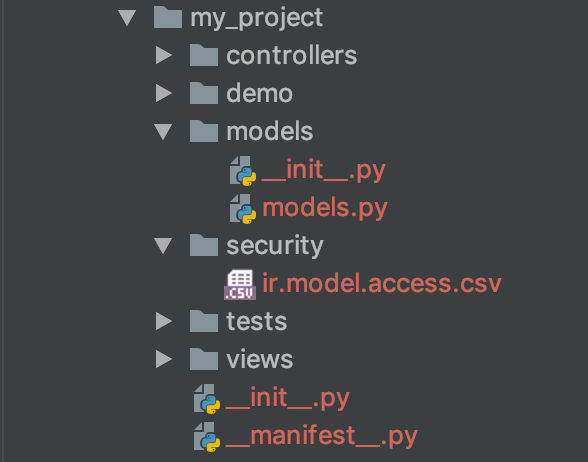
\includegraphics[width=0.7\linewidth]{figures/structure_odoo}
\end{minipage}

\end{frame}

\begin{frame}{Moduli sviluppati}

	\begin{figure}[H]
	\begin{center} 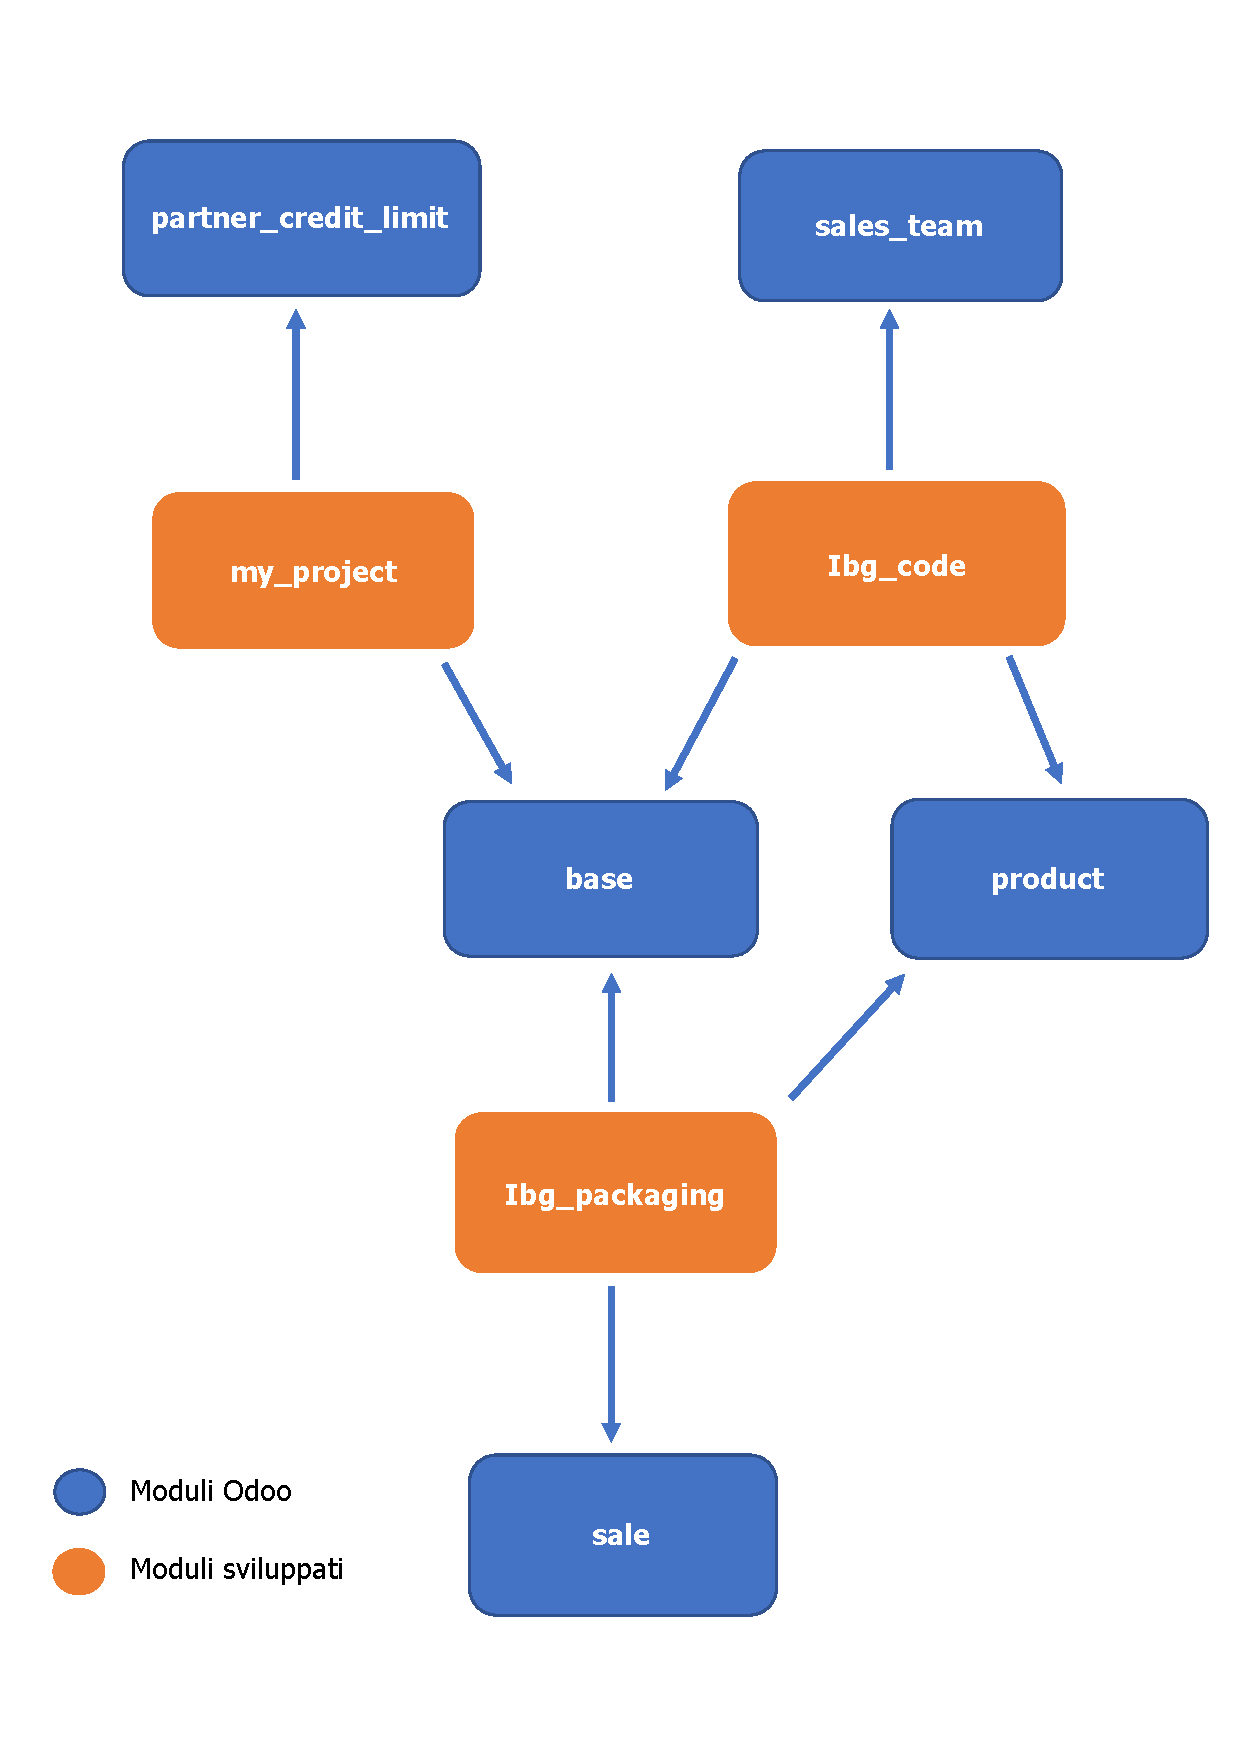
\includegraphics[width=0.51\linewidth]{figures/diagramma}
	\end{center}
\end{figure}


\end{frame}

\begin{frame}{Limite di credito del partner\scriptsize{(my\_project)}}
	\vspace{.5em}
	\begin{alertblock}{Obiettivo}
	Si esegue il confronto tra l'importo dell'ordine di vendita da approvare e il limite di credito del partner. Se il limite di credito del partner è inferiore all'importo di vendita, non consente di approvare l'ordine di vendita.
	\end{alertblock}	


\end{frame}


%\begin{frame}{Limite di credito}
%	\begin{figure}[H]
%	\begin{center} 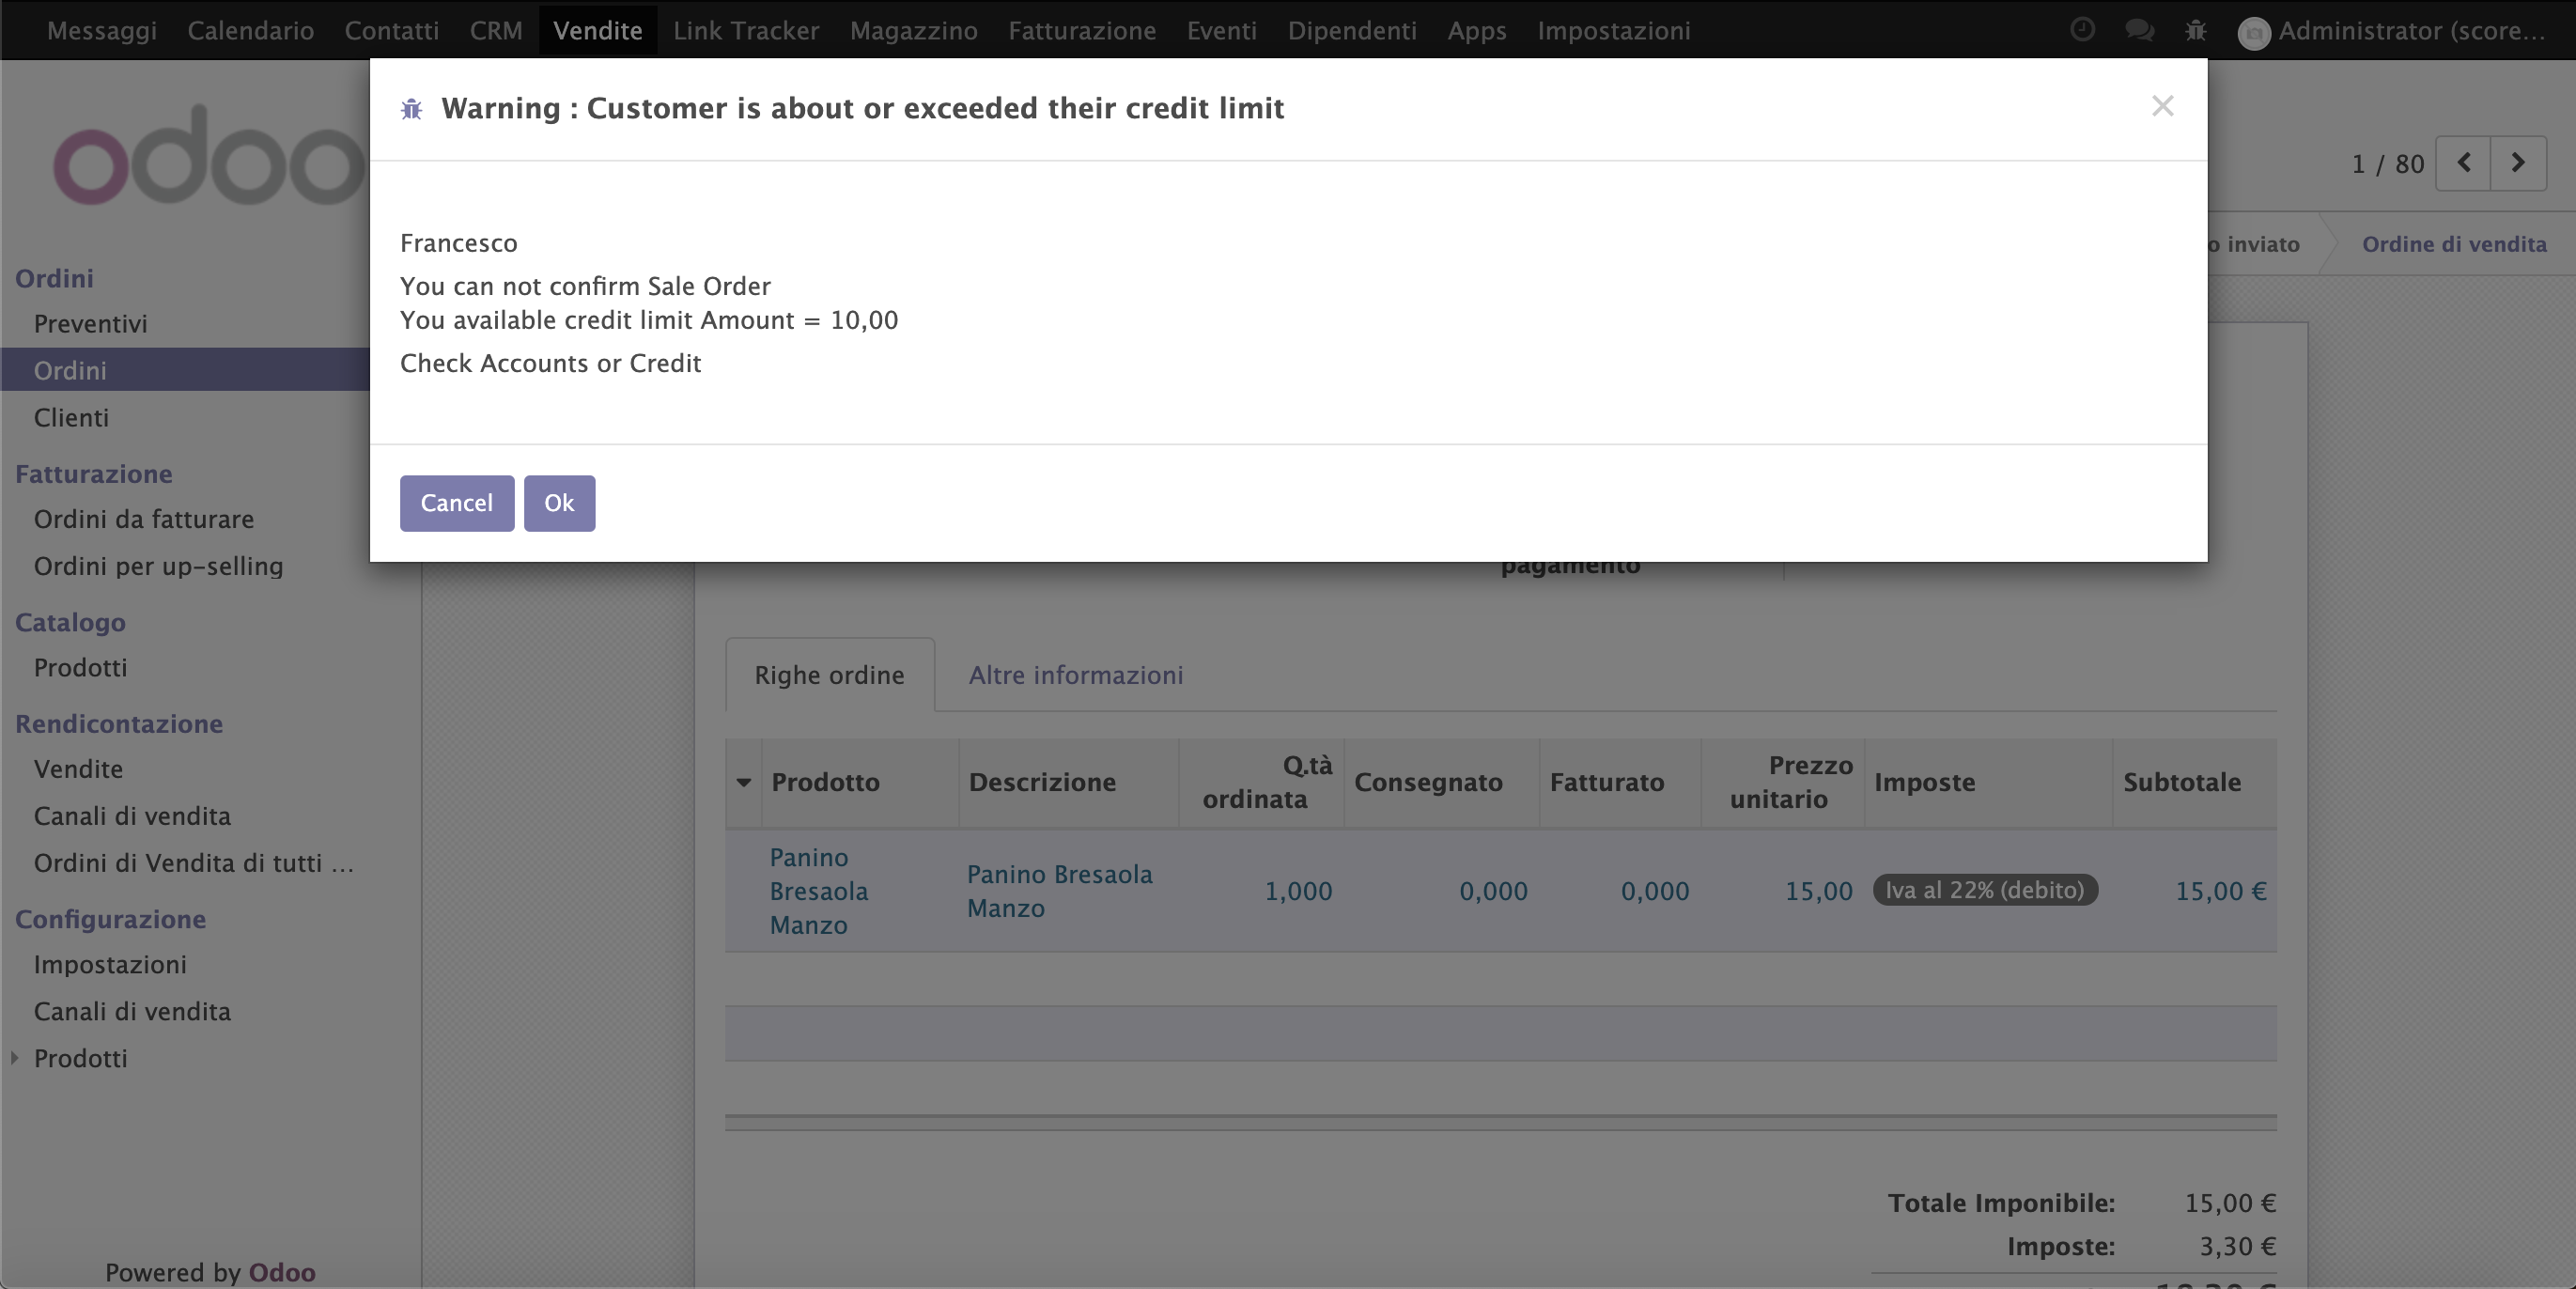
\includegraphics[width=1\linewidth]{figures/check_limit}
%	\end{center}
%\end{figure}
%
%\end{frame}




%\begin{frame}{Blocco Scaduto}
%\begin{figure}[H]
%	\begin{center} 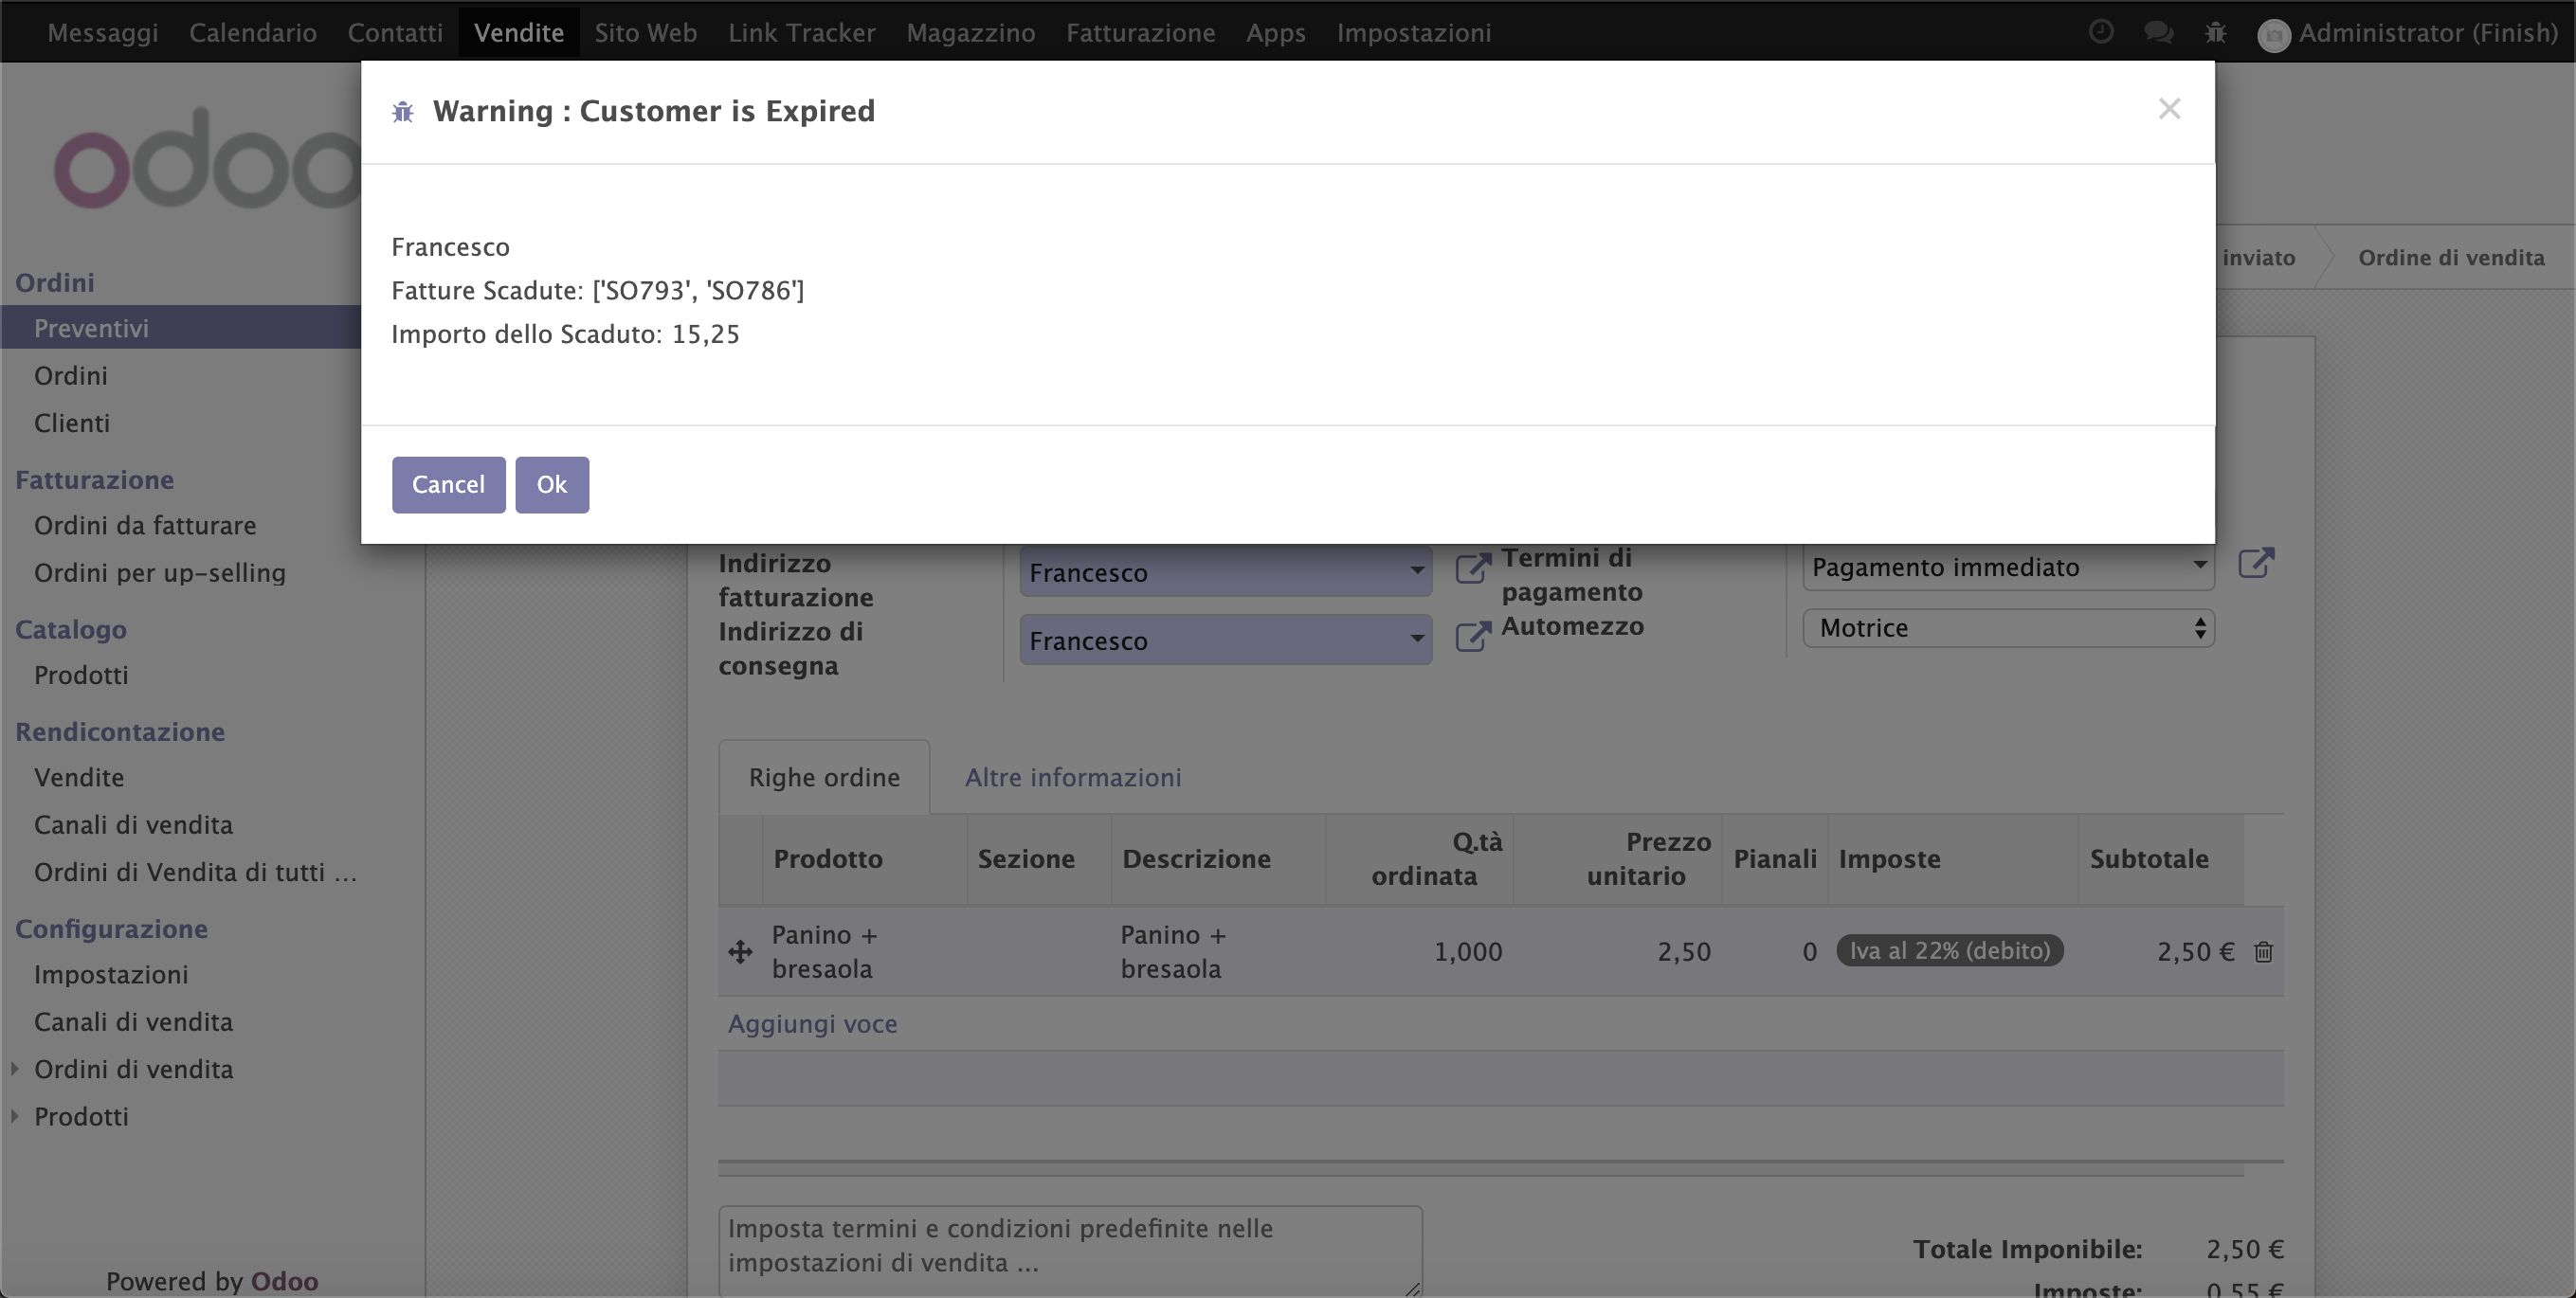
\includegraphics[width=1\linewidth]{figures/check_expired}
%	\end{center}
%\end{figure}
%
%\end{frame}


% CANALI di Vendita

%\begin{frame}{Canali di Vendita\scriptsize{(ibg\_code)}}
%
%\begin{figure}[H]
%	\begin{center} 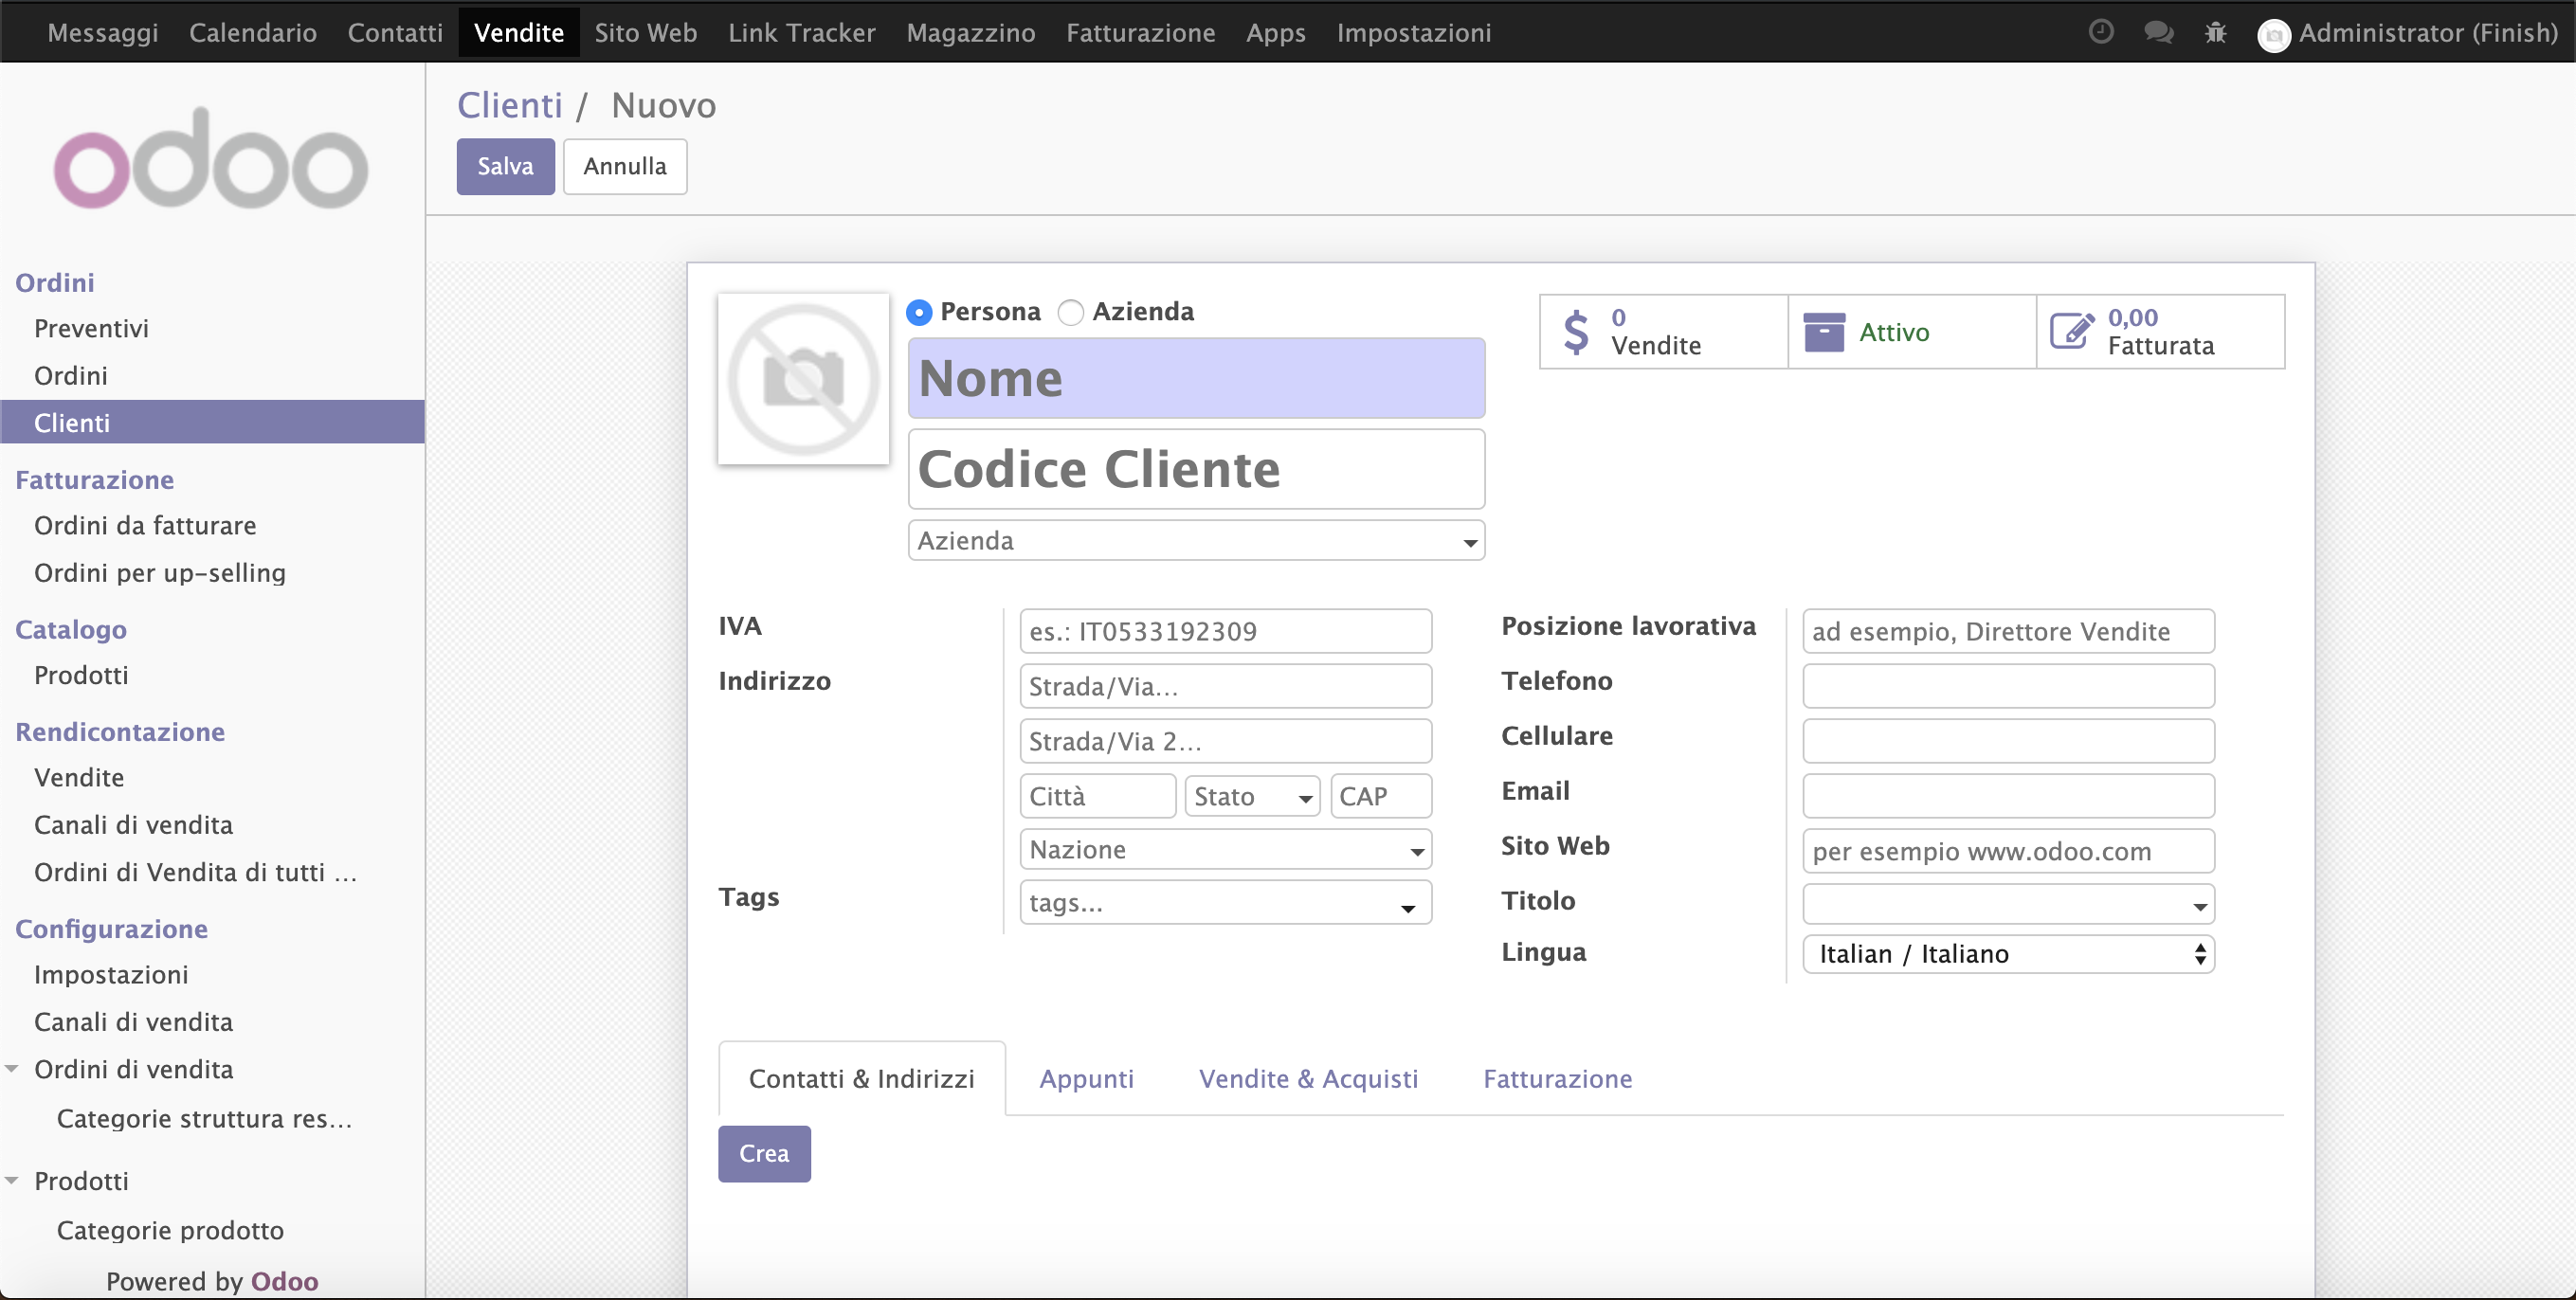
\includegraphics[width=1\linewidth]{figures/ibg_code}
%	\end{center}
%\end{figure}
%
%\end{frame}

%\begin{frame}{Canali di Vendita}
%
%\begin{figure}[H]
%	\begin{center} 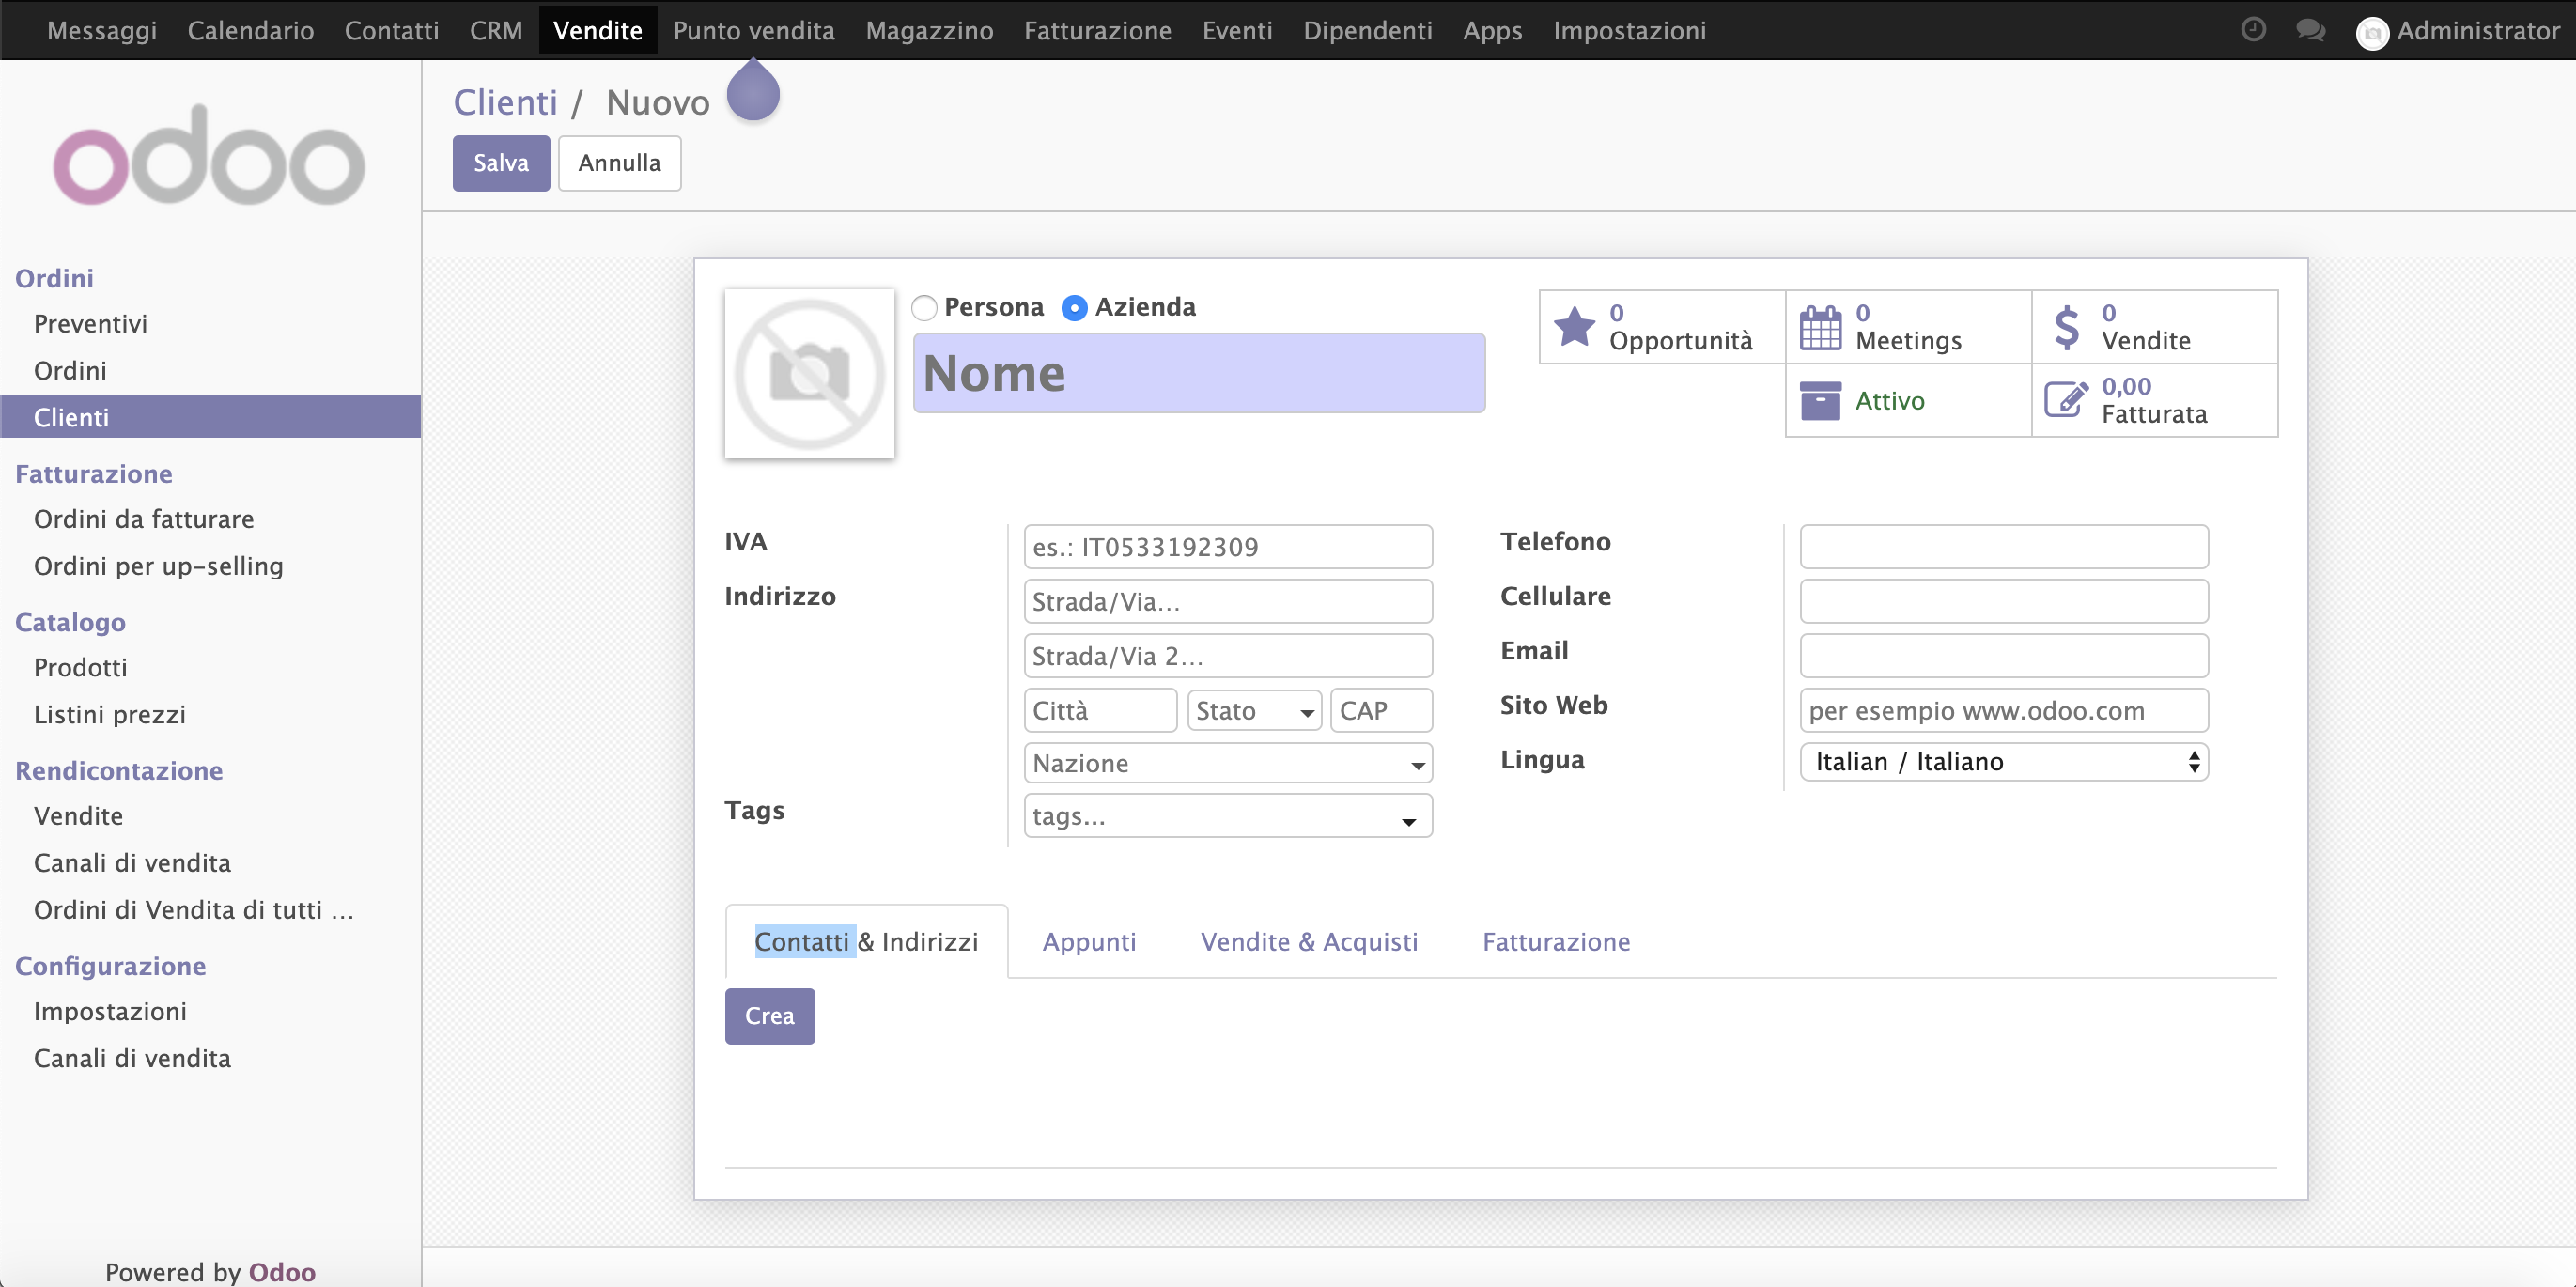
\includegraphics[width=1\linewidth]{figures/empresa}
%	\end{center}
%\end{figure}
%
%\end{frame}


% Gestione imballi

%\begin{frame}{Gestione imballi\scriptsize{(ibg\_packaging)}}
%
%\begin{figure}[H]
%	\begin{center} 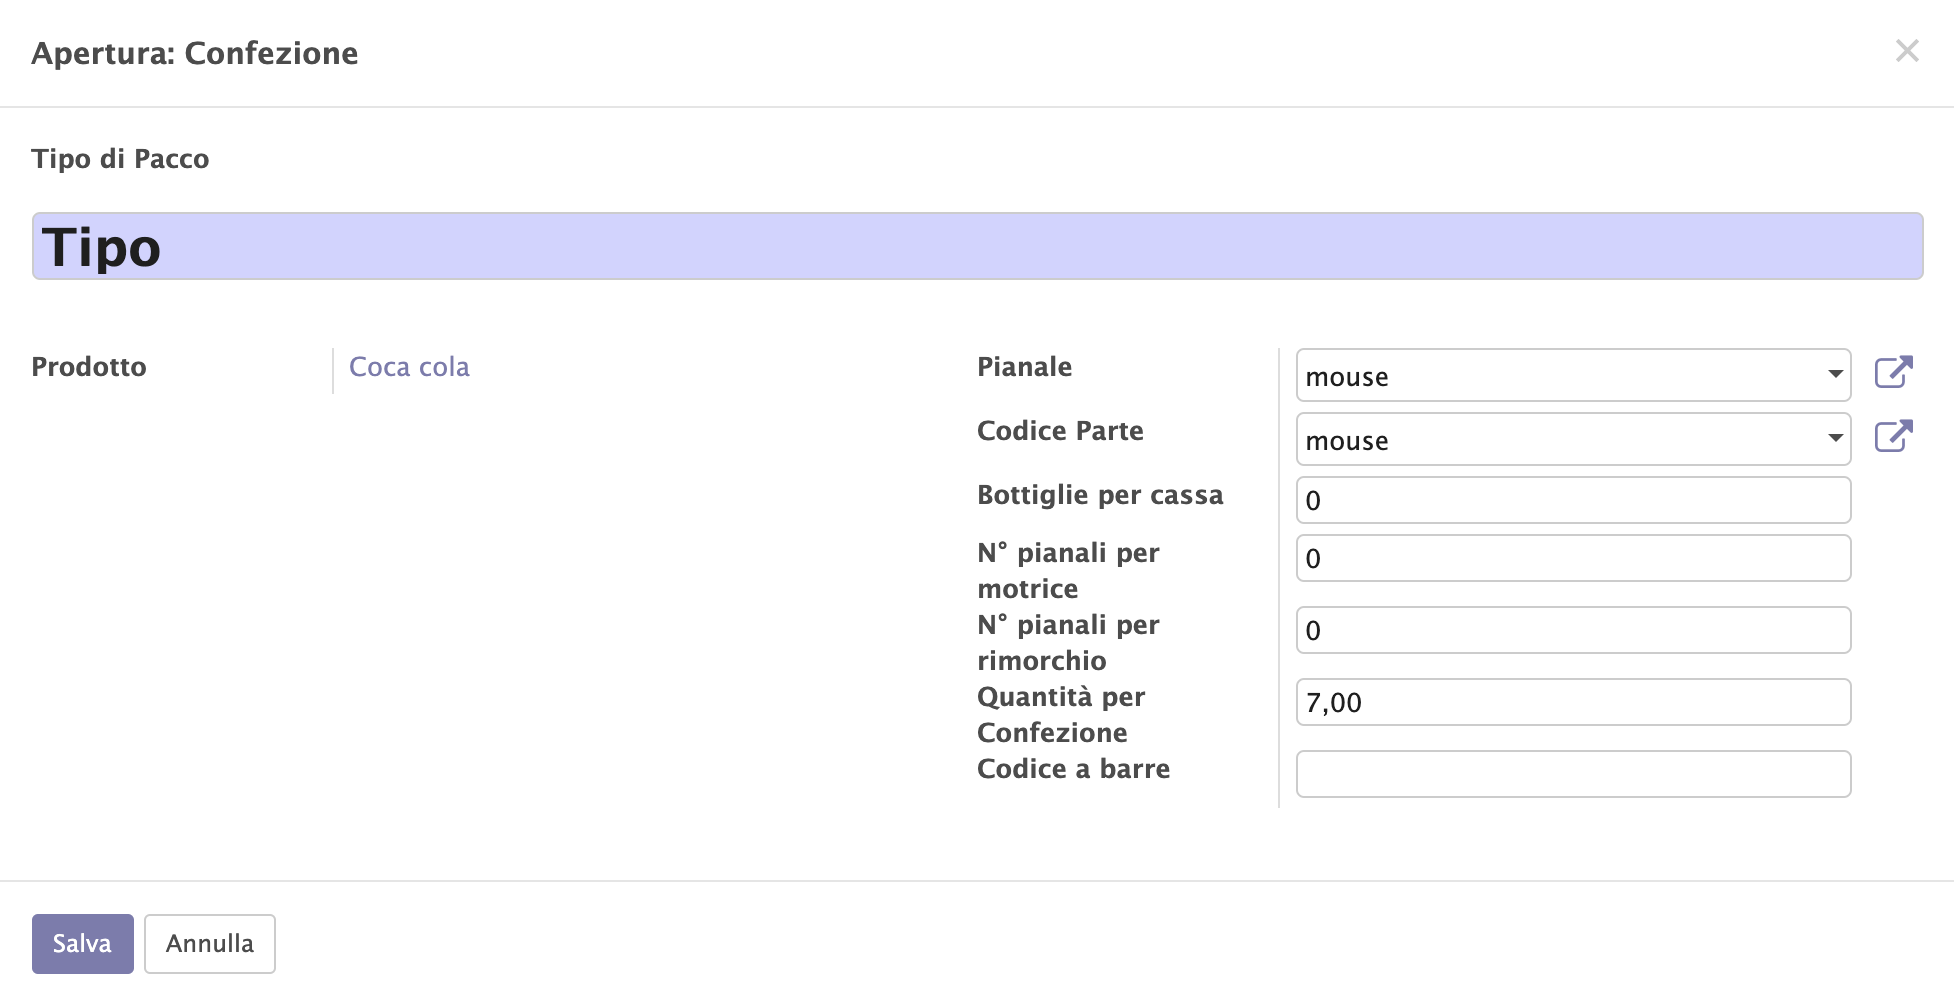
\includegraphics[width=1\linewidth]{figures/package}
%	\end{center}
%\end{figure}
%
%\end{frame}

%\begin{frame}{Gestione imballi}
%
%\begin{figure}[H]
%	\begin{center} 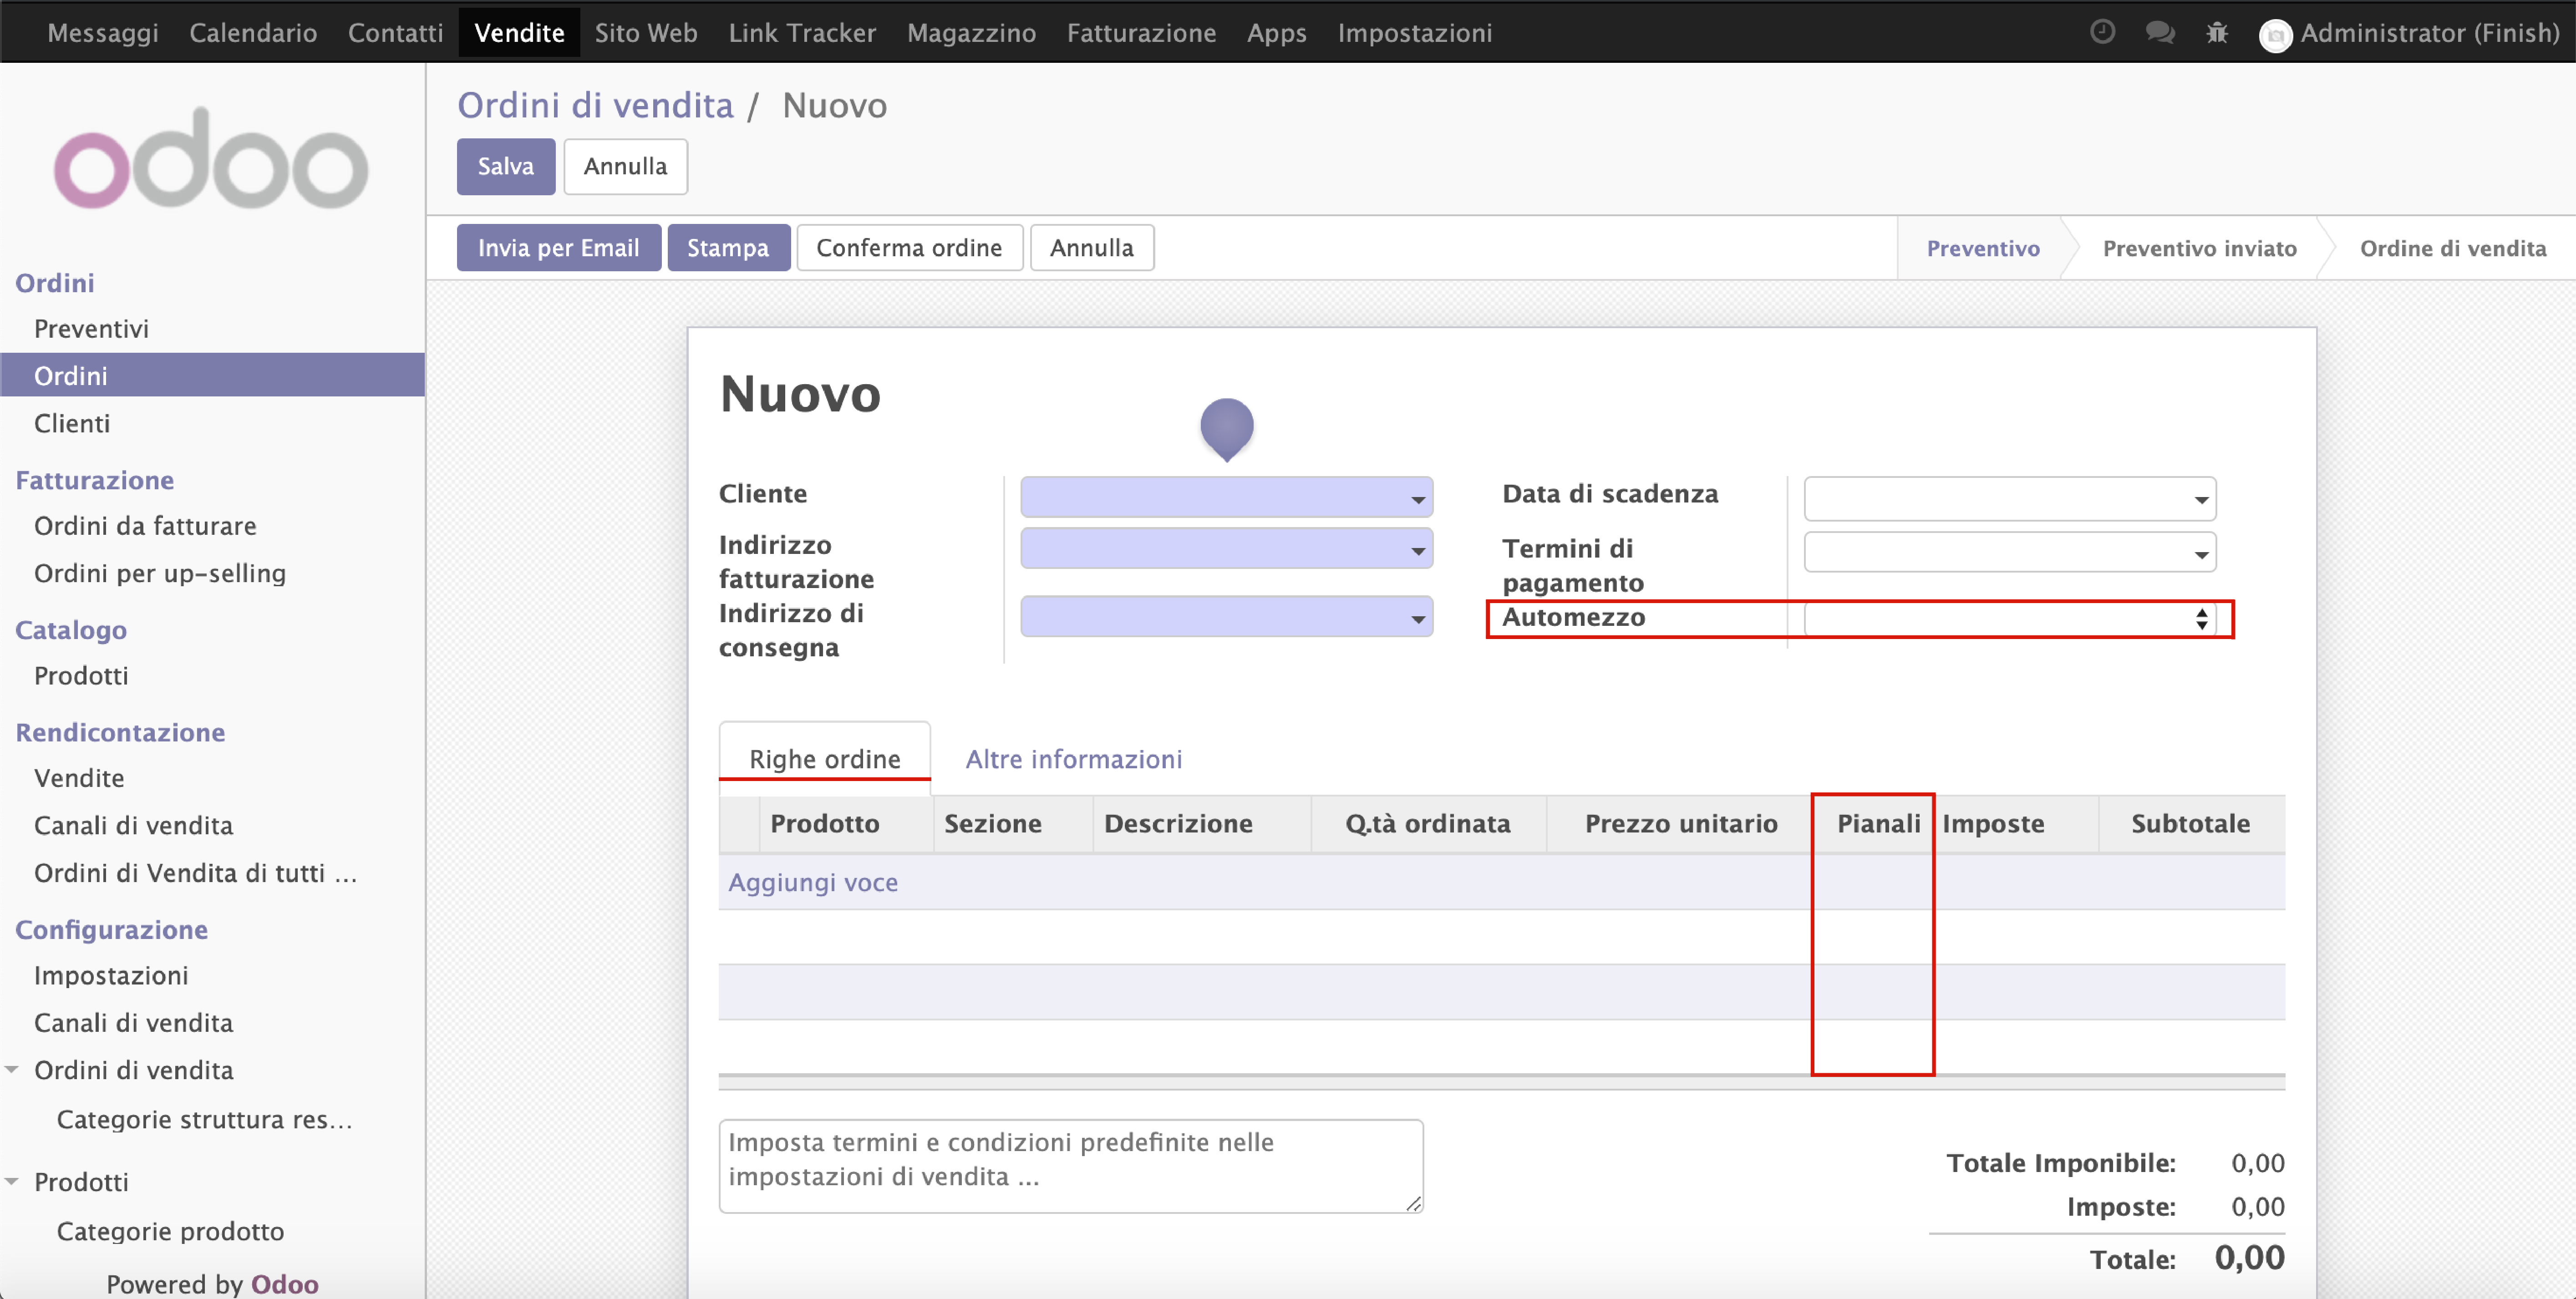
\includegraphics[width=1\linewidth]{figures/pianali}
%	\end{center}
%\end{figure}
%
%\end{frame}


\begin{frame}{Test di sistema e collaudo\scriptsize{(Limite di credito del partner)}}
Per accertare la copertura dei requisiti si \'e ricorso a delle prove pratiche del corretto funzionamento dell’applicazione.

\begin{figure}[H]
	\begin{center} 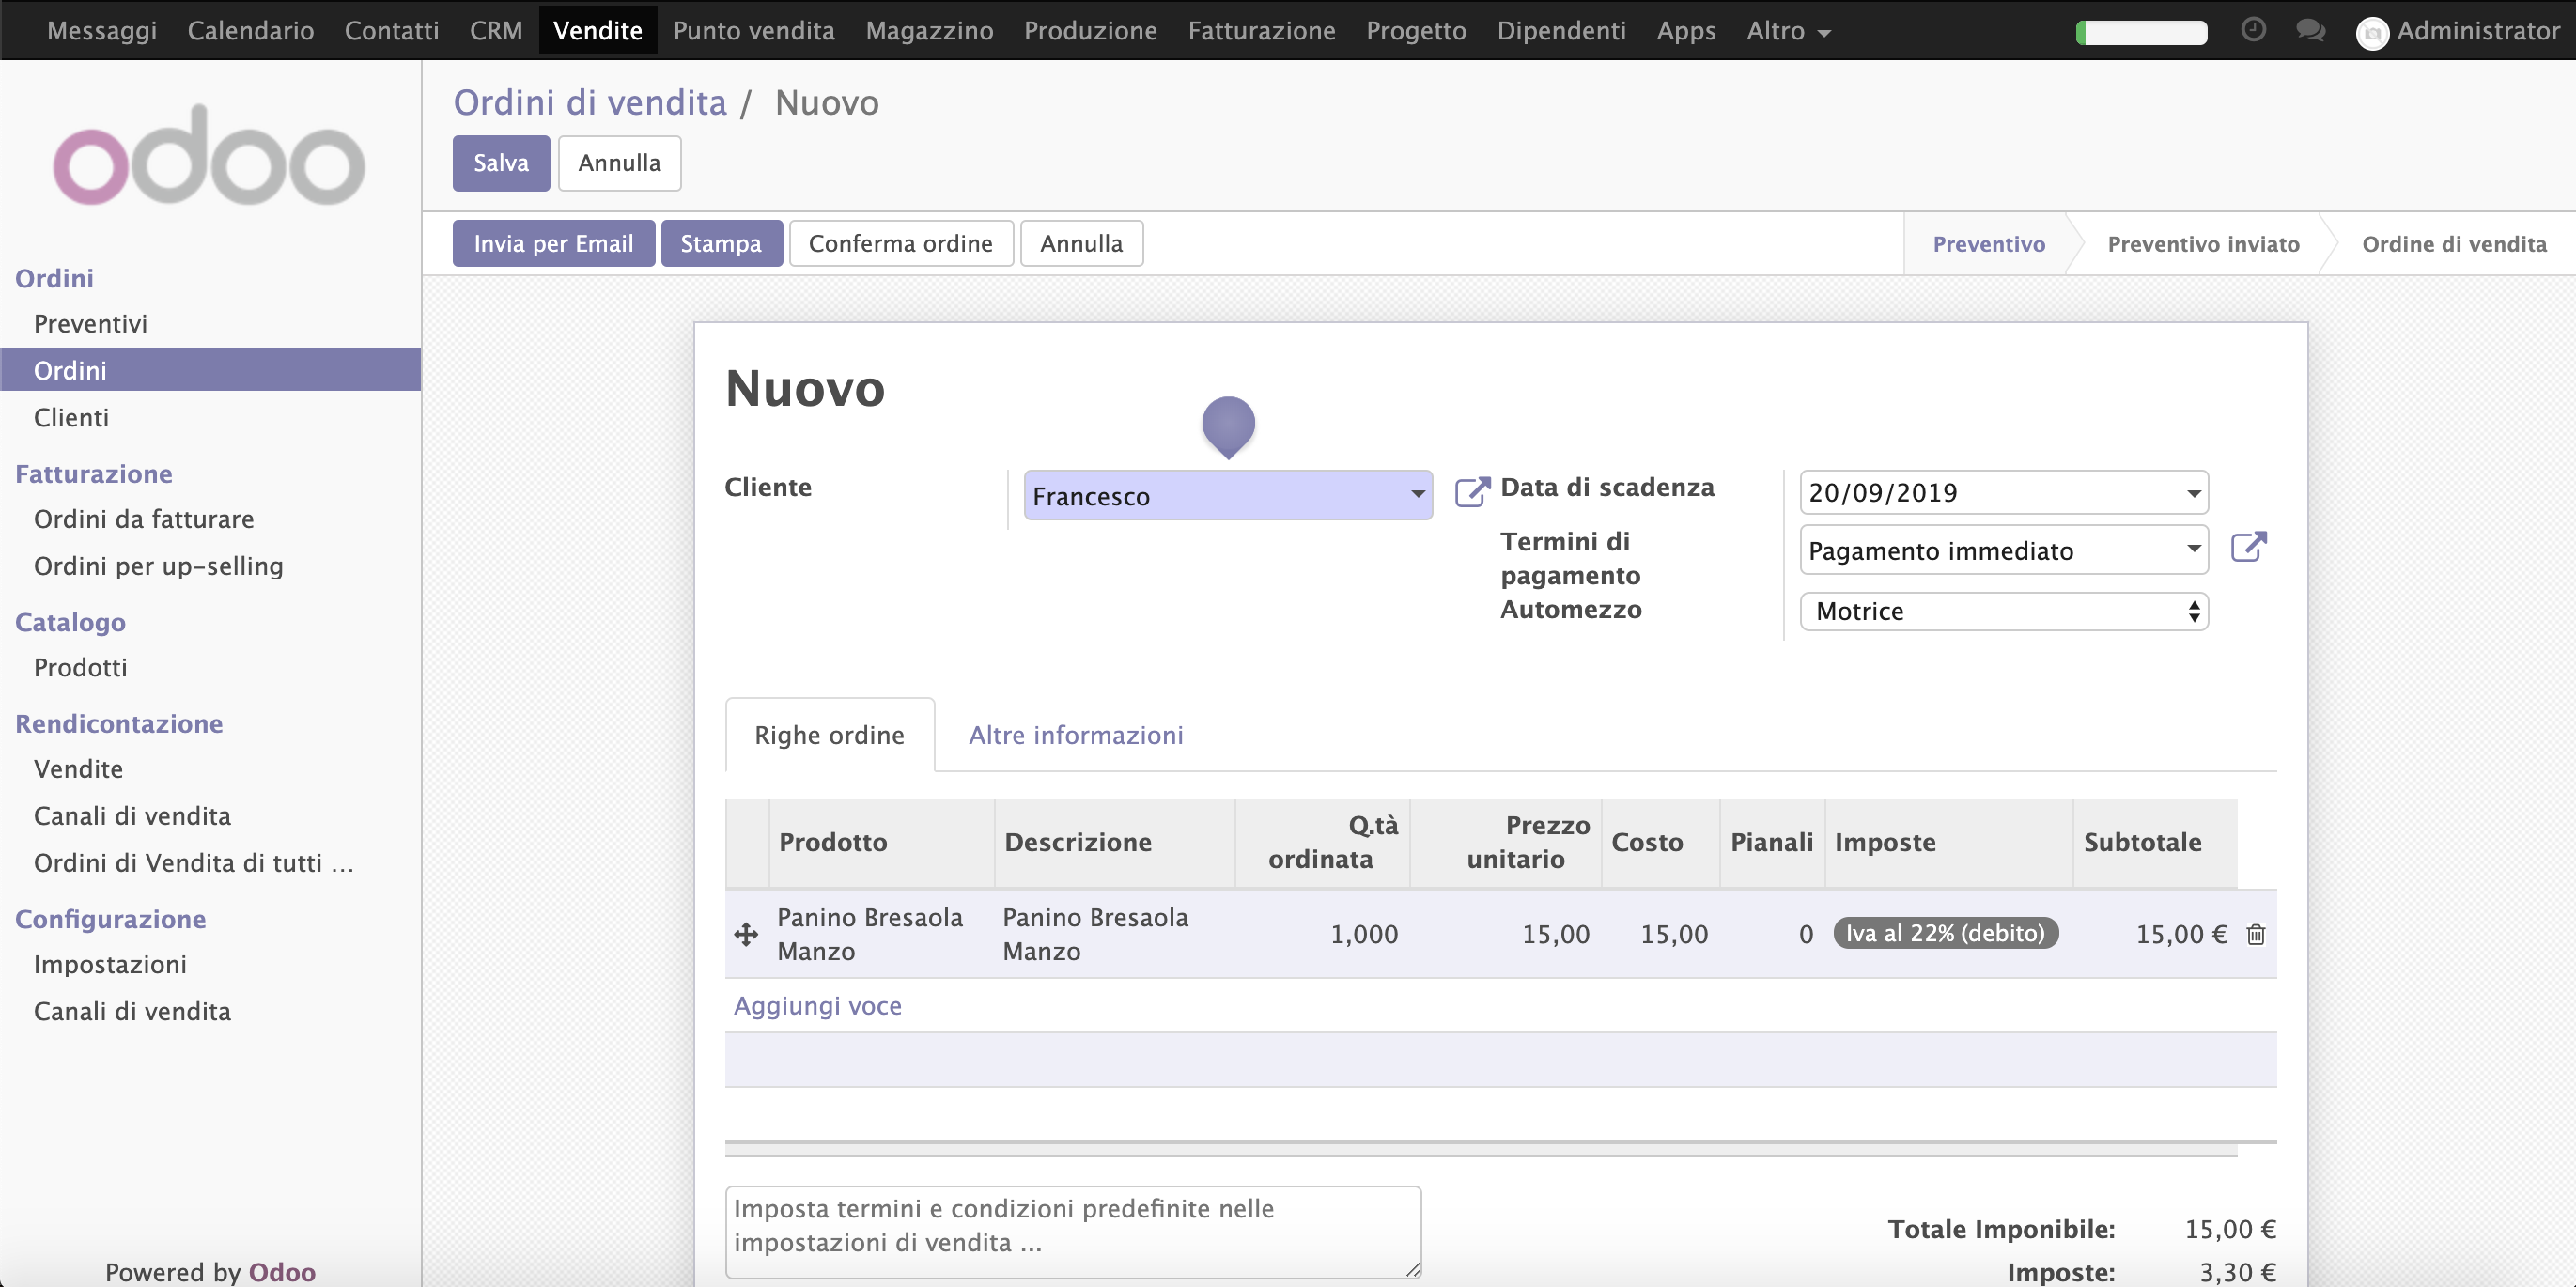
\includegraphics[width=1\linewidth]{figures/limit_home}
	\end{center}
\end{figure}
\end{frame}


\begin{frame}{Test di sistema e collaudo}

\begin{figure}[H]
	\begin{center} 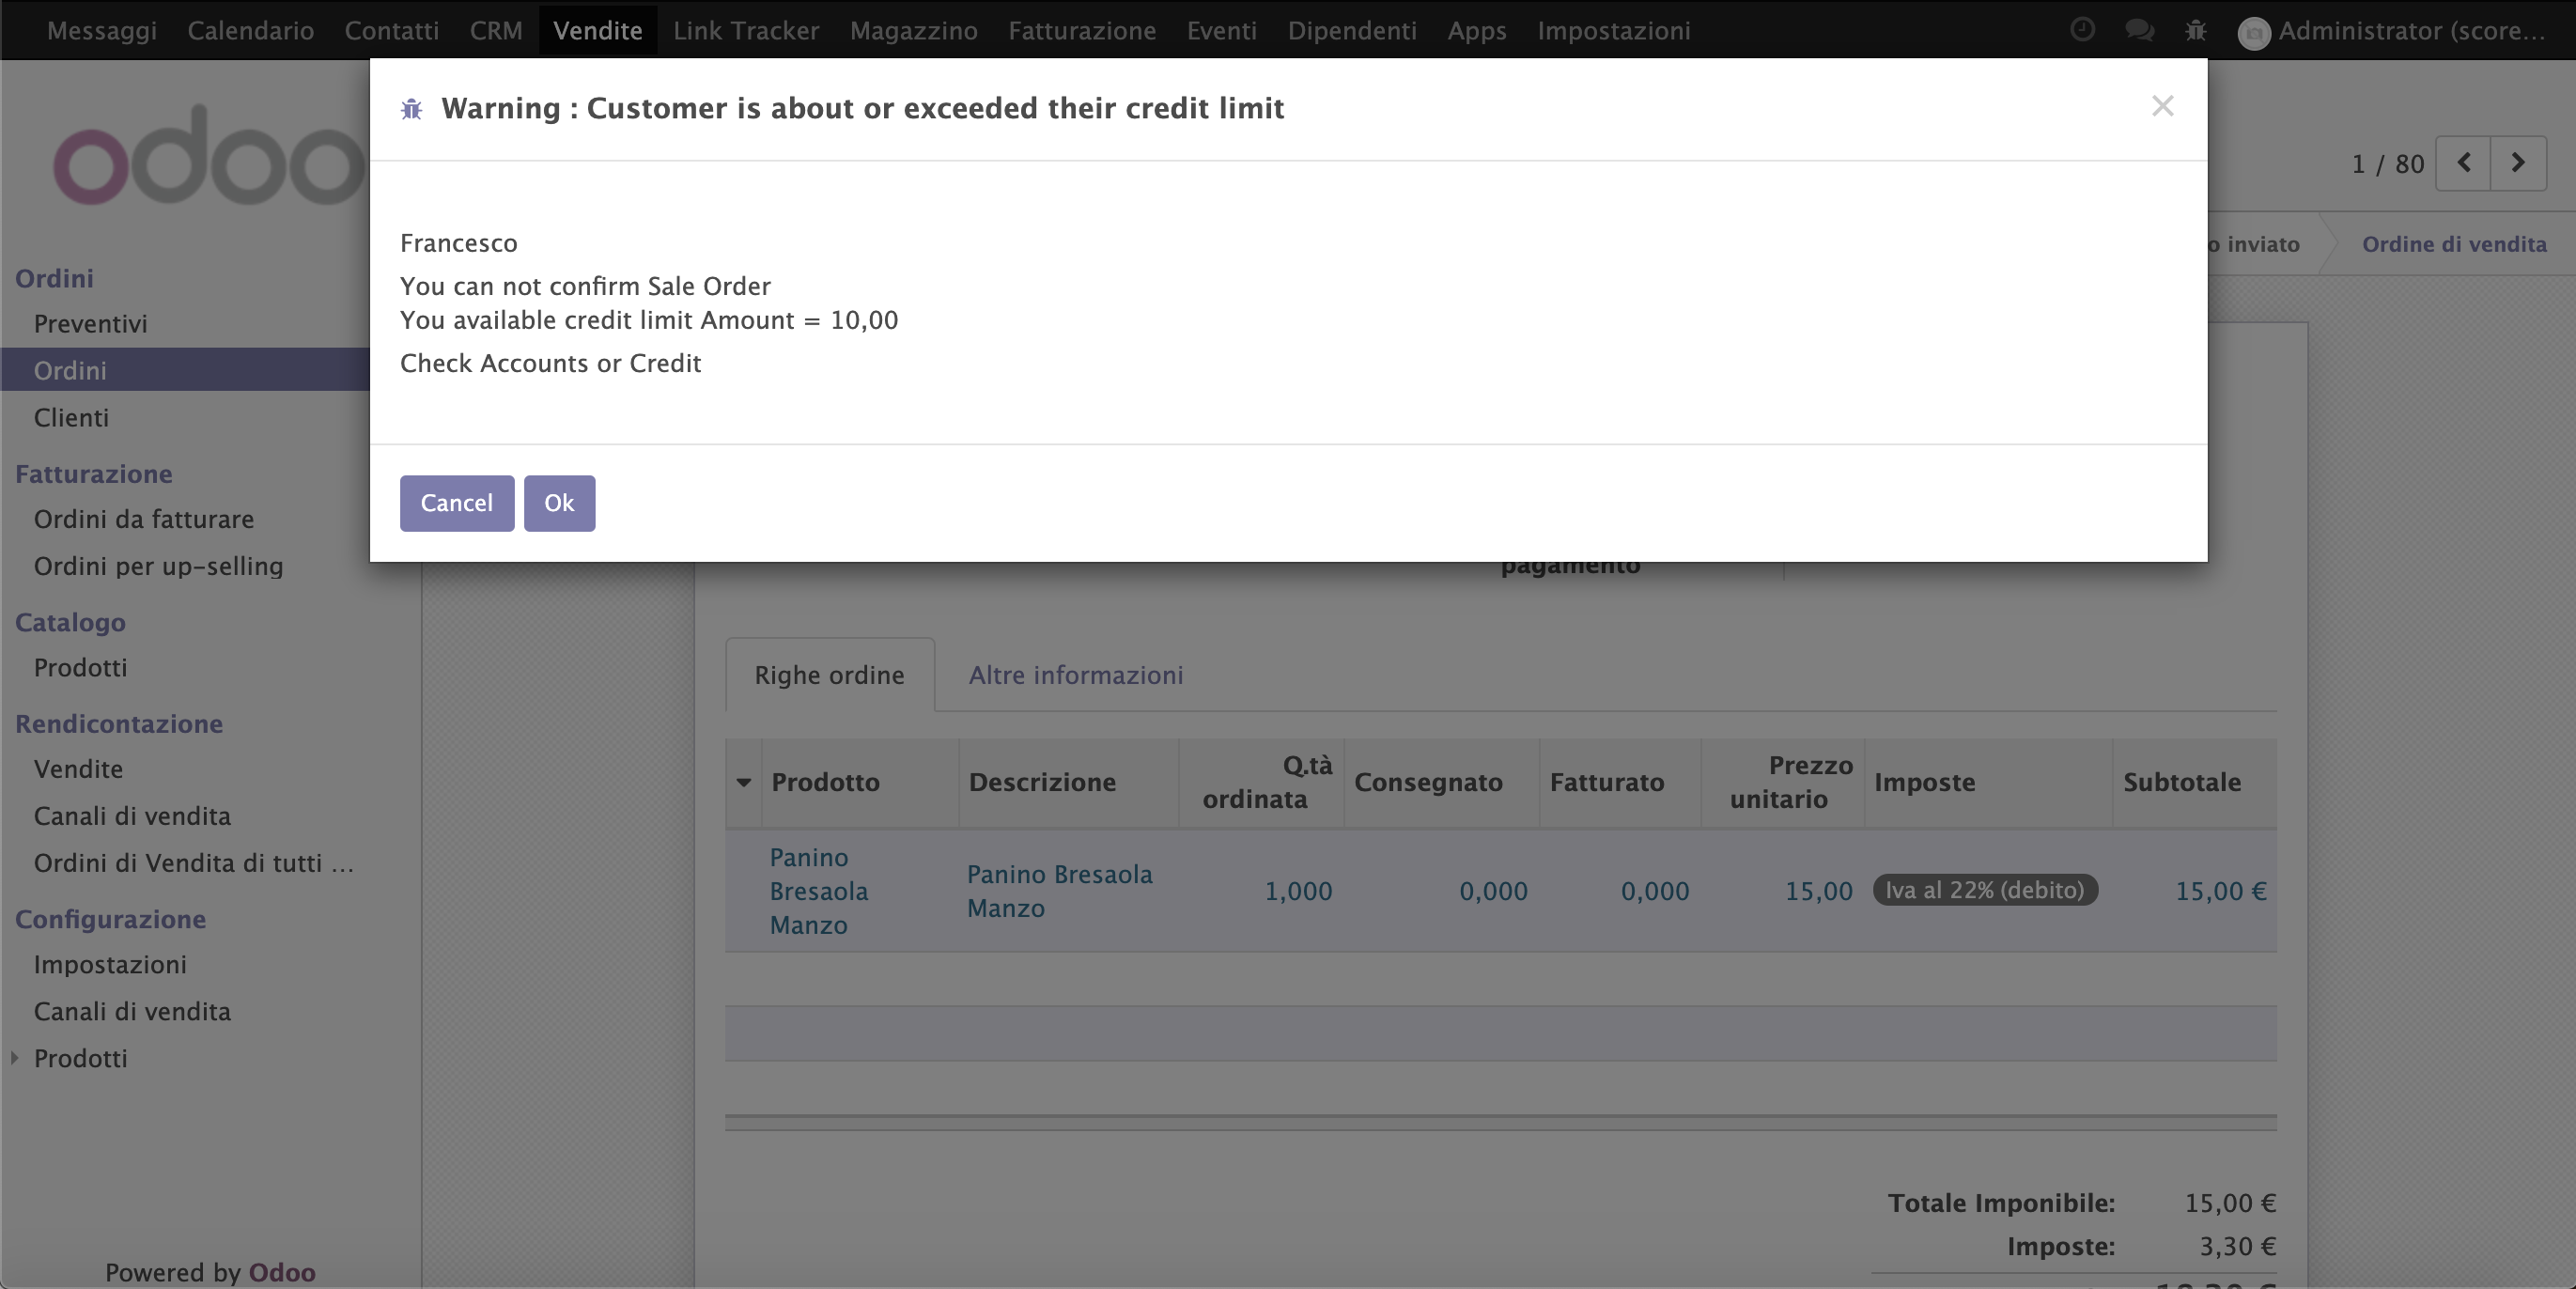
\includegraphics[width=0.95\linewidth]{figures/check_limit}
	\end{center}
\end{figure}
Inoltre verrà inviata una mail al direttore commerciale, che sar\'a informato dell'errore al relativo ordine di vendita.
\end{frame}


\begin{frame}{Test di sistema e collaudo}

\begin{figure}[H]
	\begin{center} 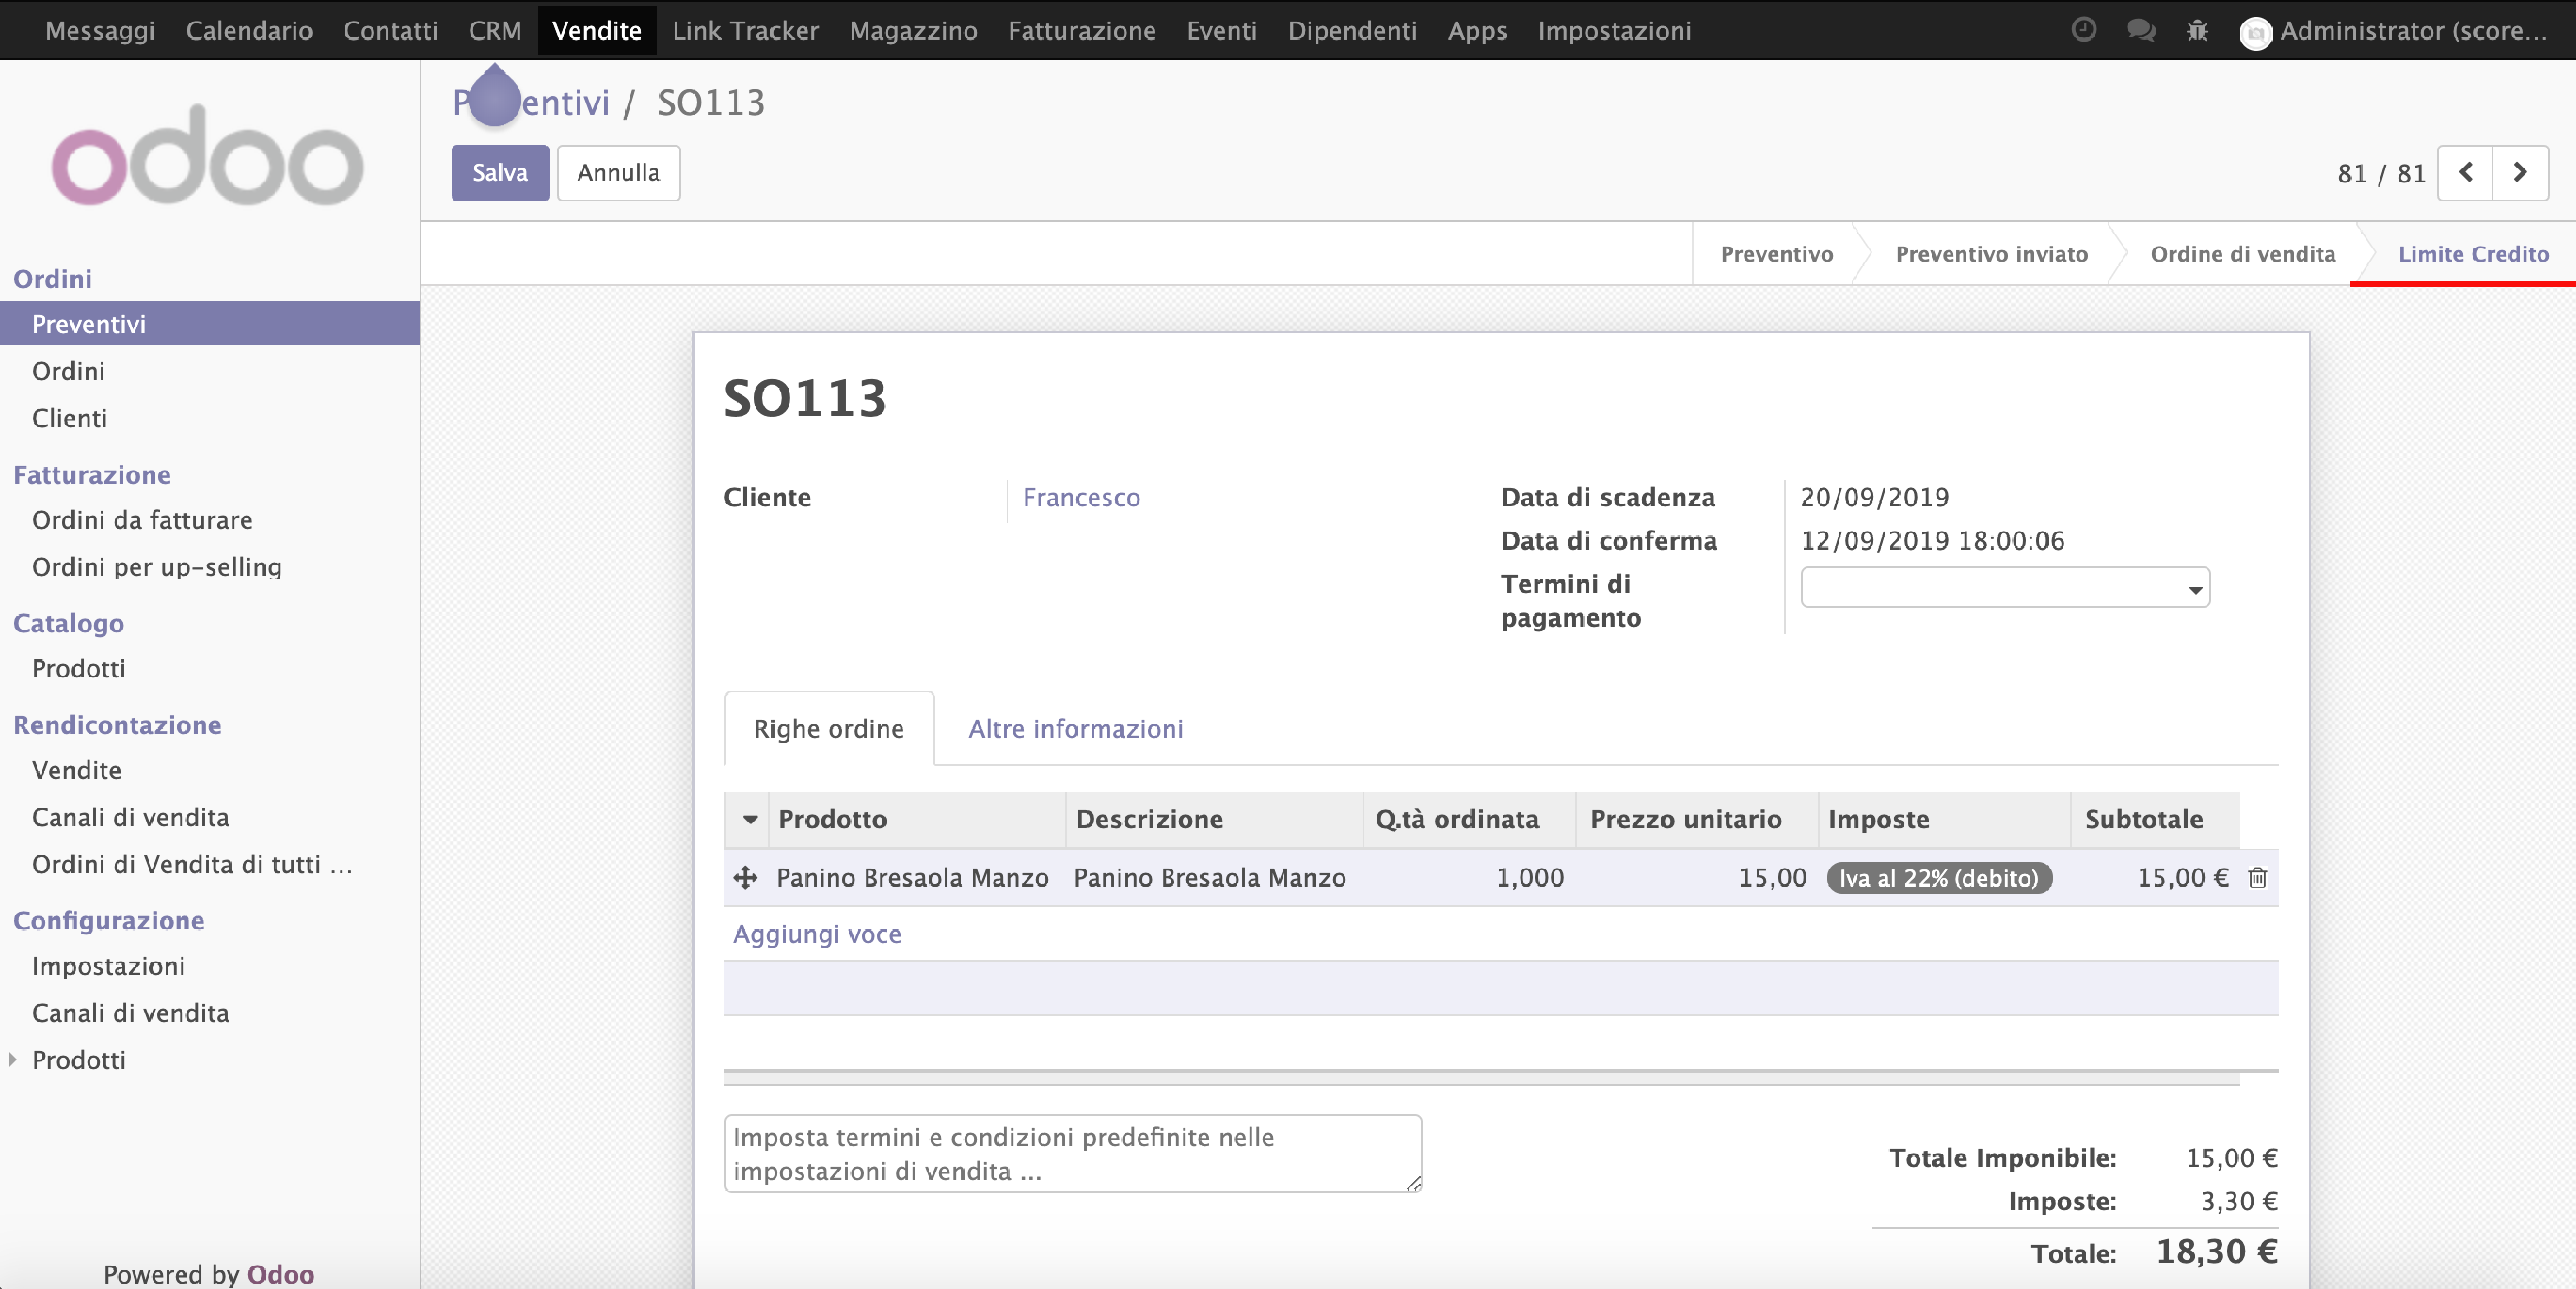
\includegraphics[width=1\linewidth]{figures/second_test}
	\end{center}
\end{figure}

\end{frame}

%\begin{frame}{Test di sistema e collaudo\scriptsize{(Canali di vendita)}}
%
%\begin{figure}[H]
%	\begin{center} 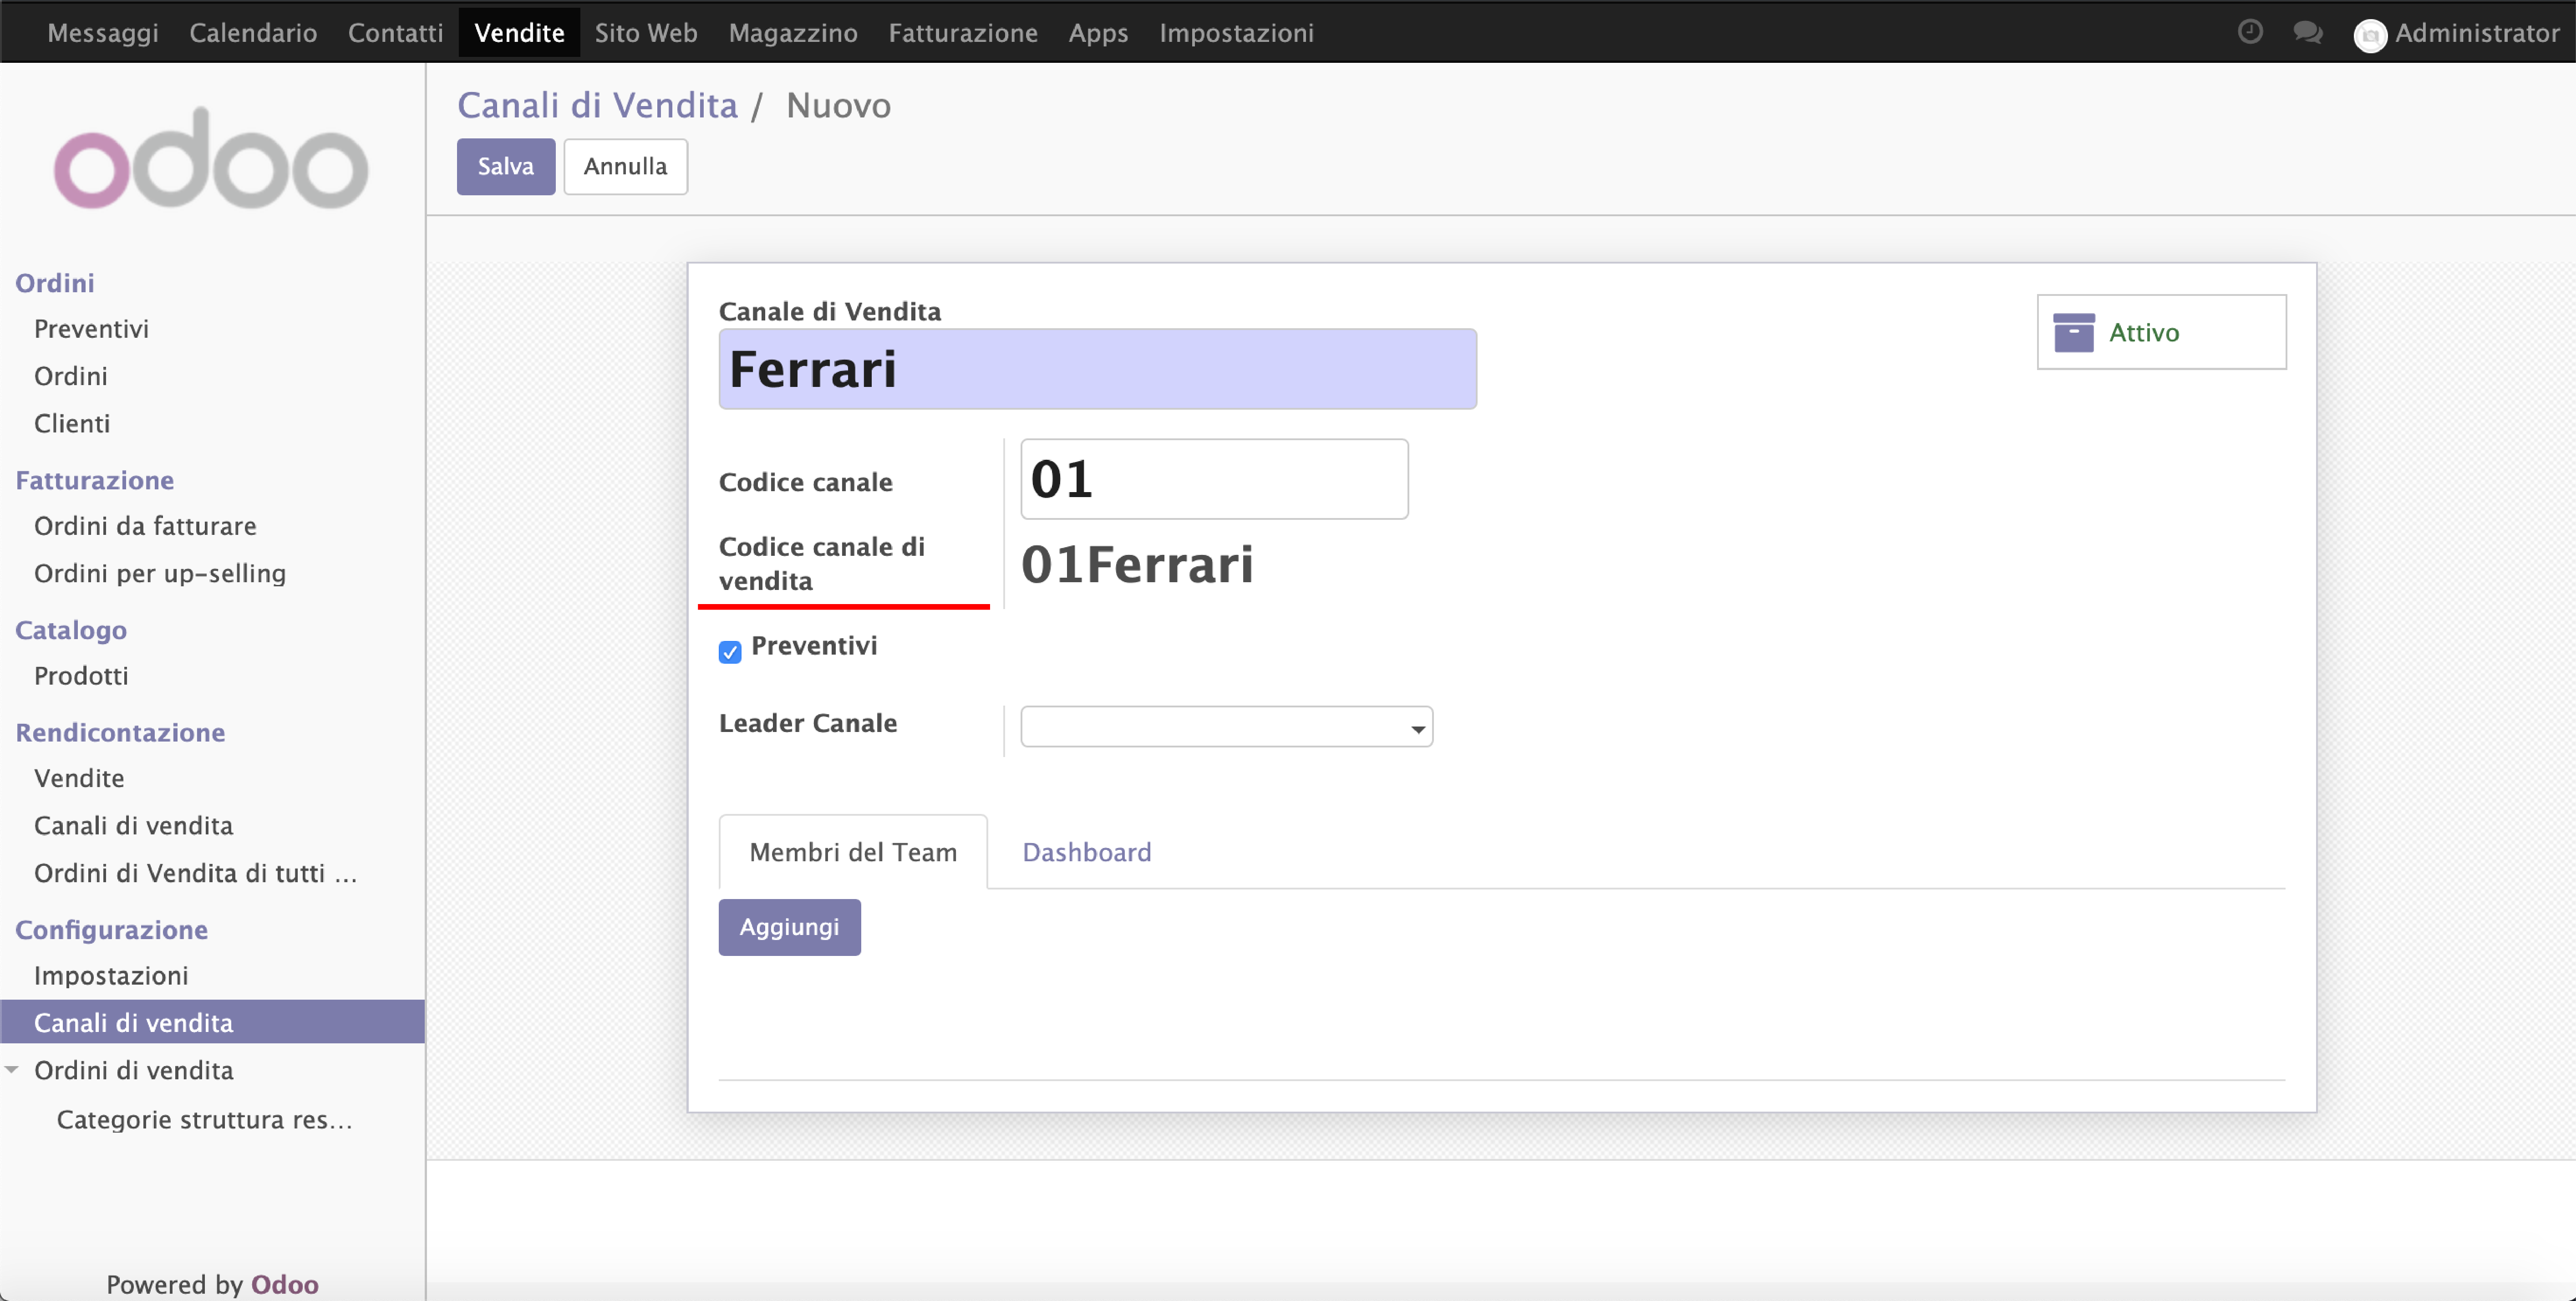
\includegraphics[width=1\linewidth]{figures/fourth_test}
%	\end{center}
%\end{figure}
%
%\end{frame}

%
%		Test di sistema e collaudo Gestione imballi
%
%\begin{frame}{Test di sistema e collaudo\scriptsize{(Gestione imballi)}}
%
%
%\begin{figure}[H]
%	\begin{center} 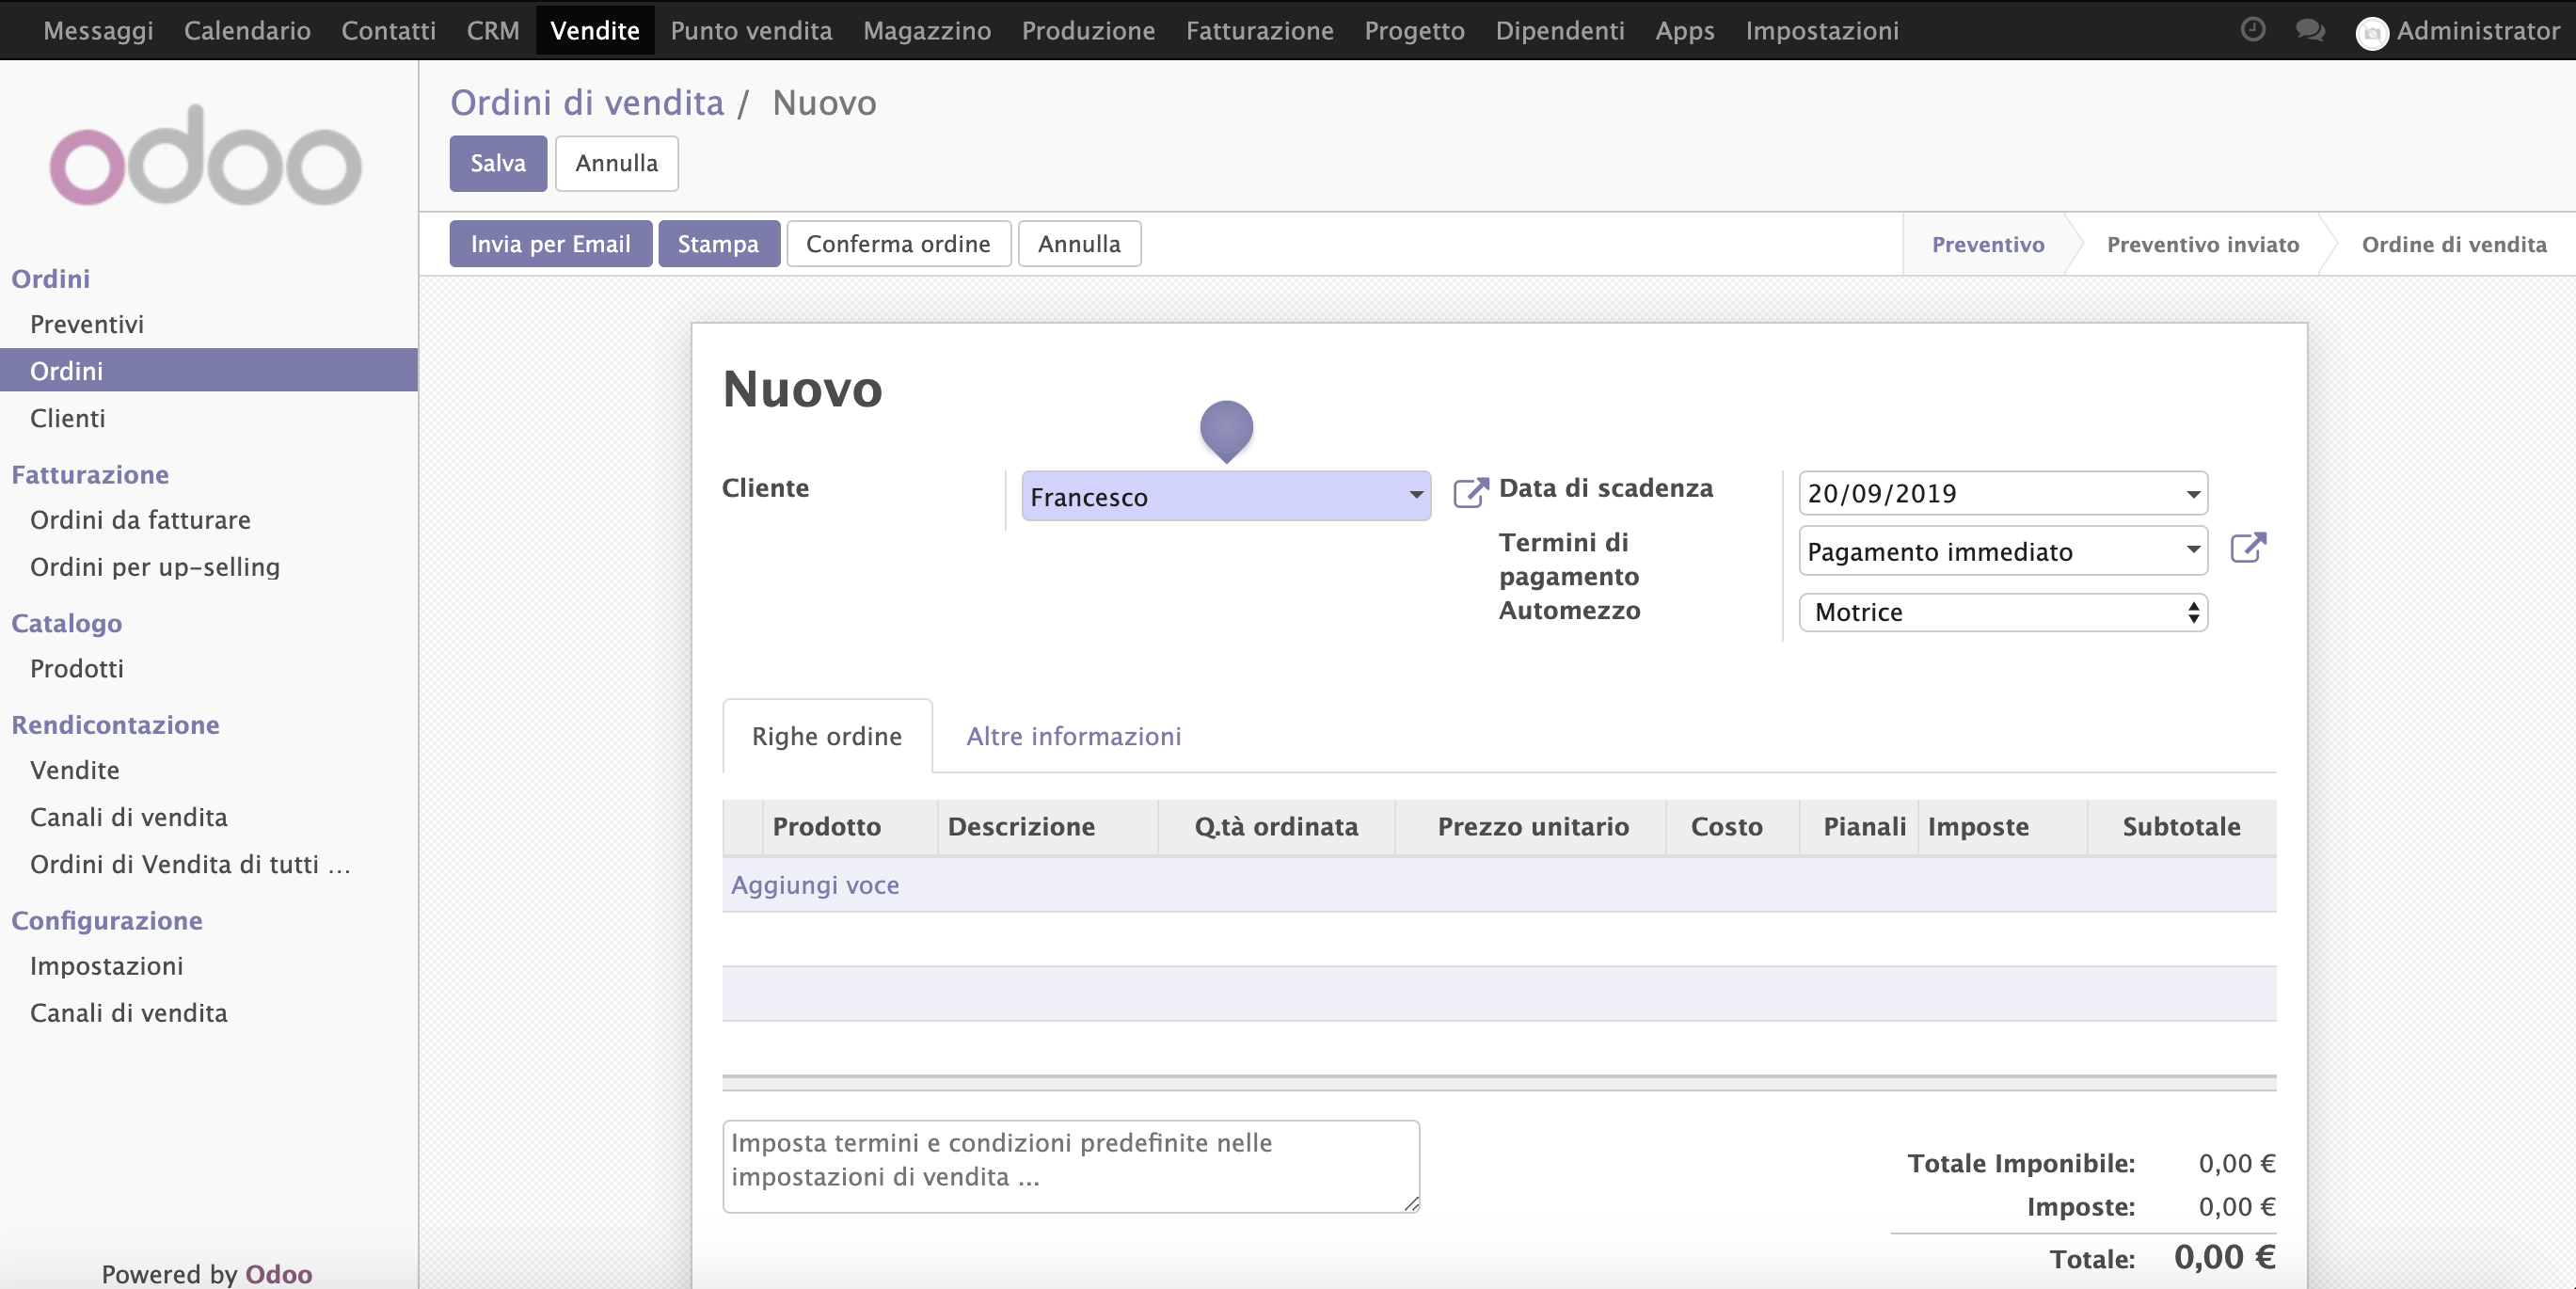
\includegraphics[width=1\linewidth]{figures/one}
%	\end{center}
%\end{figure}
%
%\end{frame}


%\begin{frame}{Test di sistema e collaudo}
%
%
%\begin{figure}[H]
%	\begin{center} 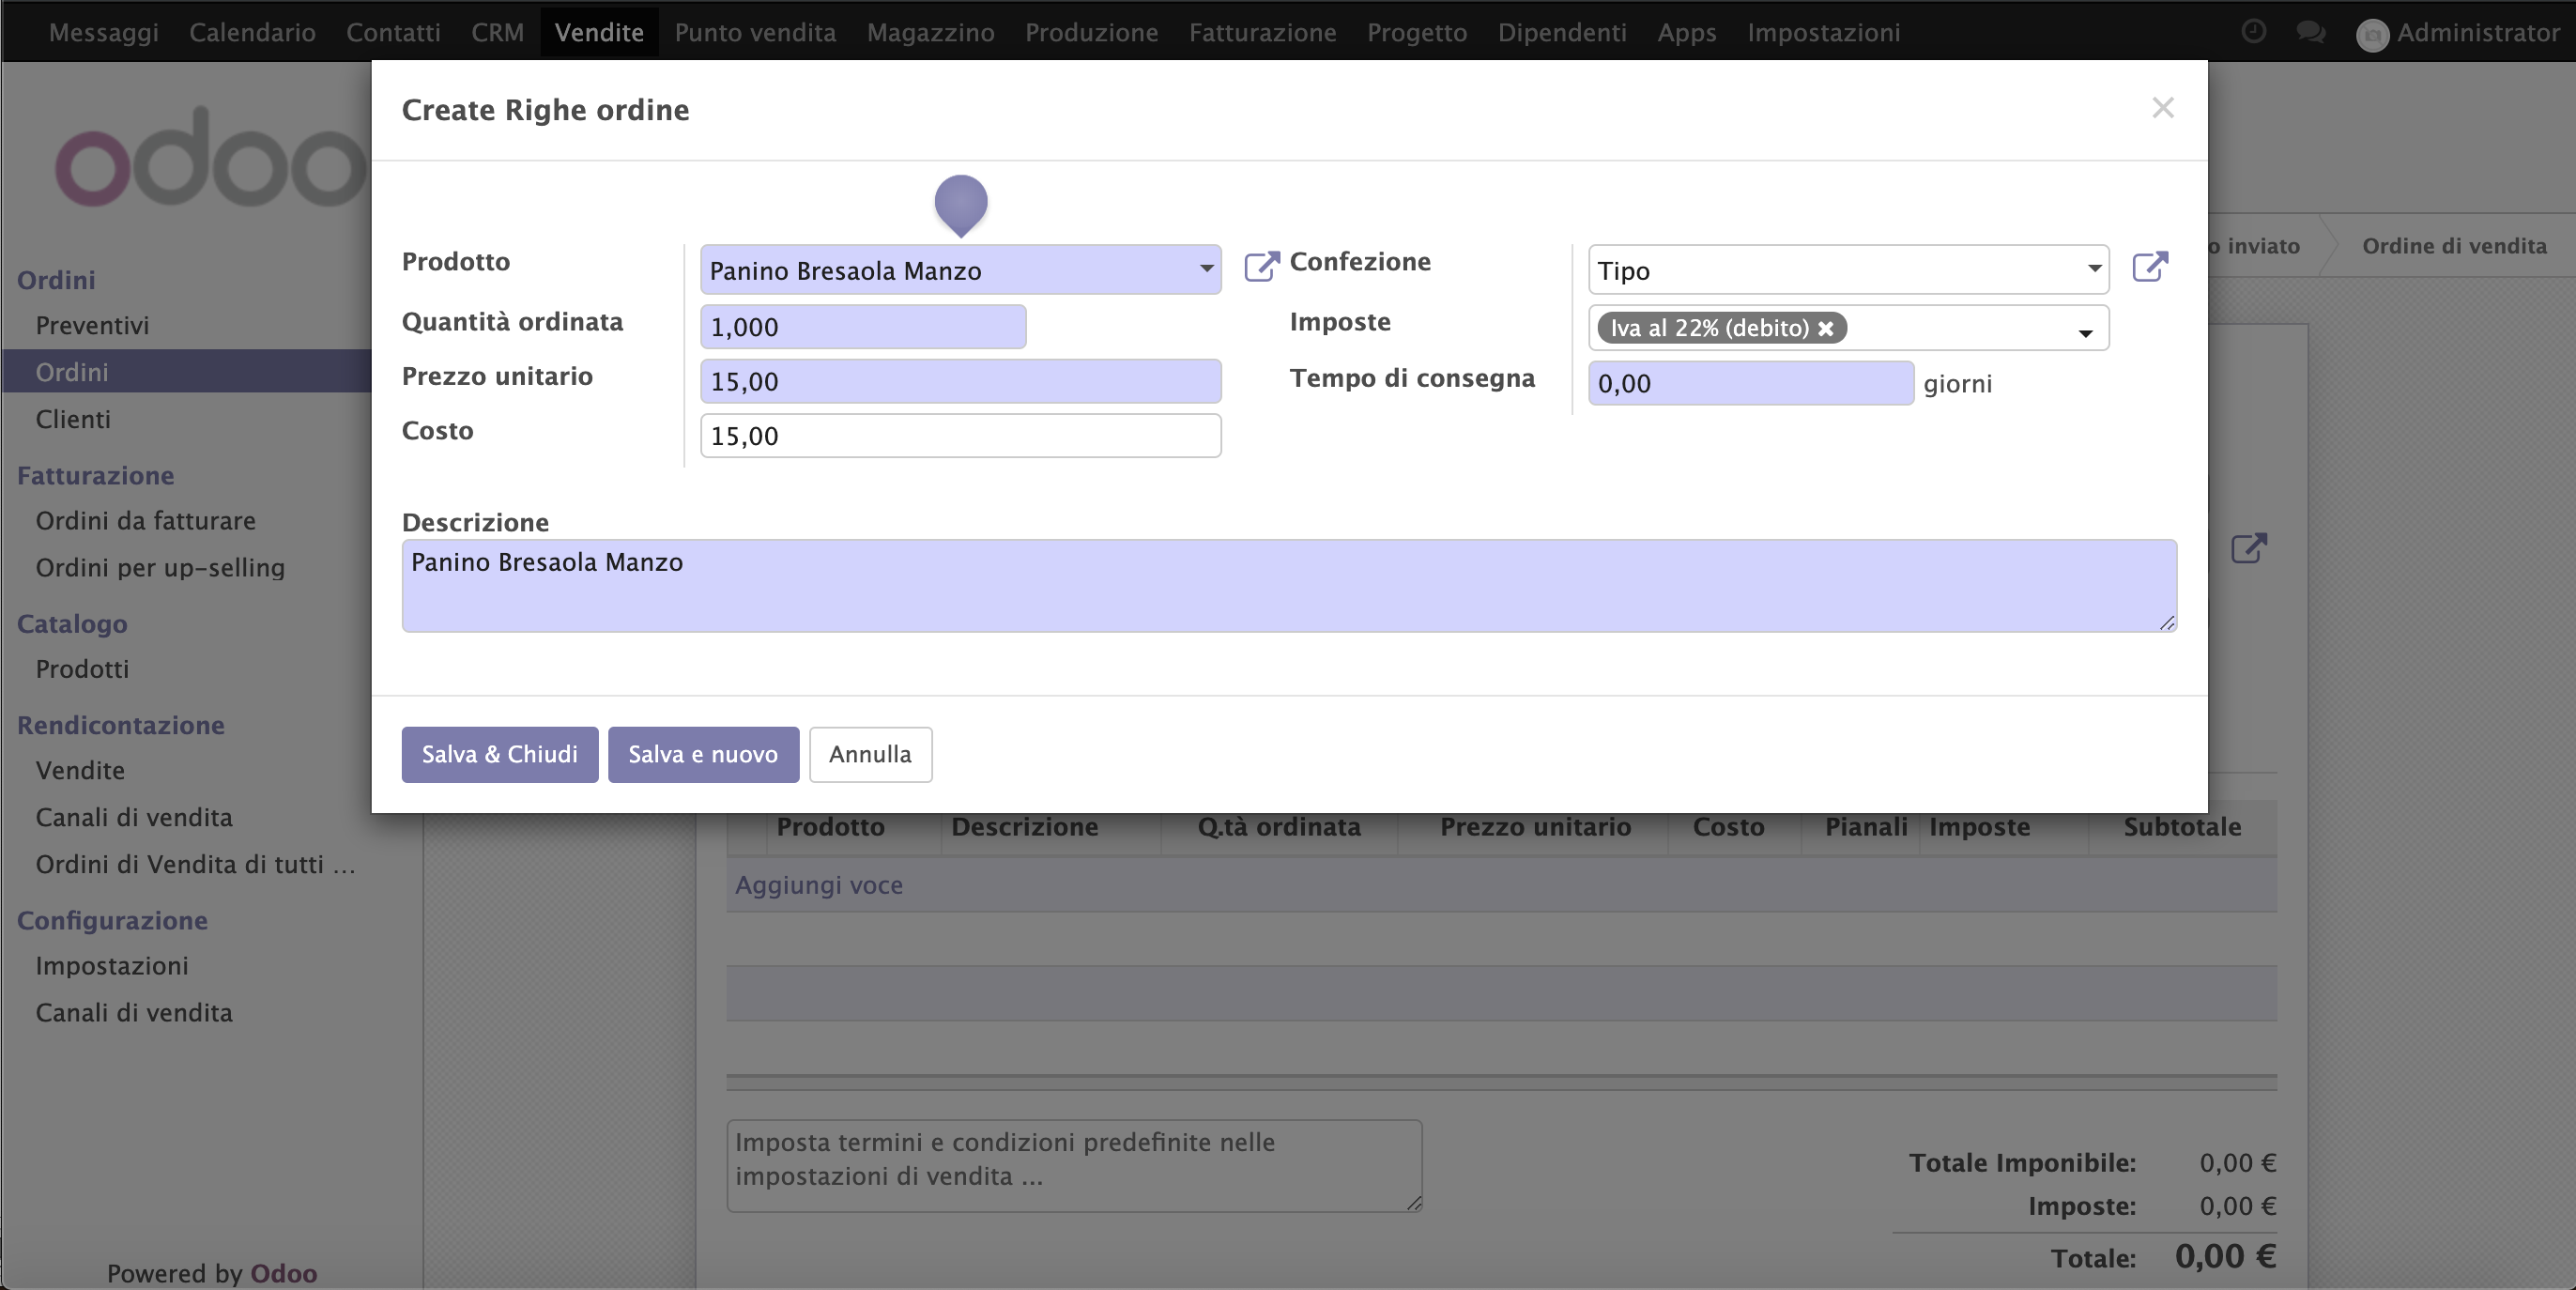
\includegraphics[width=1\linewidth]{figures/panini}
%	\end{center}
%\end{figure}
%
%\end{frame}



%\begin{frame}{Test di sistema e collaudo}
%\begin{figure}[H]
%	\begin{center} 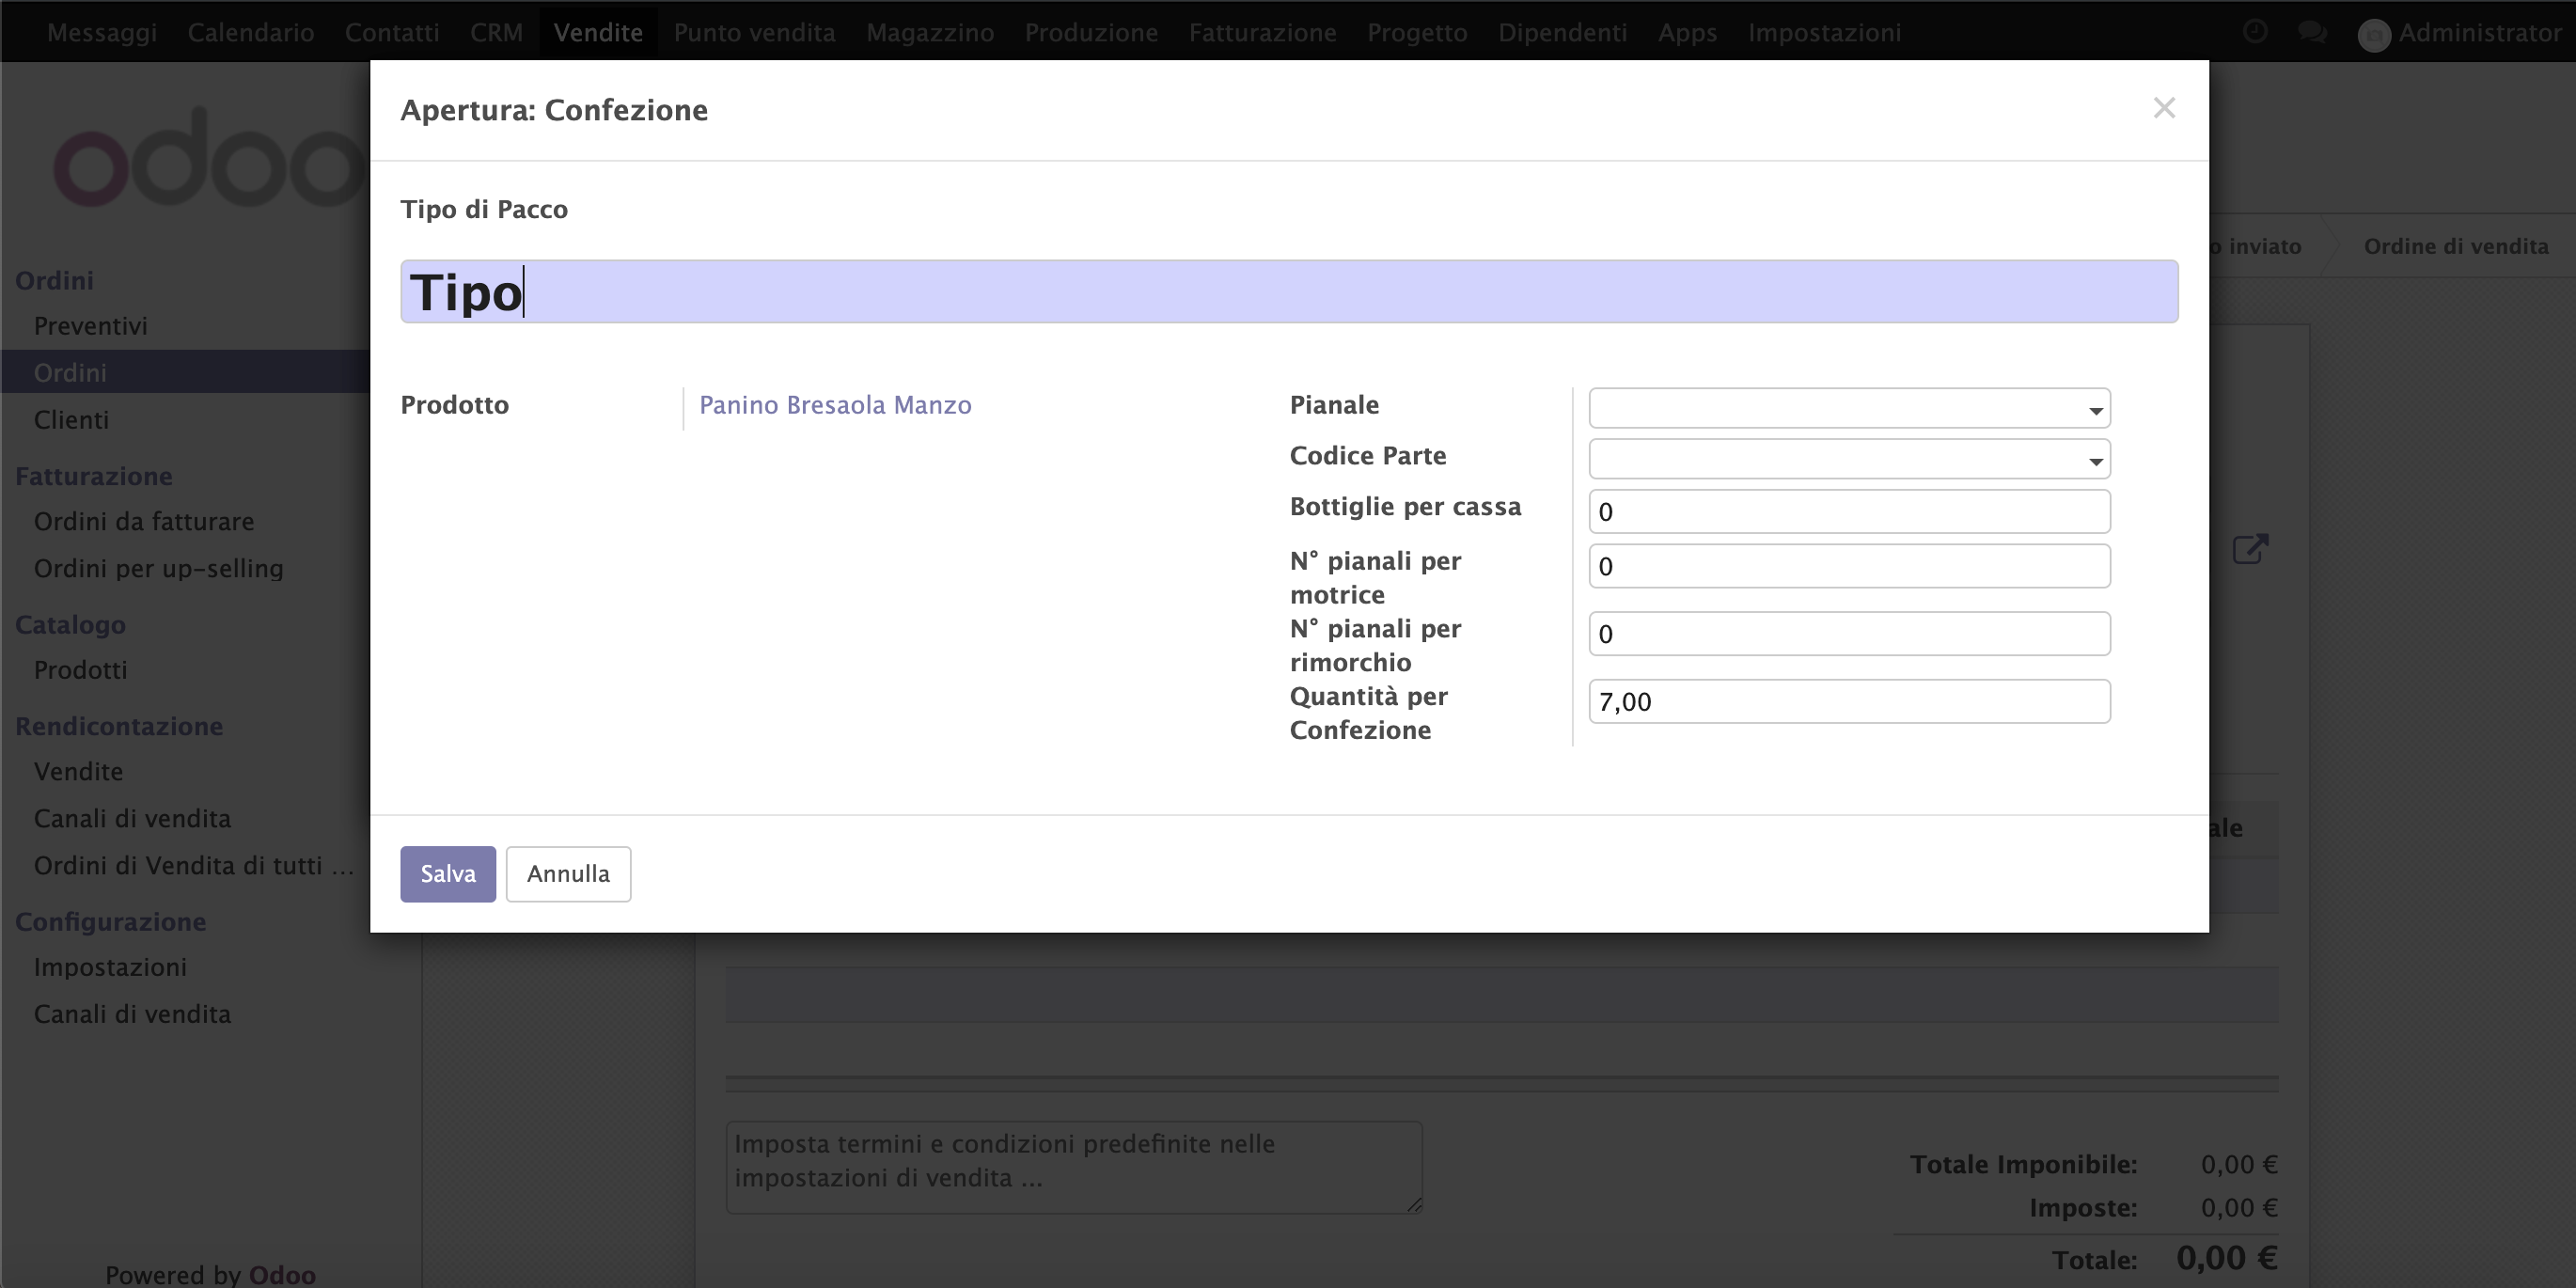
\includegraphics[width=1\linewidth]{figures/imballo}
%	\end{center}
%\end{figure}
%
%\end{frame}
%
%
%\begin{frame}{Test di sistema e collaudo}
%’Pianali’: \'e dato dal rapporto fra Quantit\'a ordinata (20) / Quantit\'a per confezione (7) = 2,85.
%
%\begin{figure}[H]
%	\begin{center} 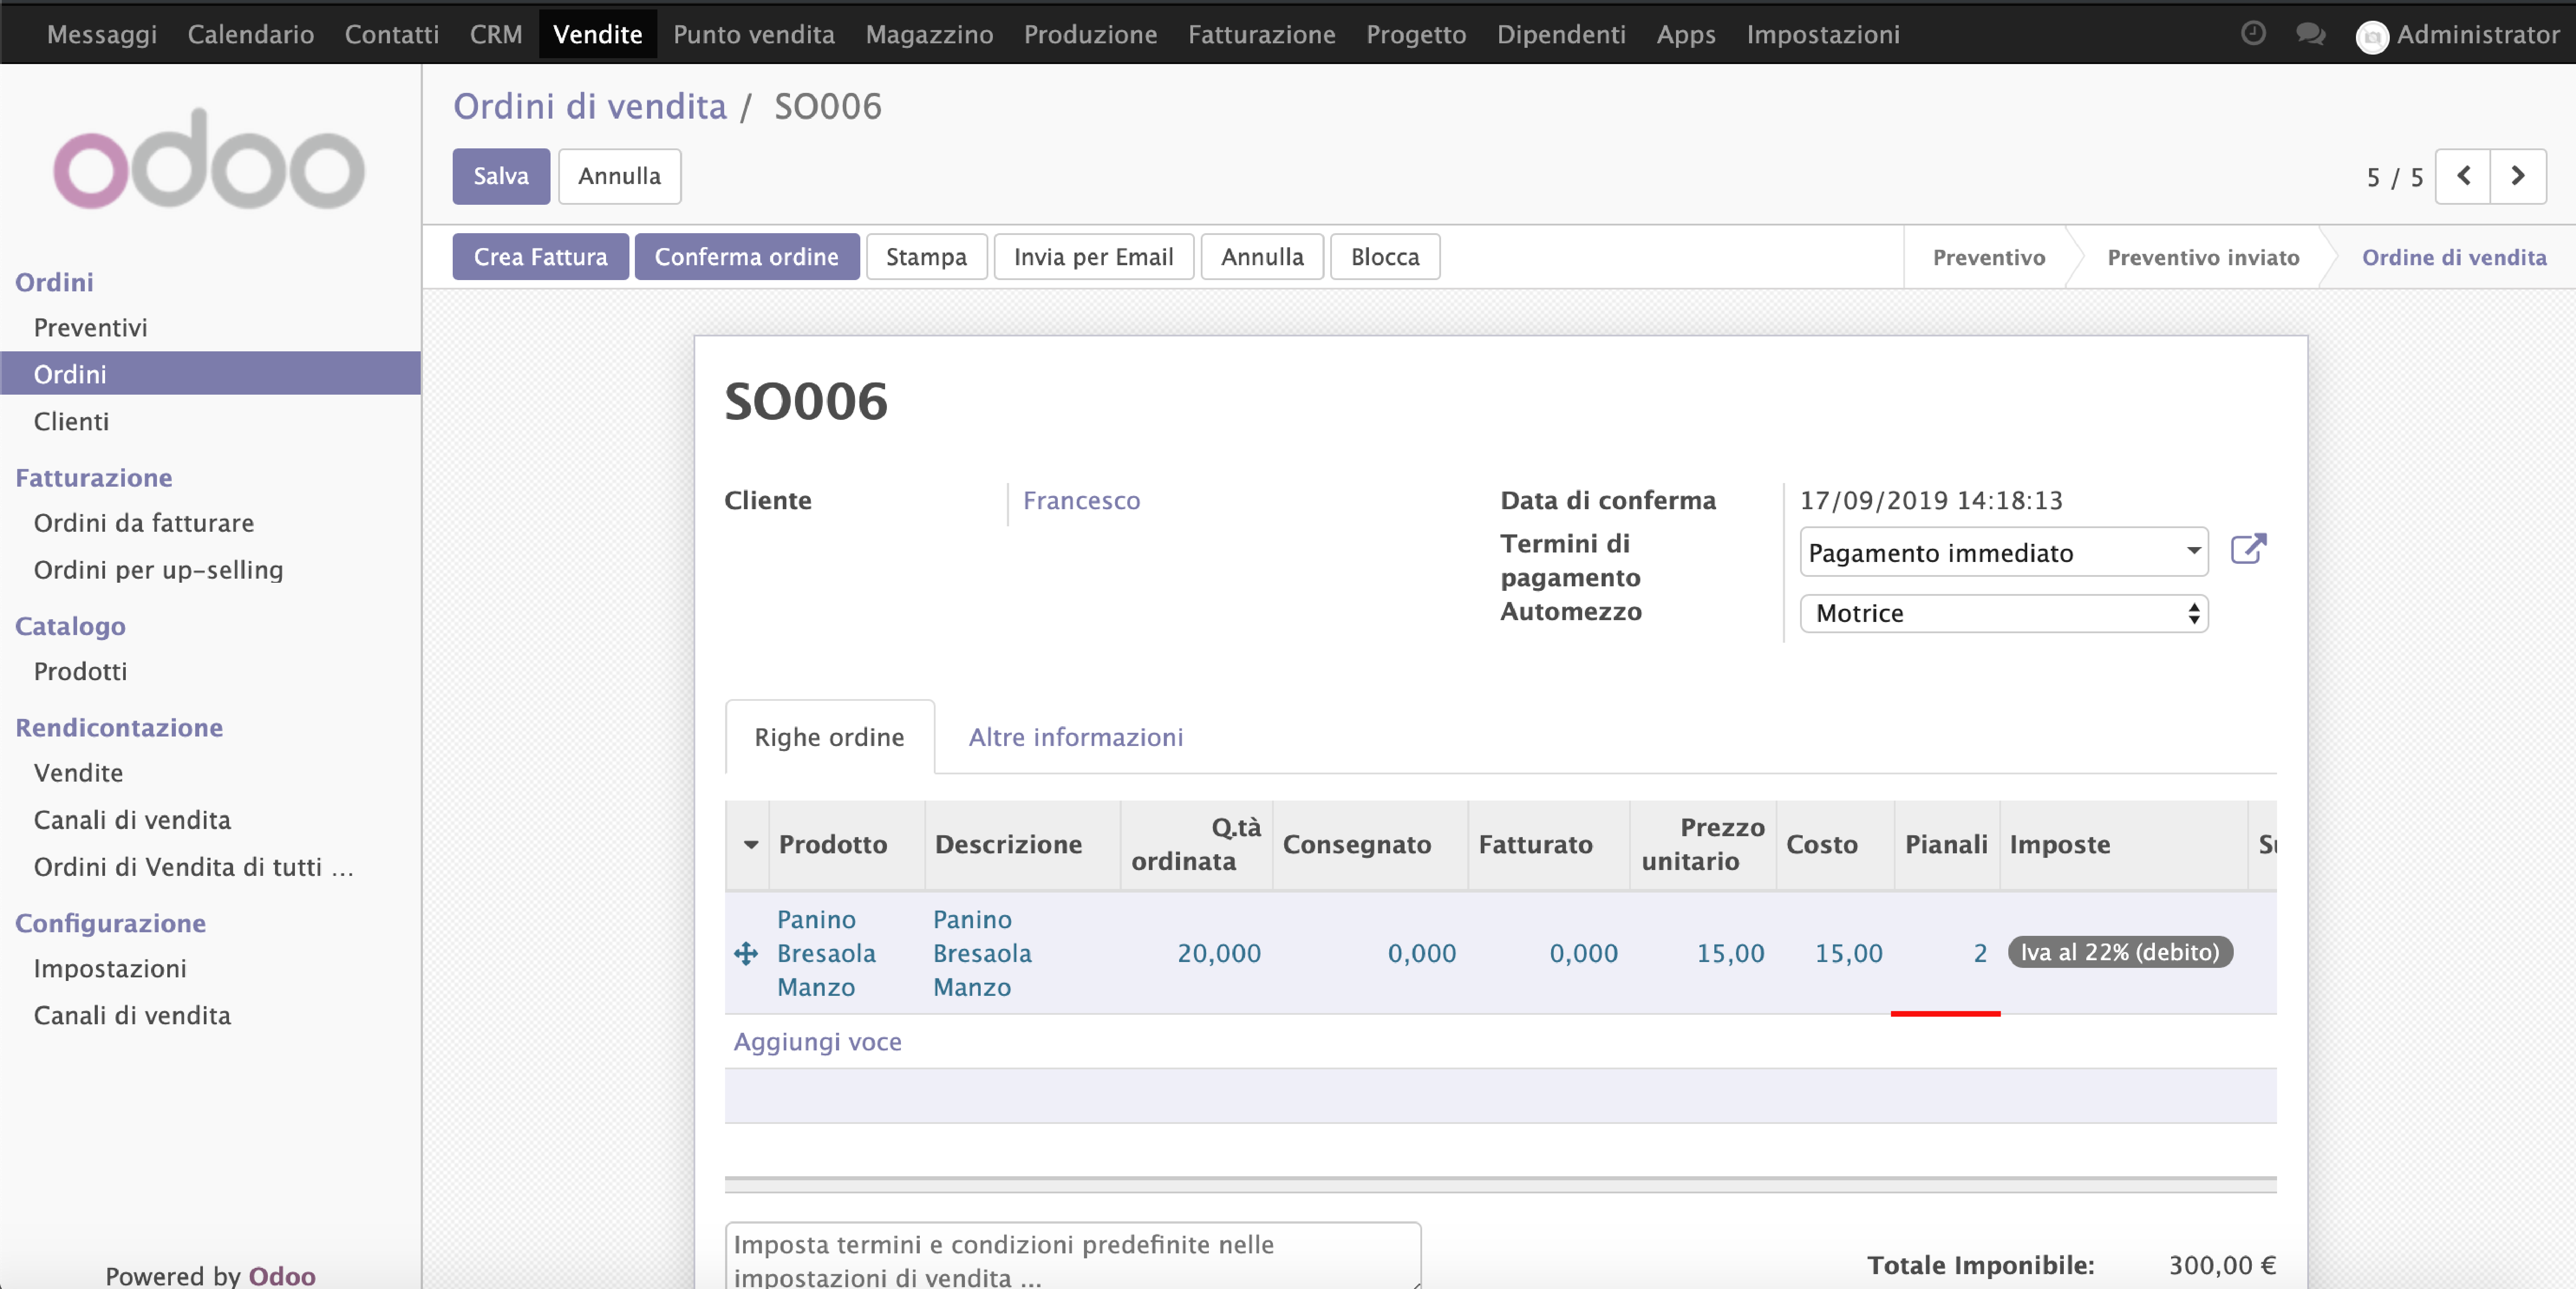
\includegraphics[width=1\linewidth]{figures/test_one}
%	\end{center}
%\end{figure}
%
%\end{frame}
%
%\begin{frame}{Test di sistema e collaudo}
%’Pianali’: \'e dato dal rapporto fra Quantit\'a ordinata (5) / Quantit\'a per confezione (5) = 1.
%
%\begin{figure}[H]
%	\begin{center} 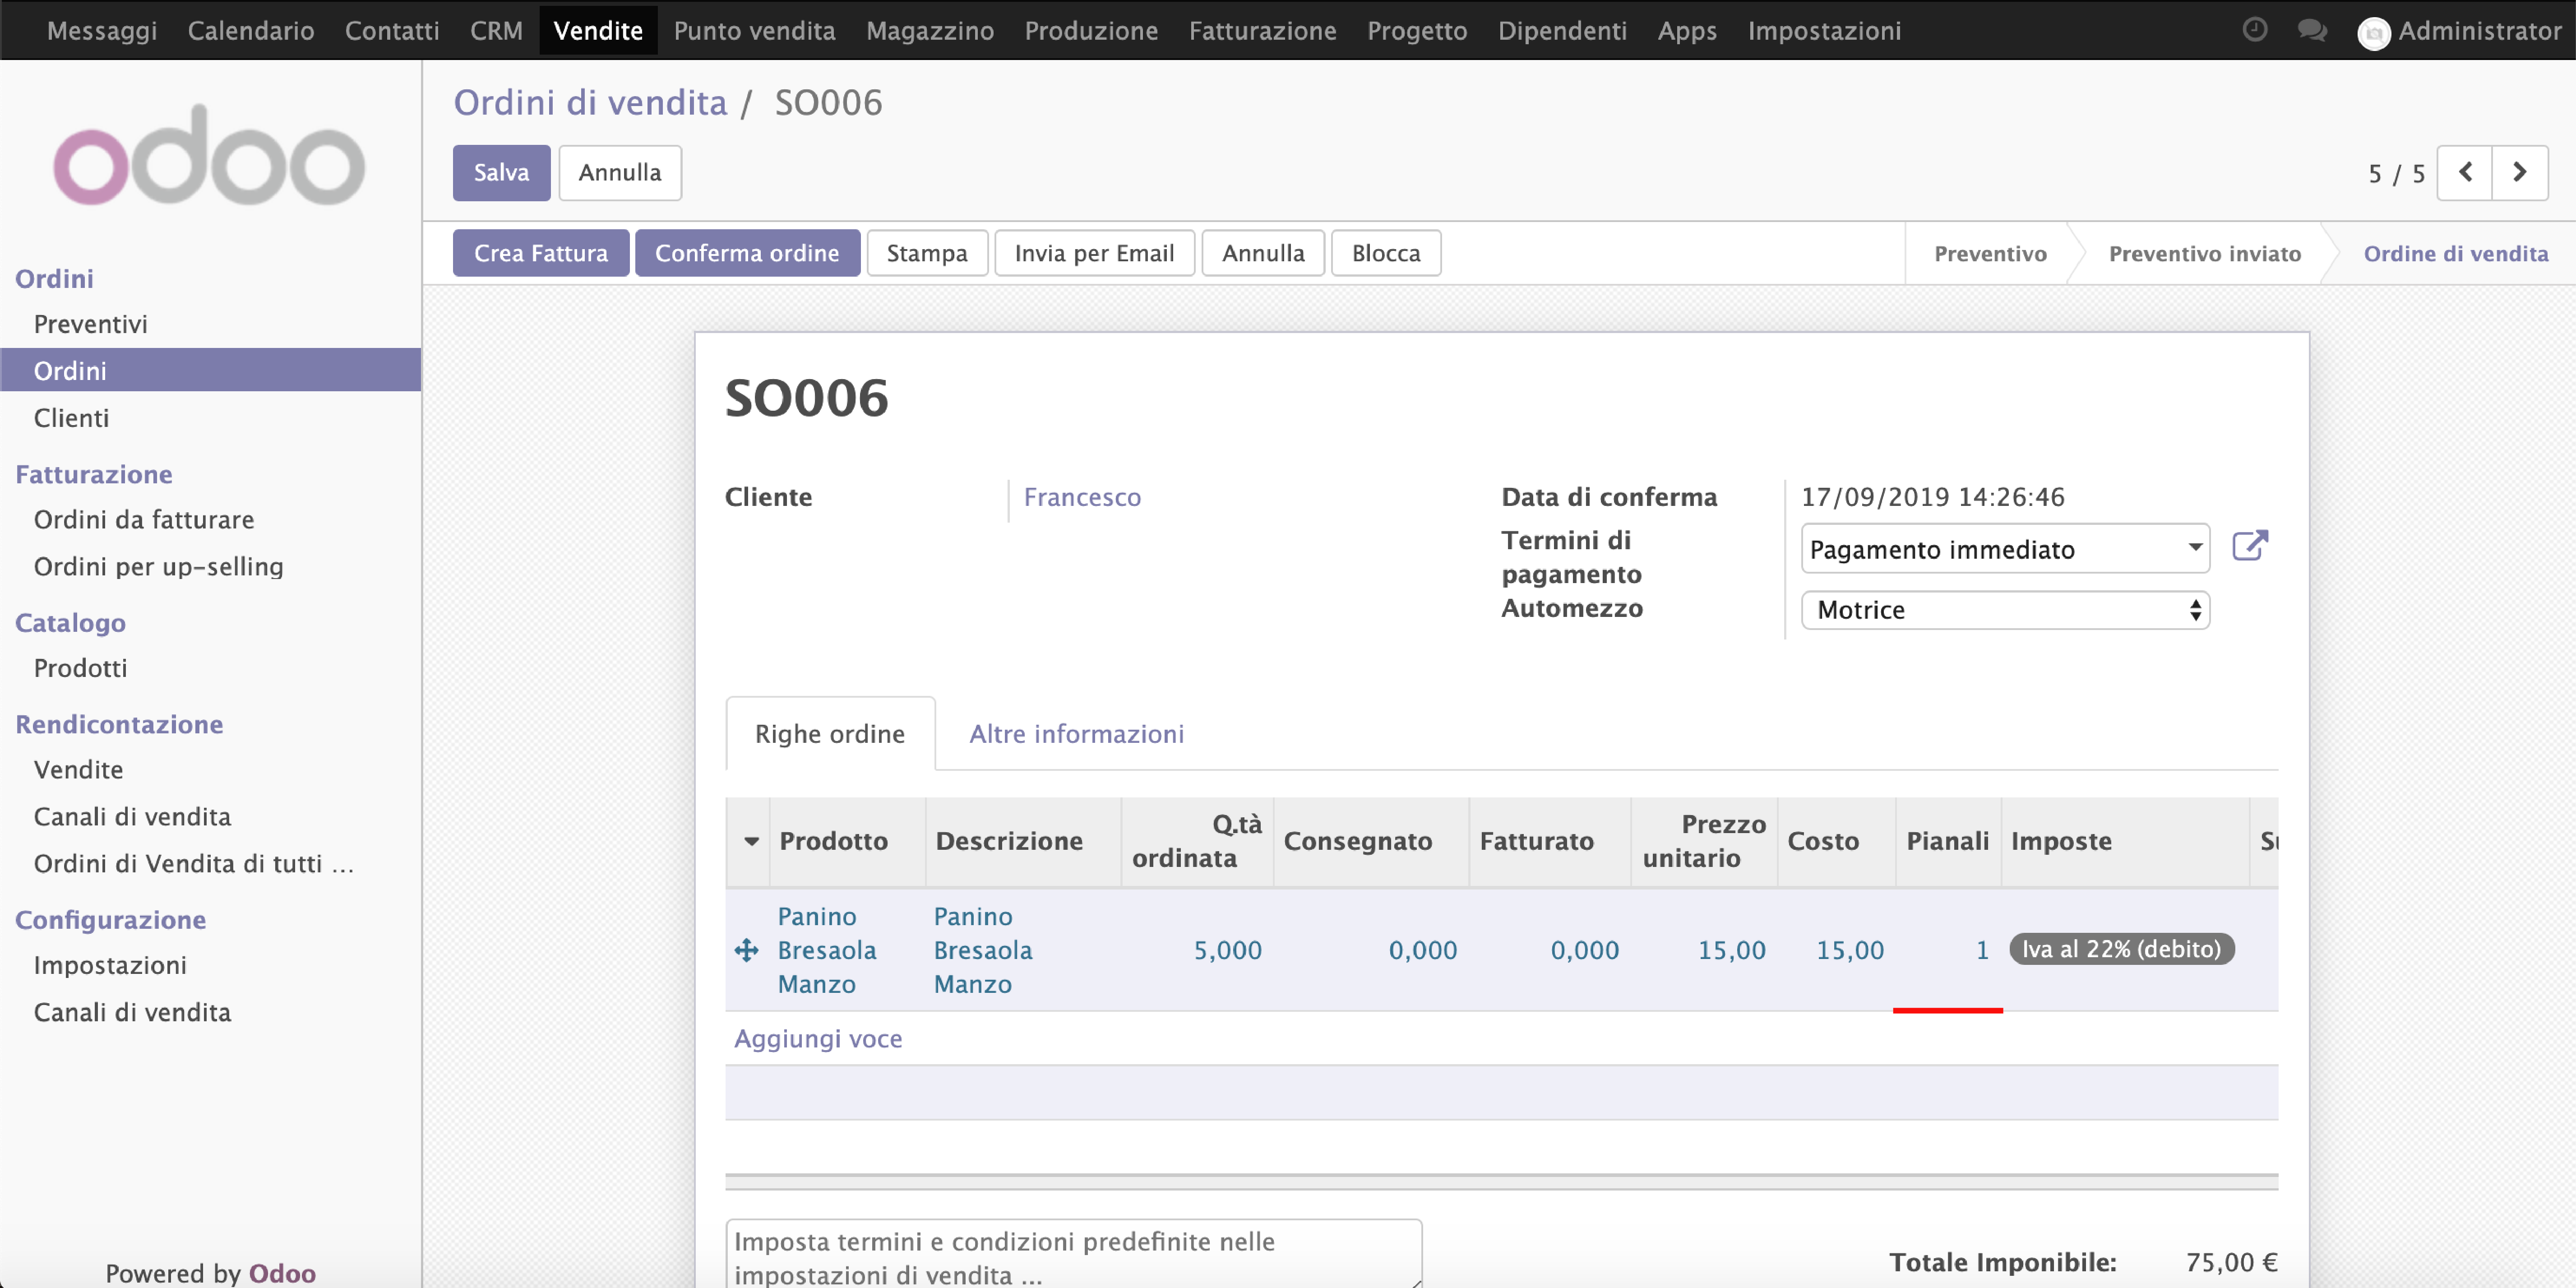
\includegraphics[width=1\linewidth]{figures/two_test}
%	\end{center}
%\end{figure}
%
%\end{frame}
%
%\begin{frame}{Test di sistema e collaudo}
%’Pianali’: \'e dato dal rapporto fra Quantit\'a ordinata (1) / Quantit\'a per confezione (5) = 0,2.
%
%\begin{figure}[H]
%	\begin{center} 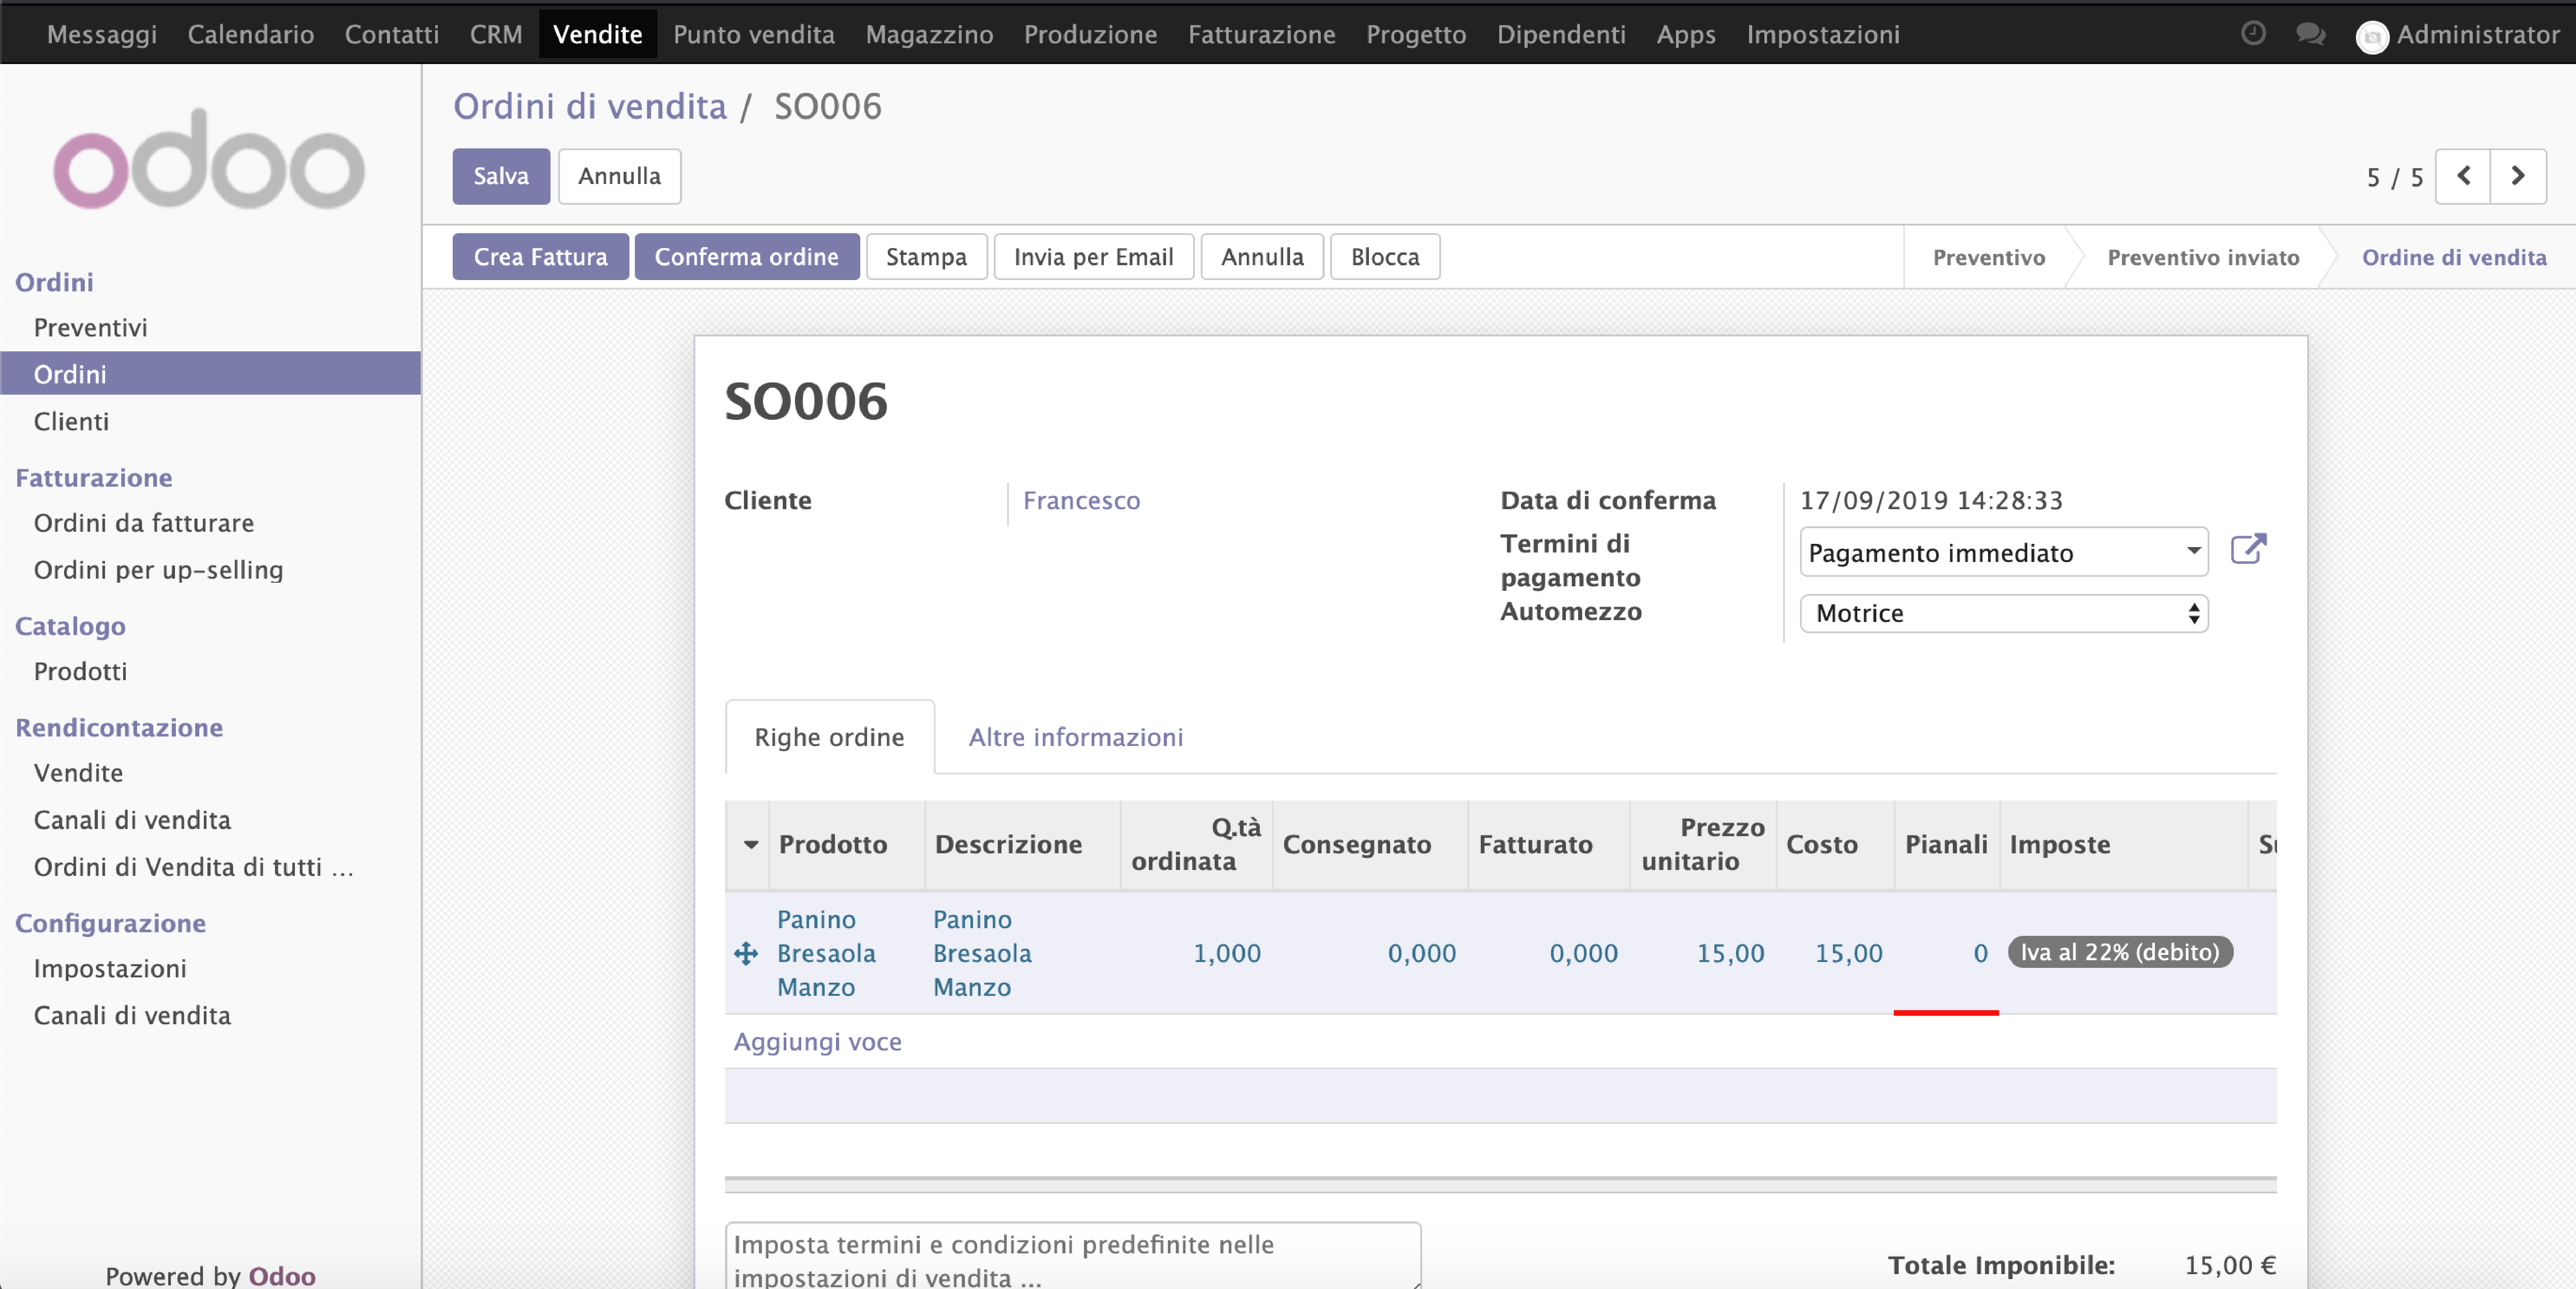
\includegraphics[width=1\linewidth]{figures/three_test}
%	\end{center}
%\end{figure}
%
%\end{frame}

\begin{frame}{Blocco Scaduto\scriptsize{(my\_project)}}
\begin{figure}[H]
	\begin{alertblock}{Obiettivo}
		 Viene raggiunto lo stato Blocco Scaduto quando stiamo confermando un ordine con una data di scadenza antecedente a quella attuale, vuol dire che l’ordine di vendita \'e gi\'a scaduto.
	\end{alertblock}	
\end{figure}

\end{frame}

\begin{frame}{Test di sistema e collaudo}

\begin{figure}[H]
	\begin{center} 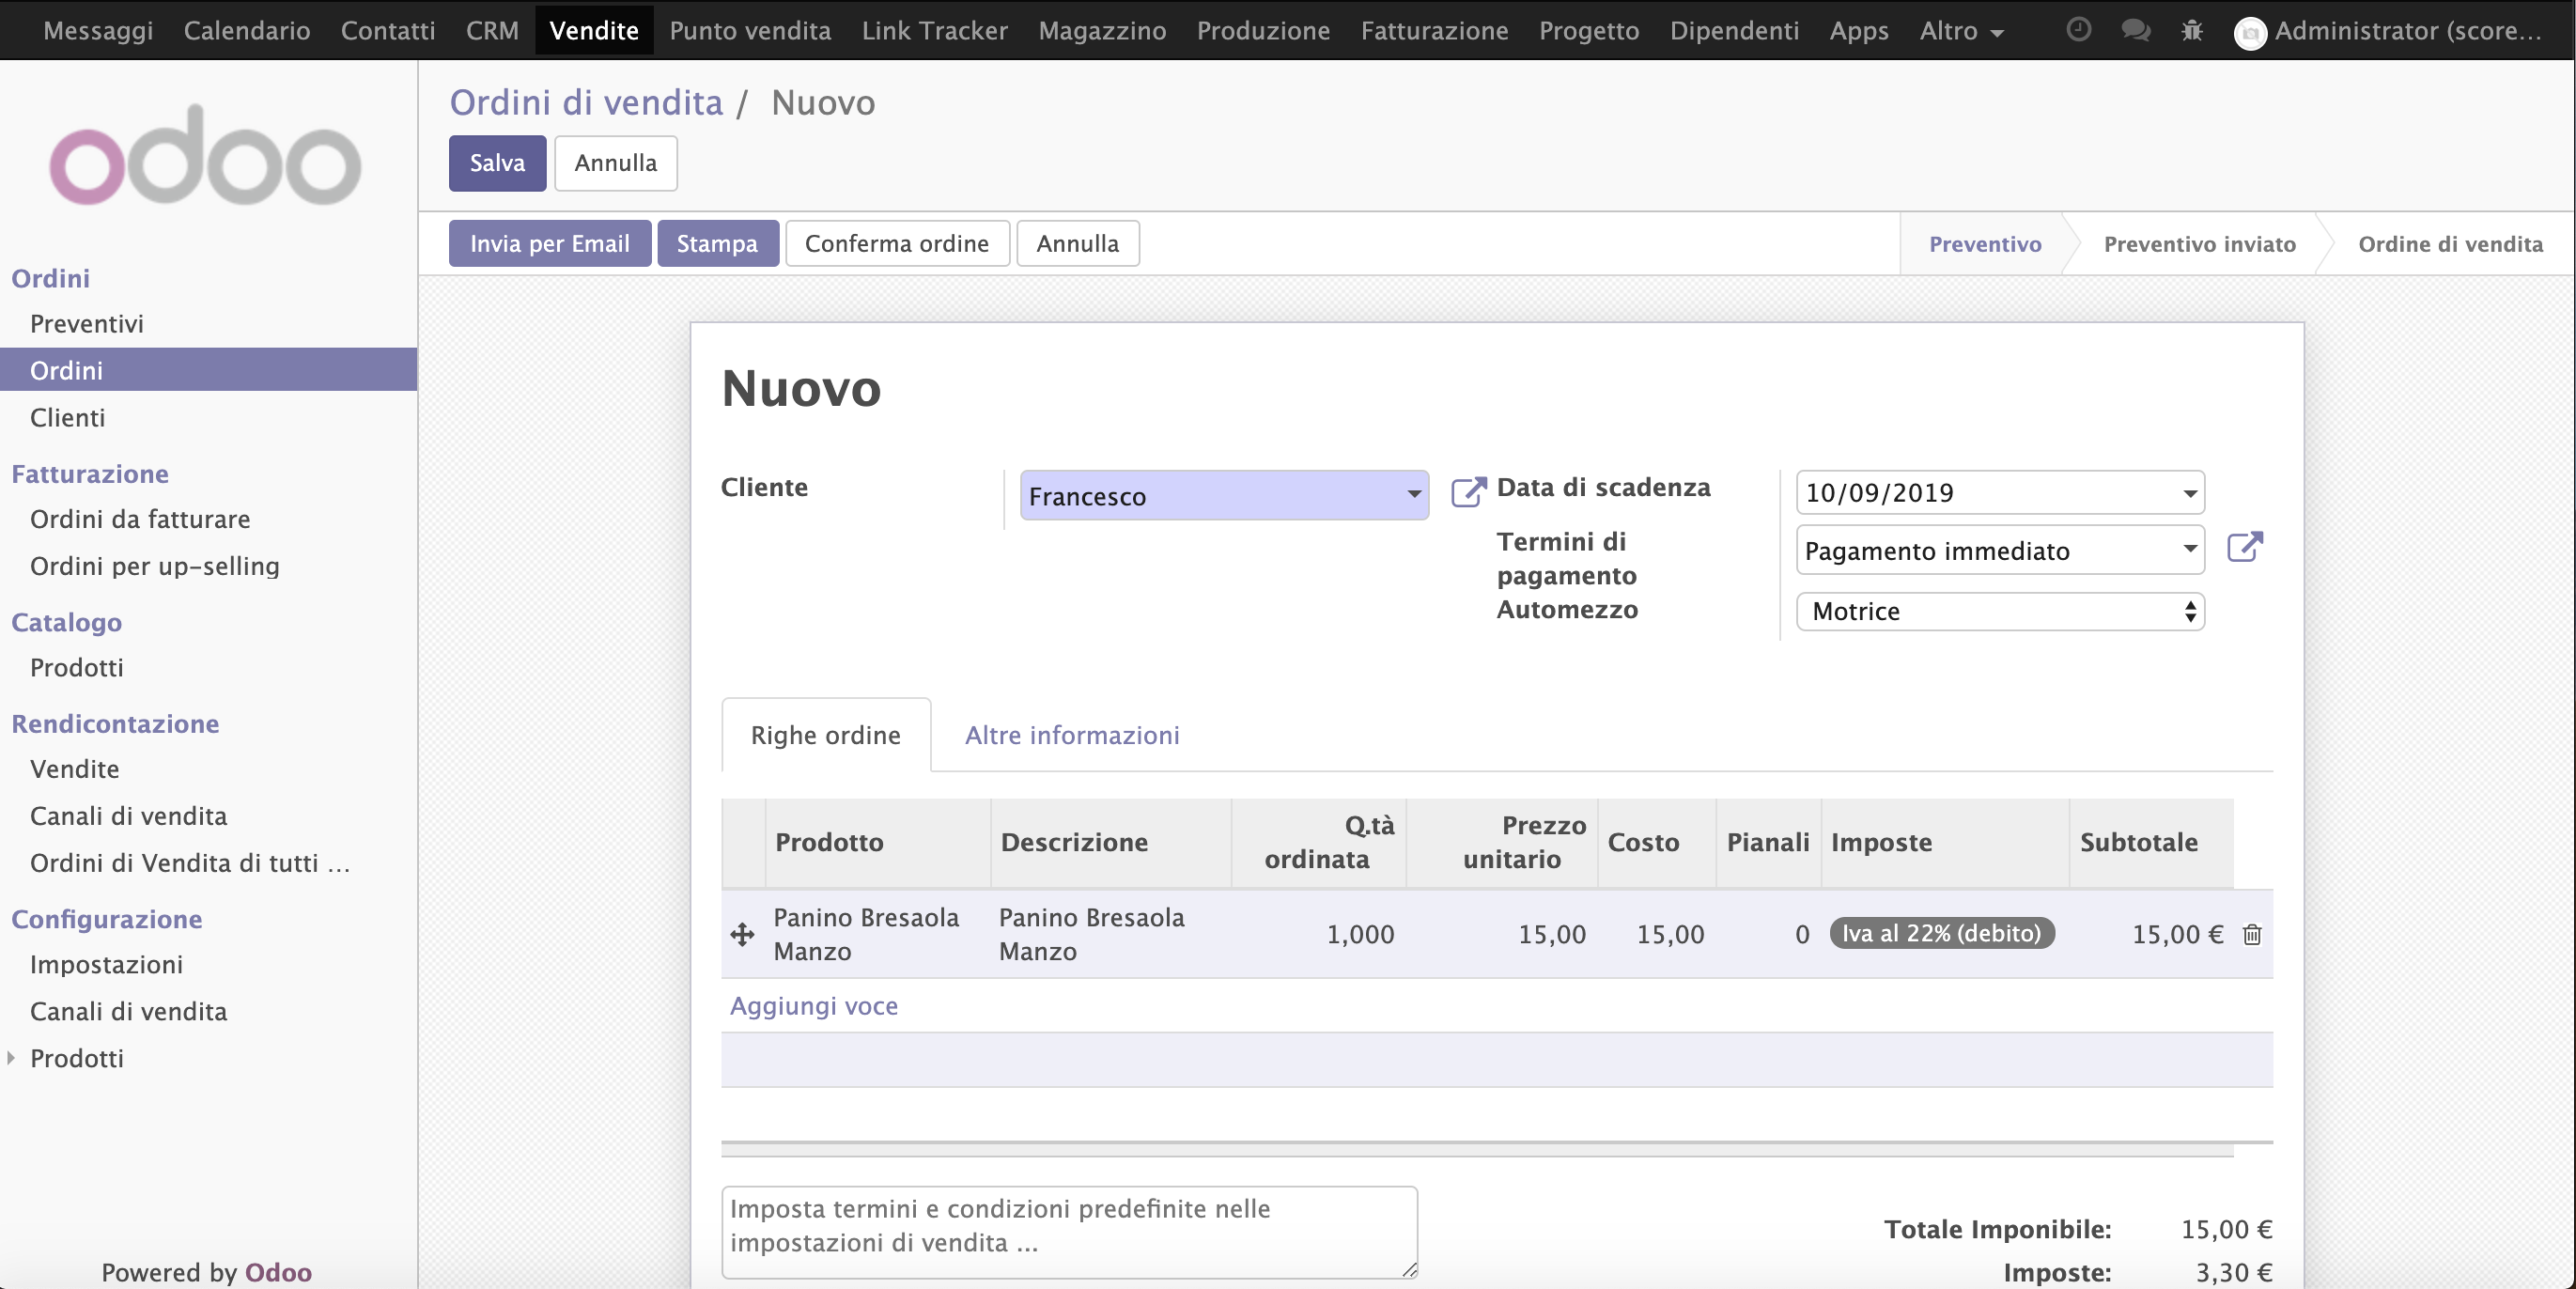
\includegraphics[width=1\linewidth]{figures/exp_one}
	\end{center}
\end{figure}

\end{frame}

\begin{frame}{Test di sistema e collaudo}

\begin{figure}[H]
	\begin{center} 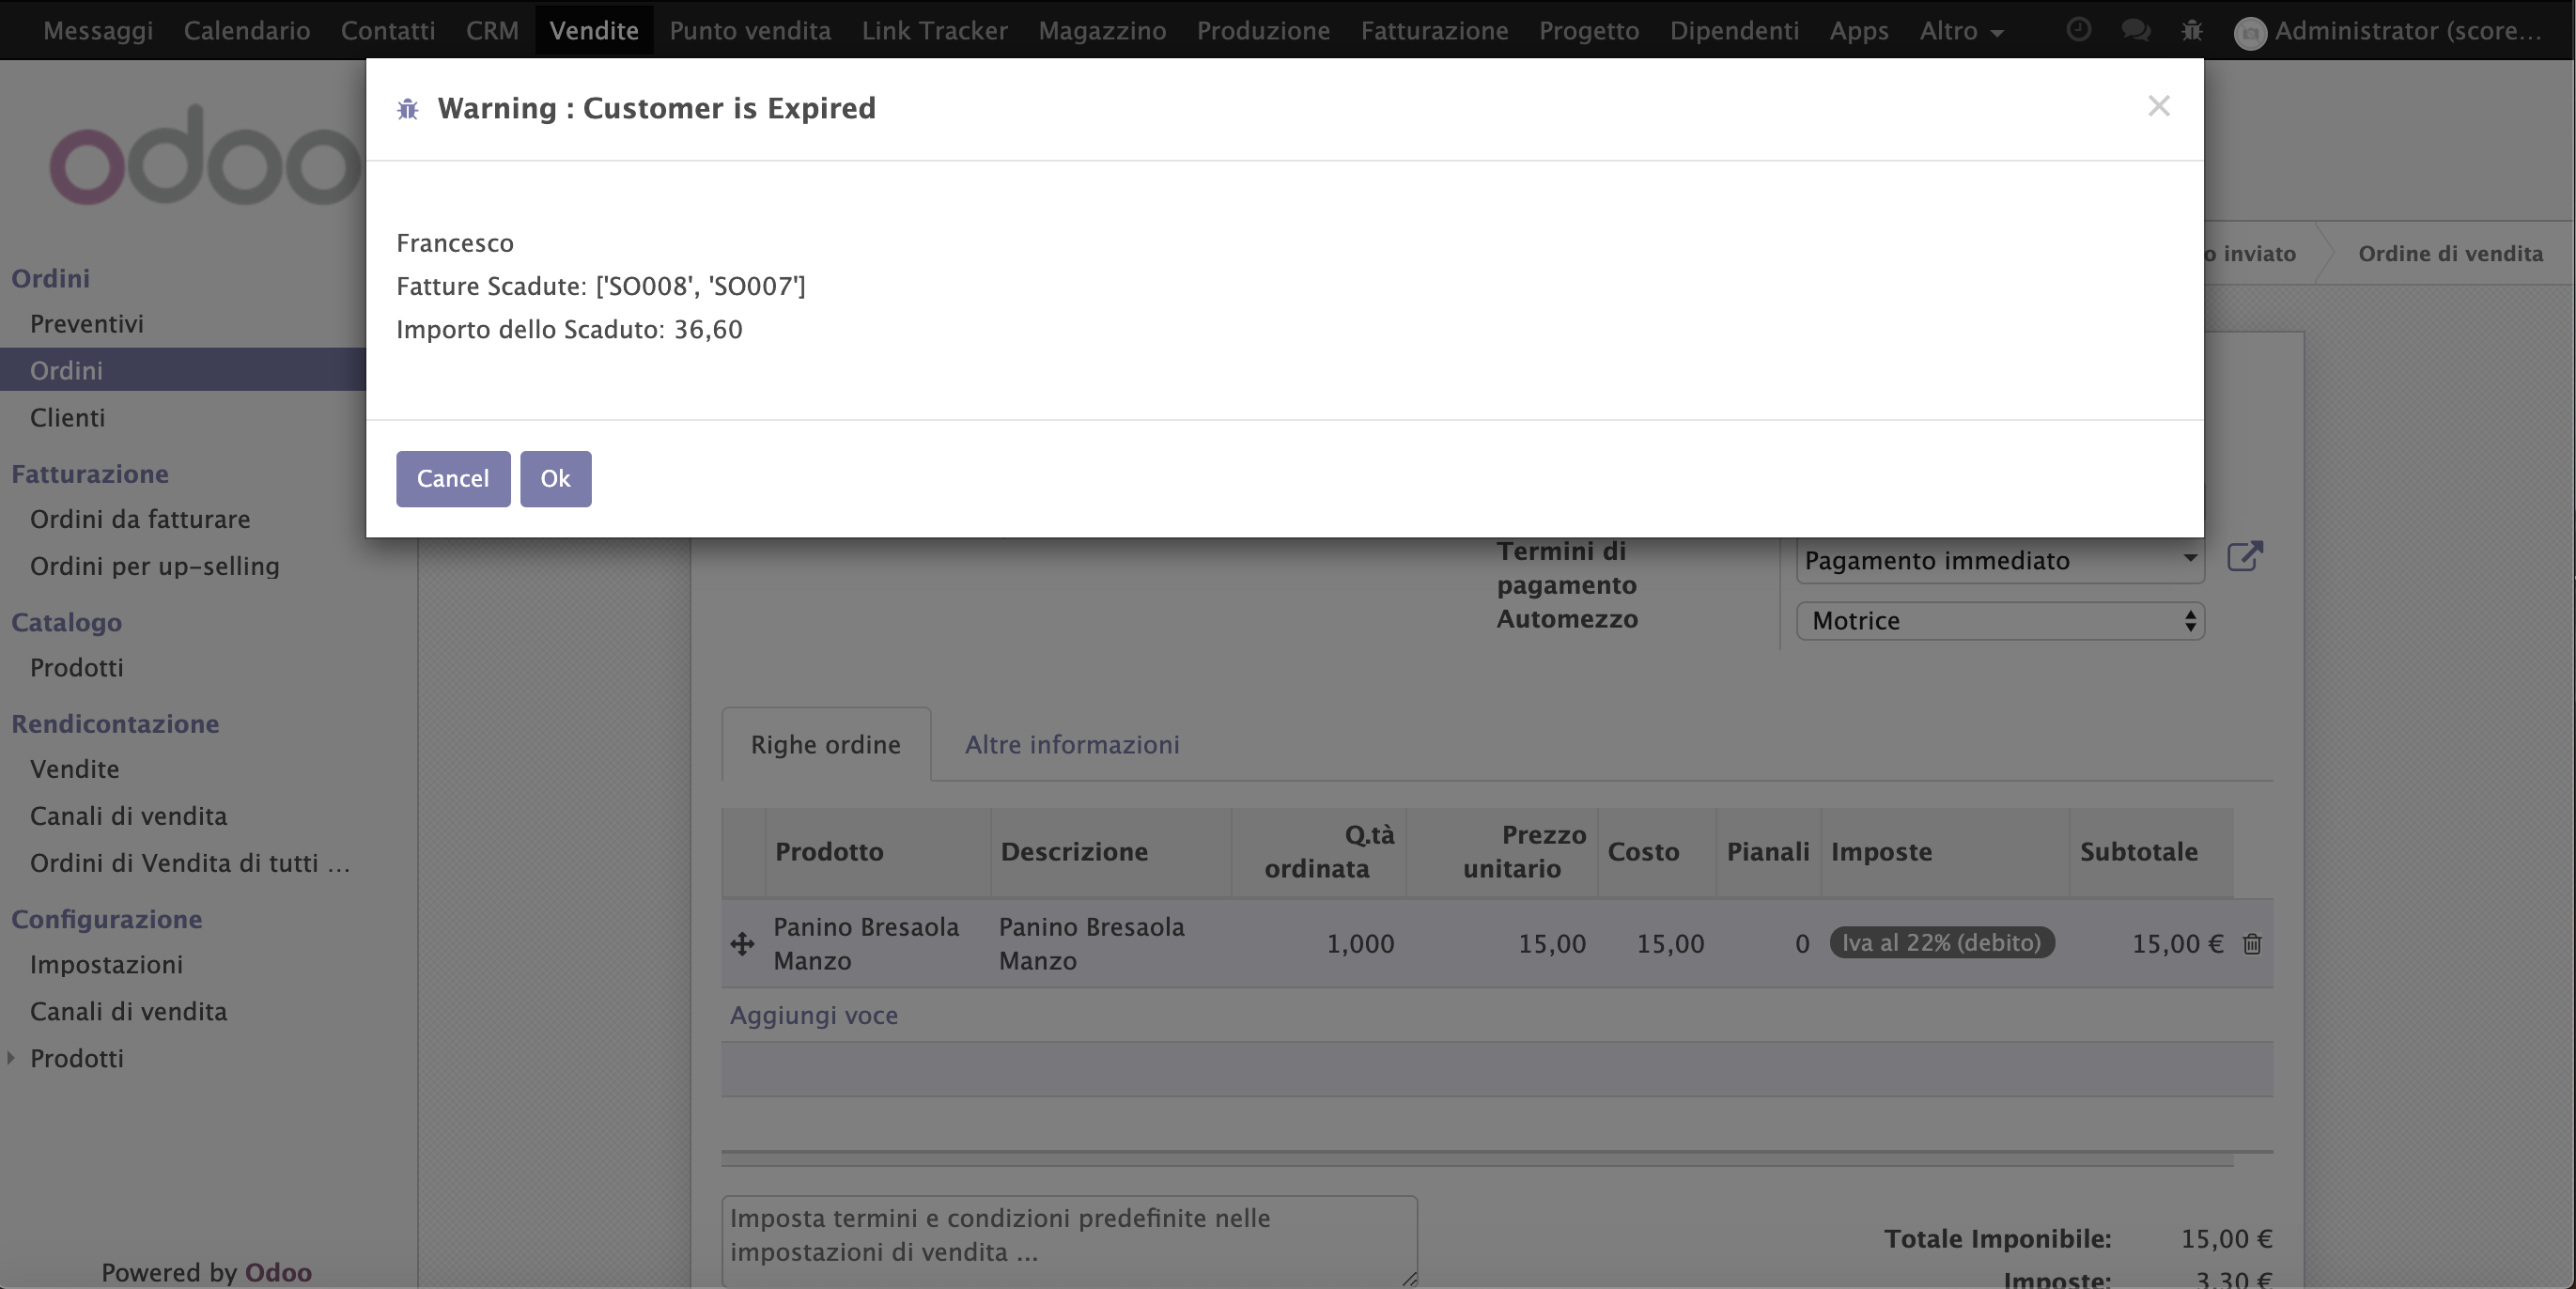
\includegraphics[width=0.95\linewidth]{figures/exp_two}
	\end{center}
\end{figure}

Inoltre verr\'a inviata una mail al direttore commerciale, che sar\'a informato dell'errore al relativo ordine di vendita.
\end{frame}

\begin{frame}{Test di sistema e collaudo}

\begin{figure}[H]
	\begin{center} 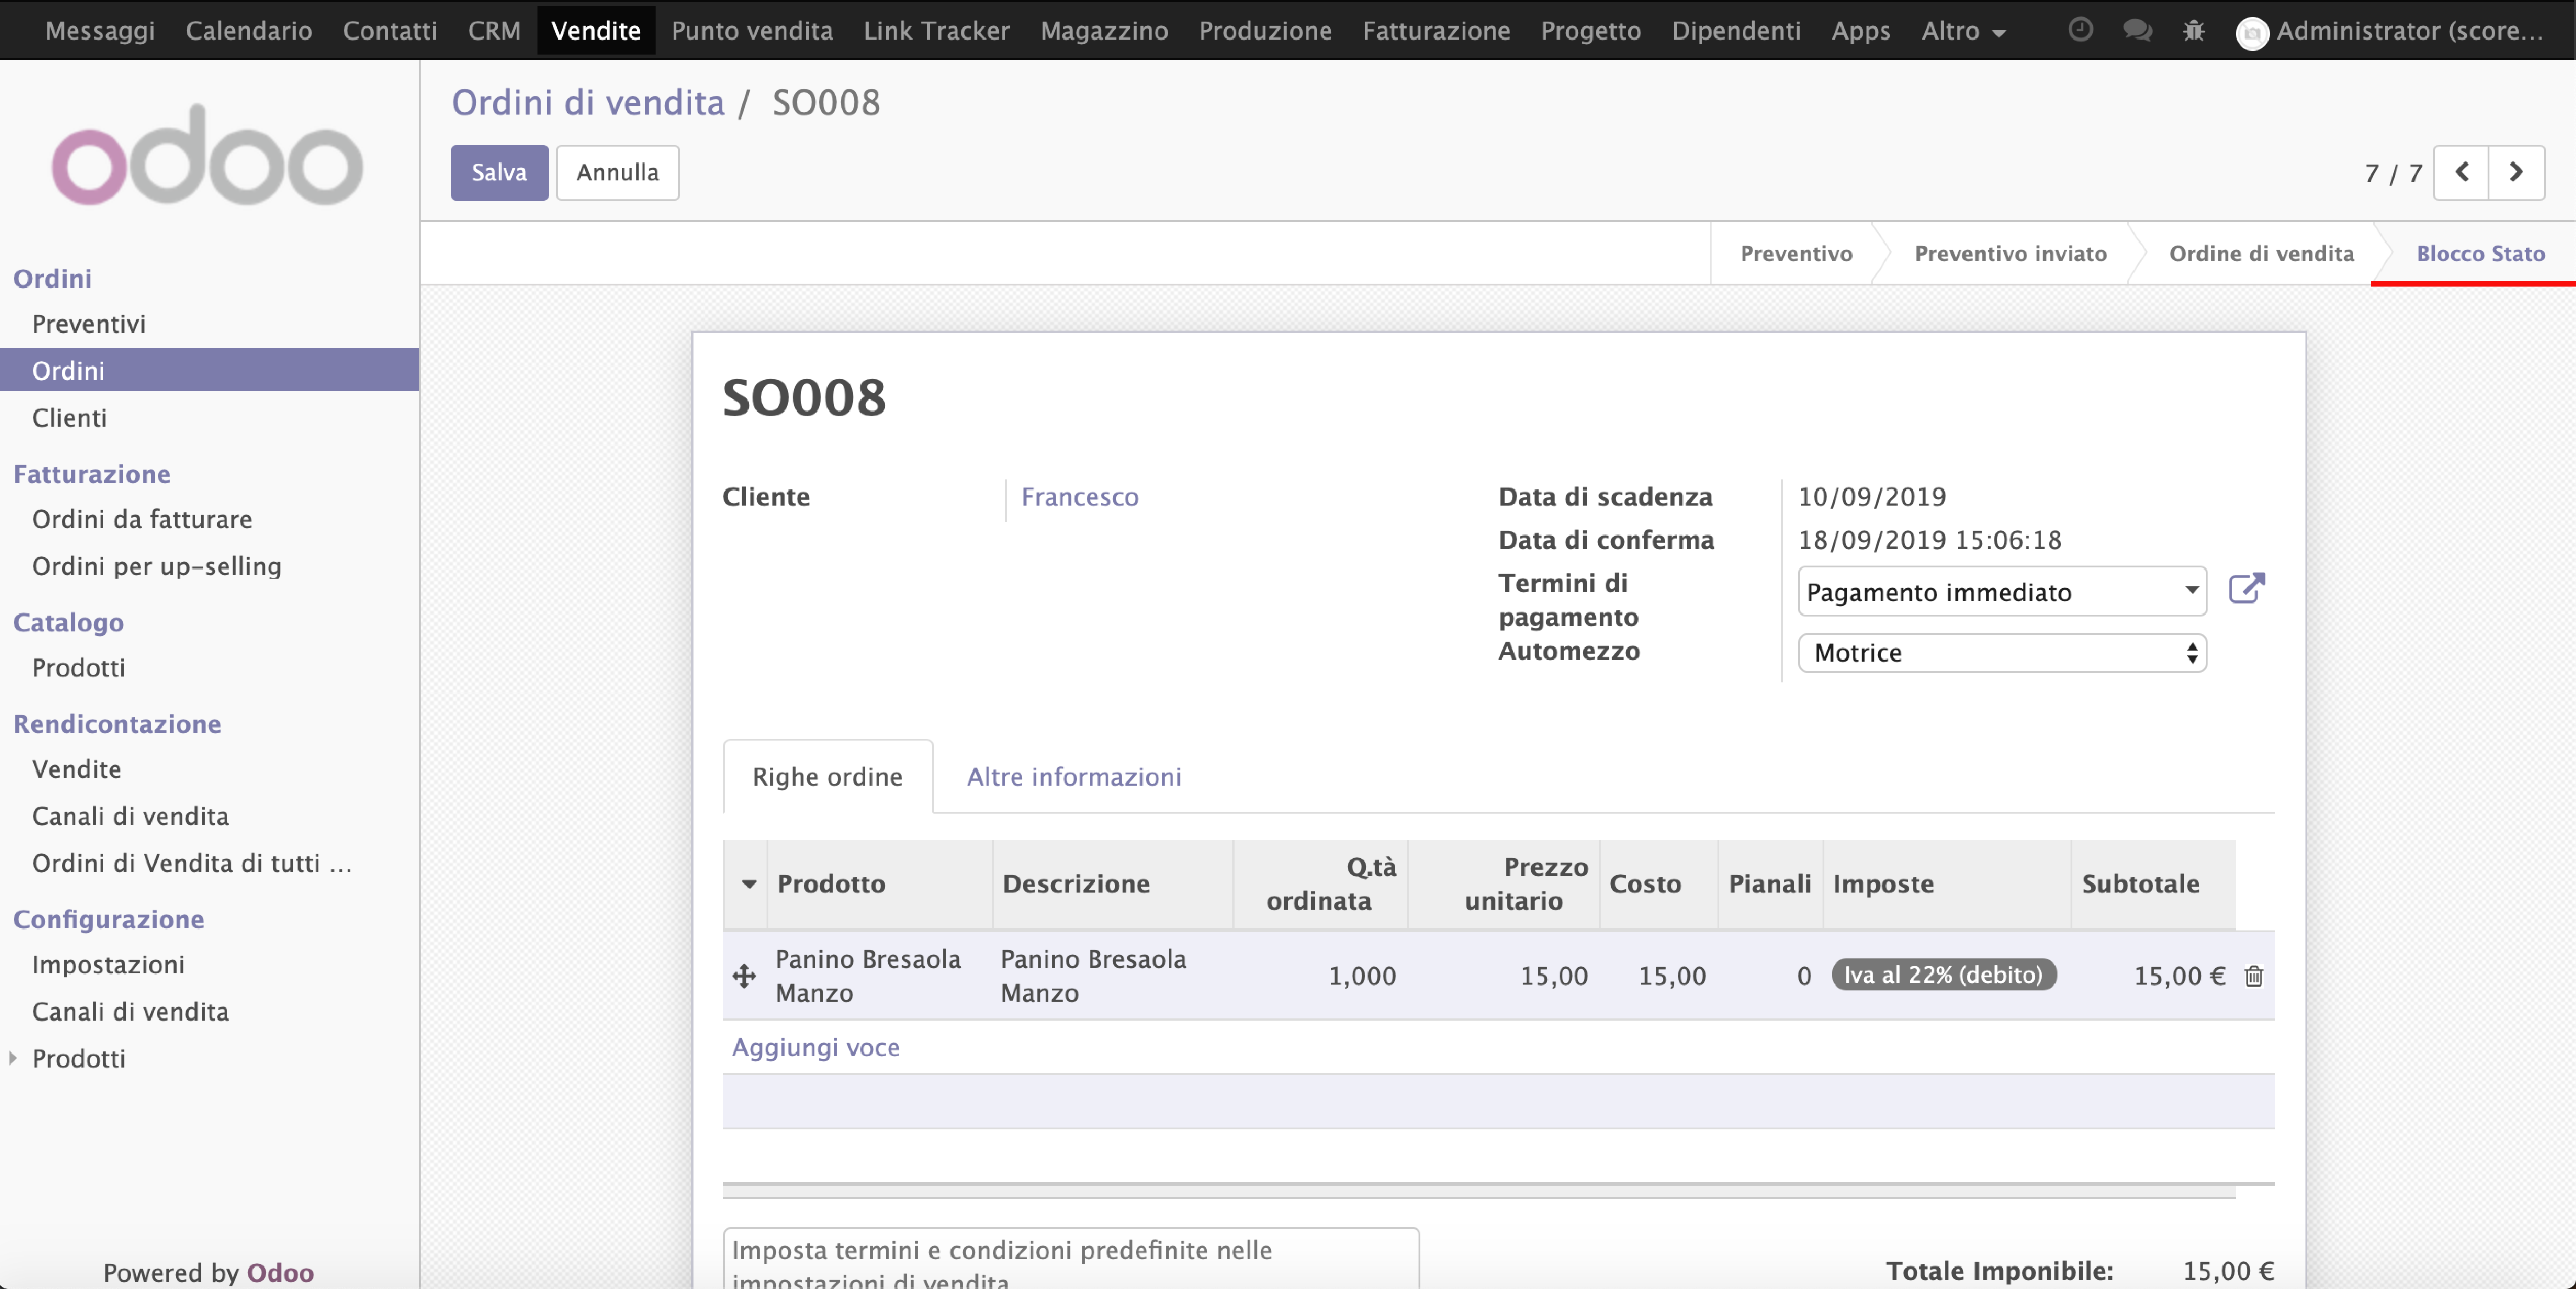
\includegraphics[width=1\linewidth]{figures/exp_three}
	\end{center}
\end{figure}

\end{frame}

\begin{frame}{Test di unità}
Svolti per verificare il codice di ogni modulo.


\begin{figure}[H]
	\begin{center} 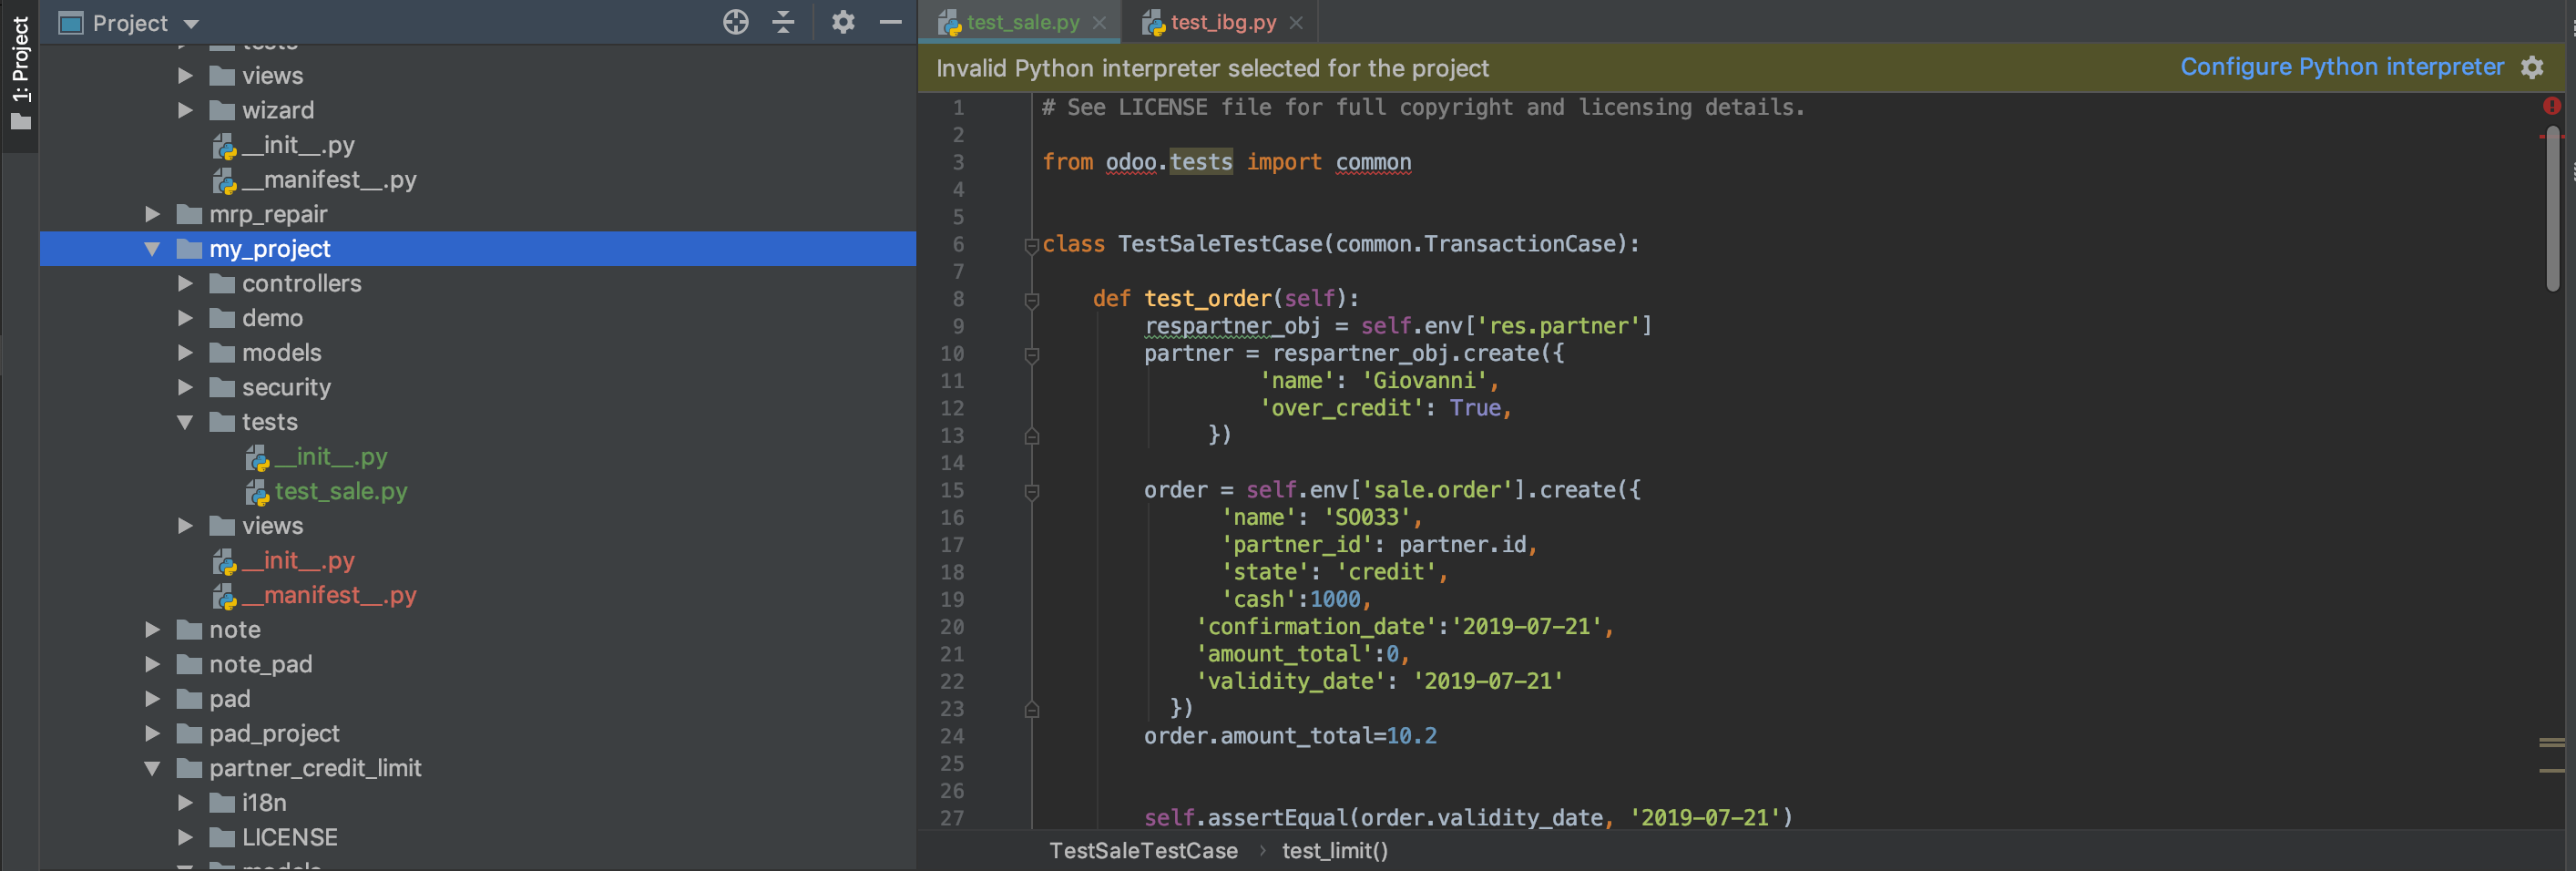
\includegraphics[width=1\linewidth]{figures/unit_test}
	\end{center}
\end{figure}

\end{frame}



\section{Raggiungimento degli obiettivi}
\begin{frame}{Raggiungimento degli obiettivi}
	Lo sviluppo di ciascun modulo prevedeva i seguenti obiettivi:
	\begin{itemize}
		\item Implementazione di un modulo che si occupa di ottimizzare il cosiddetto Time-to-Market
		\item Capacità di raggiungere gli obbiettivi richiesti in autonomia
		seguendo il programma	
		\item Portare a termine le modifiche richieste dal cliente con una percentuale di superamento degli item di collaudo pari al 50\%
	\end{itemize}
	
	Due variazioni nel corso dello stage:
	\begin{itemize}
		\item Test dei moduli eseguiti alla fine dello sviluppo degli stessi
%		\item Cambiamenti in corso d'opera
		\item Realizzazione test di unità non preventivati
	\end{itemize}
\end{frame}



\begin{frame}{Consuntivo}
	In generale il periodo di stage ha richiesto:
	\begin{center}
		\begin{tabular}{|c|l|c|c|}
			\hline
			\textbf{\#} & \textbf{Obiettivi} & \textbf{Ore previste} & \textbf{Ore effettive} \\\hline
			1           & Formazione               & 208                   & 180                   \\\hline
			2           & Sviluppo moduli            & 72                    & 100                     \\\hline
			3           & Collaudo finale      & 40                     & 40                     \\\hline
		\end{tabular}
	\end{center}
	Cause cambiamenti tempistiche:
	\begin{itemize}
		\item Formazione pi\`u breve
		\item Sviluppo moduli più approfondita, causa mancate funzionalità affrontate
		\item Testing e collaudo rispettati
	\end{itemize}
\end{frame}
\section{Conclusioni}
\begin{frame}{Conclusioni}
Sviluppi futuri:
\begin{itemize}

\item Nuovo pannello di ricerca dove sarà possibile utilizzare un checkbox come filtro;
\item Miglioramento del funzionamento dell'inventario: inserimento nuovi campi nella vista "Ordini di consegna" del modulo magazzino.
\end{itemize}
	\vspace{0.5cm}
	\begin{enumerate}
		\item Tutti gli obiettivi sono stati raggiunti
		\item Realizzazione test aggiuntivi
		\item Valutazione positiva dei risultati forniti
		\item Importanti conoscenze apprese
	\end{enumerate}
				

	
\end{frame}

%
%{
%\definecolor{mycolor}{HTML}{B71C1C}
%\begin{frame}
%\pagecolor{mycolor}
%\end{frame}
%}

\end{document}
